%\documentstyle[11pt,twoside,psfig]{report}
\documentclass[11pt,twoside]{report}
\usepackage{graphicx}
\usepackage{makeidx}
%\usepackage{showidx}  % Shows index entries at edge of page
\pagestyle{headings}

%-----------------------------------------------------------------------
\topmargin 0.1in
\oddsidemargin 0.1in
\evensidemargin 0.1in
\textheight 8.5in
\textwidth 6.25in
\headheight 0.20in
\headsep 0.3in
\parindent 0in
\parskip \bigskipamount

\newcounter{bean}
\newenvironment{romanlist}%
{\begin{list}%
{(\roman{bean})}{\topsep 0in \usecounter{bean}}}%
{\end{list}}

\newcommand{\AU}{{\rm AU}}
\newcommand{\cs}{c_{S}}
\newcommand{\degree}{{\nobreak^{\circ}}}
\newcommand{\e}[1]{\mbox{$\times 10^{#1}$}}
\newcommand{\eg}{{\it e.g.\,}}
\newcommand{\ea}{{\it et al.\,}}
\newcommand{\EpsL}{\varepsilon_{L}}
\newcommand{\etc}{{\it etc.\,}}
\newcommand{\ghz}{{\rm\,GHz}}
\newcommand{\Halpha}{\mbox{${\rm H\alpha}$}}
\newcommand{\HCO}{{\rm HCO^{+}}}
\newcommand{\HI}{{\rm H^{0}}}
\newcommand{\HII}{{\rm H^{+}}}
\newcommand{\Hz}{{\rm\,Hz}}
\newcommand{\TwoH}{{\rm H_{2}}}
\newcommand{\ie}{{\it i.e.\,}}
\newcommand{\Junits}{{\rm cm^{2}s^{-1}}}
\newcommand{\SIJunits}{{\rm m^{2}s^{-1}}}
\newcommand{\K}{{\rm\,K}}
\newcommand{\khz}{{\rm\,KHz}}
\newcommand{\km}{{\rm\,km\,}}
\newcommand{\kms}{{\rm\,km\,s^{-1}}}
\newcommand{\Lstar}{L_{*}}
\newcommand{\Lsun}{L_{\odot}}
\newcommand{\Mdot}{\dot{M}}
\newcommand{\m}{{\rm\,m}}
\newcommand{\mm}{{\rm\,mm}}
\newcommand{\mhz}{{\rm\,MHz}}
\newcommand{\micron}{{\rm $\,\mu m$}}
\newcommand{\Msun}{M_{\odot}}
\newcommand{\MuL}{\mu_{L}}
\newcommand{\NI}{{\rm [N^{0}]}}
\newcommand{\NII}{{\rm [N^{+}]}}
\newcommand{\OI}{{\rm [O^{0}]}}
\newcommand{\OII}{{\rm [O^{+}]}}
\newcommand{\parsec}{{\rm\,pc}}
\newcommand{\perm}{{\rm\,m^{-3}}}
\newcommand{\percm}{{\rm\,cm^{-3}}}
\newcommand{\perparsec}{{\rm\,pc^{-1}}}
\newcommand{\peryr}{{\rm\,yr^{-1}}}
\newcommand{\Piv}{\Pi_{v}}
\newcommand{\ro}{\mbox{$r_{0}$}}
\newcommand{\rA}{\mbox{$r_{A}$}}
\newcommand{\Rsun}{R_{\odot}}
\newcommand{\SI}{{\rm [S^{0}]}}
\newcommand{\SII}{{\rm [S^{+}]}}
\newcommand{\simlt}{\stackrel{<}{_{\sim}}}
\newcommand{\simgt}{\stackrel{>}{_{\sim}}}
\newcommand{\Tdyn}{T_{dyn}}
\newcommand{\thz}{{\rm\,THz}}
\newcommand{\water}{\mbox{$\rm H_{2}O$}}

\newcommand{\ApJ}{{\it Ap.J.}, }
\newcommand{\ApJLett}{{\it Ap.J.Letters.}, }
\newcommand{\MN}{{\it M.N.R.a.S.}, }
\newcommand{\AJ}{{\it A.J.}, }
\newcommand{\AAp}{{\it A \& Ap.}, }
\newcommand{\vol}[1]{{\bf #1}}

\setcounter{secnumdepth}{3}
\setcounter{tocdepth}{2}
\pagenumbering{roman}
\makeindex
%-----------------------------------------------------------------------

\begin{document}

% \vspace*{-1in}
\title{SPECX V6.3\\
         Users' Manual}
\author{Rachael Padman\\
        Cavendish Laboratory\\
        Madingley Rd\\
        Cambridge\\
        CB3 OHE\\
        ENGLAND\\
        \\
        (RACHAEL @ MRAO.CAM.AC.UK\\
        \& RP1 @ STAR.AST.CAM.AC.UK)}
\date{18th September 1993}

\maketitle
\cleardoublepage
\tableofcontents

\cleardoublepage
\part{Users' Guide}
\chapter{Introduction}
\pagenumbering{arabic}

SPECX is a general purpose program, originally written on the NORD
10/50 of the Mullard Radio Astronomy Observatory, and substantially
updated on the VAX 11/780 of the Department of Astronomy at the
University of California, Berkeley. In 1995 it was ported to UNIX.  It
operates on spectral-line data stored in random access binary
files\index{data files} of arbitrary length. The format of these files
is described in detail in Appendix F. SPECX is sufficiently flexible
that data from most instruments can be handled by the program, and has
been used to reduce data from the mm and sub-mm spectral-line
receivers at UKIRT\index{UKIRT} and JCMT\index{JCMT}, from the 14-m
dish of the FCRAO\index{FCRAO}, from Onsala\index{Onsala} and from the
11-metre and 300-foot telescopes of the NRAO\index{NRAO}.

SPECX makes use of either the MONGO\index{MONGO} graphics package
FORTRAN subroutine library, or of the PGPLOT\index{PGPLOT}
library. These packages includes interactive
graphics\index{graphics!interactive!see: interactive graphics}
\index{interactive graphics} via the cursor\index{graphics cursor} on
VT100/Retrographics and other Tektronix-emulation
terminals\index{terminals}, and in the case of PGPLOT graphics, with
X-terminals also. If the terminal type will permit, as much reduction
as possible is performed in interactive graphics mode.

One of the main reasons for writing the program originally was to
reduce data from the autocorrelation\index{correlator} spectrometer at
UKIRT, and more recently from the DAS at JCMT. Facilities are included
for processing up to eight ``parallel" spectra
(``sectors"\index{sectors}, ``quadrants"\index{quadrants} or
``sub-bands"\index{sub-bands}), which may have the same or different
centre frequencies, resolutions, etc. This feature allows it to
process the eight correlator\index{correlator} channels, different
filter-banks\index{filter-banks}, dual polarization \index{dual
polarization} data, \etc

SPECX is user-friendly\footnote{Some users have disputed this
description, preferring instead the description ``user tolerant''. One
has even described it as ``unpleasant to use and primitive in its
capabilities''. Not so of course, but I am always open to suggestions
that will push the program further in the ``friendly'' direction}. All
input required by the program is prompted for if not specified in the
command line, so that it is not necessary to remember hundreds of
arcane keywords. The individual commands are given informative names,
so that the appropriate command can nearly always be found quickly by
intelligent use of the HELP or SHOW-COMMANDS commands. The command
line interpreter recognizes acceptable abbreviations for all commands,
accepts parameters in free-format, and will accept a number of
commands on one line. The SPECX command language is described in
detail in Chapter 3 of this document. It is not necessary to know more
than the bare minimum about the command language in order to use SPECX
fruitfully, but in fact it is not particularly complicated.

A facility is included for writing the current reduction
environment\index{environment} to a dump (.DMP) file. This may be set
to dump automatically, after each SPECX command or macro, or only when
specifically requested. This facility allows you to recover from a
crash, or return after a coffee-break\index{coffee-break} or whatever
and find all flags, variables and spectra in the same state as when
you left. It is also possible to tailor different incarnations of the
program for different purposes, such as reducing FCRAO data with one
and JCMT data with another.

Several different classes of facility are available in SPECX. These include:
\index{facilities}
\begin{itemize}
\item File handling, and transferring scans to and from data files.
\item Single and multiple scan arithmetic, scan averaging etc.
\item Commands to store partially reduced spectra in storage registers and to
      retrieve spectra from them.
\item Commands for the listing and display of spectra (on e.g.\ a X-device,
      vt-terminal, or Tektronix device).
\item Fitting and removal of polynomial, harmonic and gaussian baselines.
\item Commands for filtering and editing spectra.
\item Commands to determine important line parameters (peak intensity, width,
      etc) .
\item Fourier transform and power spectrum calculation.
\item Assembling a number of reduced individual spectra into a map file,
      and contouring or greyscaling any plane or planes of the resulting cube.
\item The ability to write indirect command files.
\end{itemize}

Please note that SPECX is primarily a tool for manipulating {\em single}
spectra. It is anticipated that once a map\index{map file} file has been
produced that another program will be used to reduce this map (although SPECX
has an excellent set of tools for {\em display}\index{map display} of the map
data). As a result, SPECX does not include facilities for performing reduction
operations on the map, although any individual spectrum can be retrieved,
manipulated and replaced in the map. The plane of the map being contoured is
held in a temporary storage file
\texttt{mapplane.tmp}\index{mapplane.tmp@\verb+mapplane.tmp+}, and the last version is
not deleted after use. This is a simple binary file, with record length equal
to the number of points in a row, which can be read or mapped to an array in
another program or read directly by the IMAGE
\index{Image (MONGO command)} command in Berkeley/MRAO MONGO\index{MONGO}. I
have recently also managed to read \texttt{mapplane.tmp} directly into the
image-processing program VIEW (from Lawrence Livermore Laboratory), running
under Unix on a Sun (VIEW has a command which converts DEC reals to IEEE reals,
including the necessary byte-swapping). 

\section{PROGRAM STRUCTURE}

The program is written around a pop-down stack\index{stack} similar to
that on a Hewlett-Packard
calculator\index{calculator!Hewlett-Packard}, except that the stack
elements in this case are complete spectra (data+header). Spectra move
up and down the stack automatically in response to the various
reduction options, and may also be manipulated explicitly for more
complicated processing. Thus XY\index{XY-interchange} interchanges the
bottom two spectra, ROLL\index{ROLL-STACK} rotates the stack down
\etc.

One difference between the calculator and SPECX is that in the latter
the number and length of the stack positions are user-definable
\index{stack!defining the}. At present a given amount of memory is set 
aside for the stack, so that you can declare a very long stack of
short spectra, or a short stack of very long spectra, as
required. Eventually I will move over to a dynamic stack, of arbitrary
length.

Spectra may also be stored in any of 5 storage registers\index{storage
registers}, and retrieved from them, or written to an output data file. Output
files and input files have identical formats, and any data file may be opened
for Read, Write or Read/Write access\index{data files!access} as desired. 

\section{INSTALLING SPECX}

\subsection{UNIX}

The UNIX\index{UNIX}version of SPECX is available in compiled form 
(e.g.\ http://www.jach.hawaii.edu/JCMT) and there should be no need
to build the program. Currently supported UNIX platforms are
Solaris\index{Solaris}, SunOS\index{SunOS} and OSF1\index{OSF1}.

Installation notes are included with the distribution but basically
one has to download the files into a SPECX directory (e.g.\
/software/specx), defining the shell variable\index{logical
names!required} {\em SYS\_SPECX}\index{logical names!SYS\_SPECX} and
source the script {\em specxstart}\index{startup file}:

\begin{verbatim}
> setenv SYS_SPECX /software/specx
> source $SYS_SPECX/specxstart
> specx   (to start the program)
\end{verbatim}

In general users put the first two lines in their .cshrc or .login
scripts, but the distribution also provides a file {\em specx.csh}
which may serve as a startup script for specx and takes care of all
the logicals. You may further wish to review the following files in
\$SYS\_SPECX for local modifications: specxstart, graphcap.txt, init.spx,
and specx\_welcome.

\subsection{UNIX: Documentation}

Copies of the manual can be obtained are available on the
Web sites which distribute UNIX SPECX (e.g.\ http://www.jach.hawaii.edu/JCMT).
This includes several postscript files; you may need to modify the
\verb+\special+ commands in the .tex file to make sure your DVI
converter picks these up correctly.

The index is generated using Idx{\TeX} --- if you end up using a
different paper size then the page references {\em may} change, and
you will want to run this again before the final run of \LaTeX.


\subsection{UNIX: Choice of graphics package}

UNIX Specx uses the native Caltech version of PGPLOT. Be careful that
the logicals defined in \$SYS\_SPECX/specxstart do not conflict with
a local version of PGPLOT. The X-window geometry is defined in 
the same file but users can also add the following line to their X
resources file (e.g.\ .Xdefaults): 
\begin{verbatim}
pgxwin.Win.geometry:            720x576+10+10
\end{verbatim}

\subsection{VMS: Unbacking, compiling and linking}

These instructions assume that you already have a copy of the program, in the
form of a (decompressed) backup saveset. Instructions for obtaining a copy
can be obtained on request.

SPECX V6 runs also under the DEC VMS\index{VMS} operating system. One logical
name\index{logical names!required} {\em must} be defined before the
installation can start --- SYS\_SPECX\index{logical names!SYS\_SPECX} points to
the top level SPECX directory, in which the various .EXE and initialization
files will be put (note that in the following examples ``mydisk'' and ``mydir''
should be replaced with something suitable to your own circumstances!)\\ 
\begin{verbatim}
$ assign mydisk::[mydir.specx] sys_specx
\end{verbatim}

Additionally, if MONGO is being used as the graphics package,
MONGODIR\index{logical names!MONGODIR} points to the top level MONGO
directory.
\begin{verbatim}
$ assign mydisk::[mydir.mongo] mongodir
\end{verbatim}

You are now ready to unback the saveset and create the program.

\begin{enumerate}
\item Set the default directory to sys\_specx and unback the files.

\begin{verbatim}
        $ set default sys_specx
        $ backup/log  [wherever the .bck is]specx63.bck/save/-
                      sele=[specx...]*.*/-
                      excl=[specx.local]*.* -
                      [...]*.*
\end{verbatim}

This will create all the SPECX source and library files.
Note: if you do not already have a working copy of the program, and
so do not have your own customizations, then
you should also create a default specx\_local directory: in this
case use instead the backup command:

\begin{verbatim}
        $ backup/log  [wherever the .bck is]specx63.bck/save/-
                      sele=[specx...]*.* -
                      [...]*.*
\end{verbatim}

\item If you do not already have a copy of the GSD routines (required
if SPECX is to read GSD files) then these are also available on
the backup save set. Decide where they are going to go, and then
unback these also\ldots

\begin{verbatim}
        $ backup/log  [wherever the .bck is]specx63.bck/save/-
                      sele=[gsd]*.* -
                      [wherever GSD goes]*.*
\end{verbatim}

\item In principle you don't have to recompile the source, but just
relink. You can try this if you want, although a MAKE file is
included in the release which does everything from scratch. Before
you do anything, you have to set up logical names for a few things.

Edit the file [specx.local]specx\_logicals.com If you are a non-MRAO,
non-JCMT/JACH site, then the appropriate assignments are easy: Note that the
assignment for DISK\$SPECX requires the physical device name, and the directory
name will need changing depending on where you have put things. As an example,
the MRAO version of this file is reproduced below. 

\begin{verbatim}
   $ !------------------------------------------------------
   $ !       specx_local:specx_logicals.com
   $ !         -- assign logical names for SPECX development
   $ !------------------------------------------------------
   $   assign/nolog  _mrao$dka300:[user.rachael.]           disk$specx
   $   assign/nolog  disk$specx:[specx.external]            specx_external
   $   assign/nolog  disk$specx:[specx.lib.genlib]          genlib
   $   assign/nolog  disk$specx:[gsd]                       mt_gsddir
   $ !
   $   exit
\end{verbatim}

\item Declare logical names required for compilation and linking:

\begin{verbatim}
        $ set def sys_specx
        $ @specxdev
\end{verbatim}

\item Now try relinking. If you are running PGPLOT, then you should have
a logical name PGPLOT\_DIR already defined, and this directory should
contain either an options file (.OPT) or an object library (.OLB).
Edit sys\_specx:link.com to make sure you are linking in the correct
mode.

Try to link:
 
\begin{verbatim}
        $ @link
\end{verbatim}

You may need to compile the two fortran modules in [SPECX.LIB.STARLINK]
before you can get a clean linkage.

If you are not running PGPLOT, but some other package, then consult
\S1.2.5 for instructions on either linking with MONGO83
or MONGO87, or modifying the SXG\_ routines to connect to another
graphics package altogether.

\item If this fails, or if you want to be safe, then try instead to recompile
and link the whole thing:

\begin{verbatim}
        $ @make_specx
\end{verbatim}

\item Obviously you can conserve disk space by deleting stuff now. At the
very least you can go through and delete all the .FOR and .TXT
files in the subdirectories; if you are satisified that you don't
want to relink then delete all the .OBJ and .OLB files also.

\end{enumerate}

\subsection{Customizing SPECX}

You may wish to modify the initialization files:

\begin{description}
\item{sys\_specx:specx\_init.dat} is a FORTRAN NAMELIST, and must be present.
Change values in it if you wish.
\item{sys\_specx:init.spx} is the default initialization file. This runs
a set of SPECX commands to configure the program, and in particular to
assign command names to the set of macros supplied with the program. See
the manual for further information on this. This setup file is called by:
\item{specx\_local:init.spx}, which may be used by your local manager to include
often-used local utility macros, symbol definitions, special setup instructions,
and so forth.
\end{description}

In order to obtain PostScript hardcopy using my GKS version of
the PGPLOT interface, then you need to define the logical name
``PG\_POSTSCRIPT".
This should point to a .COM file that prints the postscript file
passed to it as a parameter (i.e. 'p1') on an appropriate printer
(and deletes it afterwards if that's what you want).

Similarly, if using a CANON laser printer, you need to define the
logical PG\_CANON.

These assignments are most easily made in the file 
[.LOCAL]SPECXSTART.COM, which is called by the global
startup file SYS\_SPECX:SPECXSTART.COM  --- The appropriate .COM
file can conveniently be kept in the [.LOCAL] directory also.

\subsection{Logical names}

A list of the logical names required to run SPECX is given below for reference.
(defaults shown in brackets). All except \verb+sys_specx+ will be set up in
\verb+SPECXSTART.COM+ 

\begin{tabular}{ll}
\verb+SYS_SPECX+ &      \begin{minipage}[t]{4.5in}
                        Top-level SPECX directory.
                        \end{minipage}\\
\verb+SPINIT+    &      \begin{minipage}[t]{4.5in}
                        Initialization script (\verb+.spx+) file.
                        \end{minipage}\\
\verb+SPECXDIR+ &       \begin{minipage}[t]{4.5in}
                        Directory where your plot files and other output will
                        appear (\verb+SYS$LOGIN+)
                        \end{minipage}\\
\verb+SPECX_COMMAND+ &  \begin{minipage}[t]{4.5in}
                        Default directory for supplied or ``built-in'' macros
                        (\verb+[SPECX.COMMAND_FILES]+)
                        \end{minipage}\\
\verb+SPECX_DUMP+ &     \begin{minipage}[t]{4.5in}
                        Logical name for the dump file in which the environment
                        is saved (\verb+SPECX.DMP+).
                        \end{minipage}\\
\verb+SPECX_ERRORDIR+ & \begin{minipage}[t]{4.5in}
                        Default directory for compiled error messages
                        (\verb+SYS_SPECX+).
                        \end{minipage}\\
\verb+SPECX_EXEDIR+ &   \begin{minipage}[t]{4.5in}
                        Directory where SPECX executable is to be found
                        (\verb+SYS_SPECX+).
                        \end{minipage}\\
\verb+SPECX_HELP+ &     \begin{minipage}[t]{4.5in}
                        Default SPECX help library
                        (\verb+SYS_SPECX:SPECX.HLB+).
                        \end{minipage}\\
\verb+SPECX_INIT+ &     \begin{minipage}[t]{4.5in}
                        Fortran NAMELIST initialization file
                        (\verb+SYS_SPECX:SPECX_INIT.DAT+).
                        \end{minipage}\\
\verb+SPECX_LOCAL+ &    \begin{minipage}[t]{4.5in}
                        Directory in which your site-specific initialization
                        files are to be found (\verb+[SPECX.LOCAL]+).
                        \end{minipage}\\
\verb+SPECX_WELCOME+ &  \begin{minipage}[t]{4.5in}
                        Default ``login'' message file, that is typed when
                        you enter SPECX (\verb+SYS_SPECX:SPECX_WELCOME.TXT+).
                        \end{minipage}\\
\end{tabular}
      
\subsection{VMS: Documentation}

Copies of the manual can be obtained by {\LaTeX}-ing the file
SPECX\_V6-3.tex in the [SPECX.DOC] directory. This includes
several postscript files; you may need to modify the \verb+\special+
commands in the .tex file to make sure your DVI converter picks
these up correctly.

The index is generated using Idx{\TeX} --- if you end up using a
different paper size then the page references {\em may} change, and
you will want to run this again before the final run of \LaTeX.


\subsection{VMS: Choice of graphics package}

From V6.2 on, SPECX offers a choice of graphics backends: as supplied
SPECX V6.2 has backends for {\em native} MONGO83 and MONGO87, as well
as a further backend for both native and (RAL) GKS PGPLOT. These backends
offer a standard interface to graphics routines via the SXG library. Where
desirable features are missing from one or other of the graphics packages
they are supplied, as far as possible, in this library.

With any luck, this will make it much easier now to adapt SPECX to any
other graphics packages that you might like to use, although usually
there are compromises to be made: the MONGO interfaces for example do
not allow full use to be made of SPECX's greyscaling and colour
plotting facilities. This shift to `graphics-package independence' is
also the first step in porting SPECX from VMS to other environments,
most urgently Sun-Unix.

This choice of graphics packages complicates the installation procedure
slightly. At present the default graphics library is Tim Pearson's PGPLOT, with
GKS device drivers, as supplied to Starlink by RAL. If you need to use another
{\em supplied} library then you first need to recompile it and insert the
object modules into an object library, as described in the remainer of this
section. You will then need to modify the appropriate line in
\verb+sys_specx:link.com+ to pick up the alternative library from
\verb+[specx.lib.graphics]+ (the default is\\
\verb+[specx.lib.graphics]specx_pgplog_gks.olb+).

It may be necessary to modify the
routines SXGTERMDEV, SXGPRINTDEV and SXGDEVICE in the appropriate graphics
package interface library. This is most likely to be true initially for various
versions of PGPLOT. Unfortunately different sites often use different names for
their PGPLOT device drivers. Since SPECX needs to know things about the
different devices that can not be obtained from the various enquiry routines,
an interface routine is required to set various parameters for each device.
This routine is called SXGDEVICE; SXGTERMDEV and SXGPRINTDEV merely specify
which are for immediate (terminal) output and which are hardcopy devices. 

In this case the procedure specified above should be prefaced as follows:
\begin{itemize}
\item Go into the appropriate interface library subdirectory: 
\begin{description}
\item{Mongo83:} [SPECX.LIB.GRAPHICS.MONGO83]
\item{Mongo87:} [SPECX.LIB.GRAPHICS.MONGO87]
\item{Pgplot:~~} [SPECX.LIB.GRAPHICS.PGPLOT]
\end{description}
\item Modify the FORTRAN code as necessary:
\begin{description}
\item{Mongo83:} SXGMONGO83.FOR
\item{Mongo87:} SXGMONGO87.FOR
\item{Pgplot:~~} SXGPGPLOT.FOR
\end{description}
\item Recompile the source.
\item Insert the object code into the object library:
\begin{description}
\item{Mongo83:} @LIB83
\item{Mongo87:} @LIB87
\item{Pgplot:~~} @LIBPG
\end{description}
\end{itemize}

One or other of the source files listed above will provide a good
start should it prove necessary to link SPECX with some altogether
different graphics package instead.

\section{RUNNING SPECX}

\subsection{Setting up logical names}

Various logical name definitions are made by the command file
specxstart(.com)\index{startup file} in the Specx directory, which
should be run before attempting to use the program. SPECX contains
facilities for getting parameters from the command line --- in order
to use these facilities the SPECX command must be installed in the VMS
command tables\index{VMS!command tables}, which is done from within
specxstart.com using the DCL command:
\begin{verbatim}
    $ set command sys_specx:specx
\end{verbatim}

If the command has not been installed at your site by the system manager,
then you should arrange that you install it yourself, using the command:
\begin{verbatim}
    $ @sys_specx:specxstart
\end{verbatim}

\subsection{Invoking SPECX\index{SPECX!invoking}}

Once the SPECX command has been installed in the command tables, as described
above, it can be invoked from DCL using the command: 
\begin{verbatim}
    $ specx
\end{verbatim}
This command has two options:
\index{SPECX!command line options}
\begin{itemize}
\item /DUMP=\index{/DUMP=}filename (or /NODUMP\index{/NODUMP}). This option
  allows you to choose the dump file from which the program should be restarted
  --- for example, you may have a number of separate dump files, each with the
  program configured for reduction of data from different instruments for
  telescopes. \item /MAP=\index{/MAP=} (or /NOMAP\index{/NOMAP}). This option
  allows you to choose the map file that the program opens on start up, or to
  prevent automatic opening of any map file that was open when the program last
  exited. The /NOMAP option can save you {\em considerable} time if you don't
  need to access the map again. 
\end{itemize}

Thus valid command lines could be:
\begin{verbatim}
    $ specx
    $ specx/dump=NRAO.DMP/nomap
    $ specx/map=humpty_dumpty
\end{verbatim}
\etc

SPECX has two initialization\index{files!initialization} files. The first ---
logical name SPECX\_INIT\index{SPECX\_INIT} \index{logical names!SPECX\_INIT}
--- defines defaults for many of the
programs flags and variables, particularly those relating to hardware. The
actual file normally resides in the directory with logical name sys\_specx, and
should be maintained/altered {\em only by the site manager}. SPECX\_INIT is
internally documented, so that any changes should be straightforward, but note
that it is actually a FORTRAN namelist, and the format is rather fussy. 

The second initialization file is actually a .SPX script, which is run
when the program is started (analogous to your DCL LOGIN.COM). This command
file has logical name SPINIT\index{SPINIT}\index{logical names!SPINIT},
which defaults to the file
specx\_local:init.spx This presently sets up a load of useful command symbols,
mostly geared towards JCMT observing.
You may however wish to modify this file for your own purposes. By far the best way
is to generate your own .SPX file, assign it the USER logical name
SPINIT\index{SPINIT}, and to start it by invoking the default file. Thus your
initialization file might also be called init.spx, and look like this: 
\begin{verbatim}
    !  init.spx
    !  Command file to define user symbols etc
    ! 
    !  First run default initialization file
       @specx_local:init
    !
    !  Then define/redefine my own commands
       LASER := see-plot ln03
         :
         :
       RETURN
\end{verbatim}
Then before you start up SPECX, just assign the logical name SPINIT:
\begin{verbatim}
     $ assign/user init.spx spinit
\end{verbatim}

\subsection{Batch mode submission of SPECX jobs}\index{Batch mode}

SPECX can be run in batch mode, as long as you don't ask it to display
spectra on the terminal or anything like that. The following DCL command
file reads all channel B spectra from the file OBS\_RXC\_0129.DAT into the
currently open map. It can be submitted in the usual way, using the DCL
SUBMIT command.

\begin{verbatim}
       $ assign sys$command sys$input
       $ assign disk$data:[rachael.specx] sys_specx
       $ @sys_specx:specxstart
       $ set default mydata
       $ specx/map=S140_ci_0129b
            set-dump n
            set-gsd-filename 'obs_rxc_'
            interactive = false
            replace     =  true
            map_tol     =  0.75
            read-gsd-map 2 \ 129 \ ^z
            exit
       $ exit
\end{verbatim}

\subsection{Configuring the graphics terminal}

The automatic terminal recognition software available through `native' MONGO
in versions 6.1 and earlier has been withdrawn, to facilitate the switch to
other graphics packages such as PGPLOT. For all packages, all terminal types
are offered as explicit alternatives, and you must choose the correct one
for SPECX to use the correct escape sequences for mode-toggling {\it etc.}

For correct use of the interactive graphics (using the graphics cursor or
crosshair to read positions via the GIN, or Graphics INput, response), the terminal
must be configured to produce exactly 6 GIN characters. That is, when you hit a
key while the graphics crosshair is showing, the terminal should write only
the 4 Tek4010/4014 location bytes, plus a byte corresponding to the key that
was struck, and a further byte as terminator (carriage return is OK, ETX hangs
PGPLOT). Use the terminal setup to ensure that these are not followed by
spurious extra carriage returns, line feeds or EOTs. 

\subsection{Using a separate terminal as graphics display}

\label{graphics}
If necessary a second terminal can be used for the display of graphics. 
This may be useful if a dual-screen alpha/graphics terminal is not available
for example, and you want to retain the display while continuing to issue
SPECX commands. 

This arrangement is set up using the SET-TERMINAL-DEVICE command, in which
you nominate both the type of terminal and the VMS device name. For terminals
connected directly to a VAX serial port this is quite straightforward. For
terminals attached to DECSERVERs or similar devices the LAT services must
be used to define a name for the particular port to which the terminal is
connected. \eg, from the JCMT startup files...

\begin{verbatim}
   $!   Start LAT
   $    @SYS$MANAGER:LTLOAD
   $    LCP :== $SYS$SYSTEM:LATCP
   $!
   $!   Define LAT services
   $    LCP SET NODE/IDENT="JCMT MicroVax 3400"
   $    LCP SET SERVICE MWTVAX/IDENT='JCMT MicroVax 3400'
   $    LCP CREATE SERVICE JCMT/IDENT='JCMT Computing System"/STATIC_RATING=0
   $!
   $!   Define LAT ports
   :
   $    LCP CREATE PORT/APPLICATION LTA4:
   $    LCP SET PORT/APPLICATION/NODE=JCMT2/PORT=PORT_4 LTA4:
   :
   $    EXIT
\end{verbatim}

Note that the graphics terminal cannot be accessed if it is already allocated
to another process --- whether or not the process is owned by another user
or by yourself.

\section{Acknowledgements}

This program owes much to other similar programs in operation at many
radio-astronomy observatories. The basic functionality and data structure were
strongly influenced by Colin Spratling's\index{Spratling, Colin}
MANIP\index{MANIP}, which was written for the InSb\index{InSb receiver}
receiver at UKIRT\index{UKIRT}. The idea of using a stack\index{stack} and RPN
arithmetic\index{RPN arithmetic} was borrowed from Paul Rayner's\index{Rayner,
Paul} program SPCRED\index{SPCRED}, which was in use at CSIRO's\index{CSIRO}
Division of Radiophysics in 1976/77. Buddy Martin\index{Martin, Buddy} at
Cambridge, Gary Fuller\index{Fuller, Gary} at Berkeley, and more recently John
Richer\index{Richer, John} at MRAO, have all  acted as guinea-pigs for the
program development. The command language has evolved over the years, but I
thank John Richer particularly for his clear views on what was and what wasn't
acceptable. Richard Prestage\index{Prestage, Richard} at JACH and John
Lightfoot at ROE both did a great deal of work to interface SPECX to GKS
graphics\index{graphics!GKS}, and to make it available through
Starlink\index{Starlink} --- I hope that the change to a graphics-package
independent interface results in less work for them with SPECX\_V6.2 and
subsequent versions. More recently Remo Tilanus at JACH has provided much
useful feedback which has enabled me to fix problems more speedily than in the
past. Horst Meyerdierks at ROE is currently working on the UNIX version. I am
grateful to Keith Shortridge for permission to use his routines to write FITS
data files. 

I especially thank Thomas Walker\index{Walker, Thomas}, one-time JCMT Telescope
Operator, who compiled the V5.3 SPECX Cookbook\index{SPECX cookbook}, which
greatly enlightened the users {\em and} showed me how many improvements there
were still to make (many of the improvements in later versions exist only as a
result of the deficiencies described in the Cookbook). 

\chapter{The Command Language}\index{command language}

\section{TERMINAL INPUT}\index{terminal input}

\subsection{The command line}\index{command line}
The prompt given when the program is in command mode is the double arrow
\verb+>>+. \index{prompt!SPECX (double arrow)}
The allowable responses are:
\begin{itemize}
\item 
A SPECX command (defined below)
\item 
A VMS command\index{commands!VMS} preceded by a \verb+$+ character.
\item 	
A script file\index{command files} name, preceded by an `@' character.
\item 
A comment\index{comments}, preceded by a `!' or `*' character (most
useful inside script files).
\item 
CTRL(C)\index{CTRL(C)} (here represented as \verb+^C+) to exit the
program immediately.
\end{itemize}

\subsection{Invoking SPECX commands}

A SPECX command\index{commands!SPECX} is made up of a number of words
separated by hyphens (-). The command interpreter\index{command
interpreter} checks the command for a match with those stored in the
command array. A match is defined to occur when the individual
``words" in the input string each match the {\em first} characters of
the corresponding words in a complete command. Thus C-F, CL, CLOSE etc
all match the command CLOSE-FILE. If more than one match is found the
interpreter returns the message `AMBIGUOUS'\index{commands!ambiguous}
and awaits further (fresh) input. Note that commands may be typed in
upper or lower case\index{case!not sensitive in command line} --- all
inputs are converted to upper case before being processed.

The minimum matching\index{minimum matching} procedure allows the
existence of command names which would otherwise be a valid
abbreviation of another command name.  That is, an exact match is
over-riding. For example, we have commands PRINT (a variable or
string) and PRINT-SPECTRUM-HEADER. The command string PRINT would
invoke the former, while PRINT-S would invoke the latter. PRIN would
get the ``ambiguous" response, as before.

The commands are accessed by a hash table\index{hash table} in order
to speed decoding. Only complete command names are hashed -
abbreviations have to be decoded by a much more complex process. In
practice this means that the complete command name will be decoded
{\em many} (perhaps 100) times faster than an abbreviation, and thus
the use of complete command names within command files is encouraged
(this also aids documentation enormously). I would guess that the
response is fast enough however that it is generally better at
interactive level to type as little as possible and let the minimum
matching\index{minimum matching} facility get the right command for
you.

A SHOW-COMMANDS\index{SHOW-COMMANDS} command is provided to help you
find your way around. It uses the command interpreter to find all
matches of the word or string provided, but including those where the
matching word of the command is not the first word. Thus to find all
commands where any word begins with the string `PLOT' type PLOT in
response to the prompt. Commands are generally named so as to include
a useful key-word\index{keyword} to make use of this facility more
productive. There is also a standard HELP\index{HELP} command which
uses the VAX VMS\index{librarian!VMS} librarian utilities to scan a
special help file.

There is a symbol definition\index{symbols!to define} facility, which
allows you to define multi-word commands similar to the supplied
commands, which carry out some sequence of operations. Once defined
these symbols can be used interchangeably with the existing commands,
according to the same minimum matching\index{minimum matching}
procedure. Define a new symbol using the := command; show existing
symbols\index{symbols!to show} with the
SHOW-SYMBOLS\index{SHOW-SYMBOLS} command (see the next section for
more details).

\subsection{Parameter input and defaults}\index{parameter input}

Many SPECX commands require further input in order to specify fully
the action to take place. For example, in order to read a spectrum
from a file it is necessary to specify which file, and the spectrum
number. If no parameters are specified following a command name the
program will prompt for them explicitly.  Input is
free-format\index{input!free-format}, so that it is not necessary (for
example) to include a decimal point in a floating-point value. Suppose
you do want to read a spectrum. The dialogue might go like this:

\begin{verbatim}
    >> read-spectrum File number?  1 
    >> Scan number?  27
\end{verbatim}

For many input parameters the program has sensible
defaults\index{defaults}, which may be either constants or the last
value input in response to this prompt. The default, if it exists, is
included in the prompt, enclosed in square brackets []. The default is
accepted if the response to the prompt is a carriage return
\verb+<CR>+. If a default is not indicated, but a \verb+<CR>+ is given
as the response generally the value or option likely to do the least
damage is used, although in some instances a \verb+<CR>+ alone will
bring a request for clarification or a list of the options.

A single prompt may require either a single value, or an array, as
input.\index{separators}Multiple values may be separated by spaces, by
a combination of spaces and a single comma or by a single comma
alone. Tabs\index{tabs} are replaced by blanks before processing, so
that these are also acceptable separators. If there are fewer values
specified in the input line than are required by the program the
unspecified values\index{unspecified array items} are set to 0 or 0.0
as necessary. The double delimiter\index{double delimiters} sequences
``,," or \verb+\\+ (with or without additional spaces) instruct the
GENLIB\index{GENLIB} routines to accept the default value for the
omitted array element or line of input respectively. Defaults may also
optionally be indicated by using the placeholder\index{placeholder
(\#)} character
\verb+#+\index{#@\# -- placeholder} in place of the individual items. 

Some commands request a character string\index{input!character} as
input.  Problems could arise if the string includes a separator (
blank, ',', Tab, '\verb+\+'. `:' or ';'), or if it includes certain
operators, such as the minus sign (`-'). If the string does include
any of these characters it should be enclosed in apostrophes (i.e.,
single inverted commas, ' ). Within a string an apostrophe can be
represented by a double apostrophe\index{double apostrophe},
\verb+''+). Thus the response 'Rachael'\,'s file' would be interpreted
as ``Rachael's file". Note that without the enclosing apostrophes only
the first part of the string (``Rachael'') would have been accepted.

Some commands require input of a list\index{input!of lists} of
variables, where the list length is not determined in advance. In
general such lists use the
\verb+#+\index{#@\# -- placeholder} character as a prompt, and can be 
terminated by a CTRL(Z)\index{CTRL(Z)} (the FORTRAN end-of-file
character). The initial prompt for the list will always specify the
terminating character. CTRL(Z) terminates input immediately, so it
can't be used as part of a longer command line - the two 2-character
sequences \verb+^z+ and \verb+^Z+ are interpreted as CTRL(Z) by the
command interpreter.

Once you are used to the program and know the prompts for each
command, you will probably not want to wait for them all to appear. It
is possible to include the equivalent of several lines of terminal
input in one terminal line, by separating them by the line terminating
character '\verb+\+'\index{+@\verb+\+}. If input is available in the
command line buffer the prompt will not appear. Thus, for the example
of reading the spectrum we could just type
\begin{verbatim}
    >> read-spectrum \1\27
\end{verbatim}
instead of going through the whole works as before.

The space\index{space character} character functions both as an item
separator (for array input) {\em and} as an end of line separator when
the terminal is not asking for the input of an array (i.e of multiple
values in response to one prompt).  The use of space or \verb+\\+ all
sounds much more confusing than it really is -- the main reason for
this complexity is the desire to allow input of only the first few
elements of a long array (thus the need for an end-of-array-input
character) and null responses\index{null response} in a long command
line (thus the need for an end-of-line character). In the simple case
above we could therefore {\em also} type:
\begin{verbatim}
    >> read-spectrum 1 27
\end{verbatim}
The first prompt (for the scalar value of file number) picks up the 1,
while the second (for the scalar value of the scan number) picks up
the 27. But note that if the first prompt had been for an {\em array},
as in the set-channels command then the backslash\index{backslash}
separator would still have been necessary to indicate the final array
element being set (the first prompt in SET-CHANNELS asks for a channel
number {\em or range}, [n1,n2]). Thus:
\begin{verbatim}
    >> set-channels 33 \ 2.5
\end{verbatim}
In this case we wish only to set the single channel number 33, but in
the absence of the backslash it would think we were trying to set all
channels between 33 and 2.5!

The semicolon\index{semicolon}\index{;} (;) is used to separate one
command from another when multiple commands are entered on a single
command line.  SCL\index{SCL} reads in complete commands (i.e. to the
next ``;") in response to the \verb+>>+ prompt, removes the actual
command name, and places the remainder of the command line in a
separate buffer\index{buffer!input}, which the GENLIB\index{GENLIB}
routines then read from in response to subsequent requests for
terminal input within that command. If the buffer empties before the
end of the command the remaining queries are directed to the terminal
directly; if the buffer is not empty at the end of the command the
remainder is discarded.

Example:
\begin{verbatim}
   >> multiply-spectrum 5.1; offset-spectrum 2; new-plot
\end{verbatim}

Because the command line you want to type may be longer than 80
characters the continuation\index{continuation character (-)}
character `-' is provided. A line terminated with a `-' is just pushed
into the command-line buffer
\index{buffer!command line}
and more input awaited. The maximum length of a command line is 256
characters, which should be more than adequate. So we could, if we
wished, type
\begin{verbatim}
   >> read-spectrum\1\- <CR> 27 <CR>
\end{verbatim}
instead of the single line above.

\subsection{Script files}\index{command files}\index{script files}

Script files are ordinary ASCII files from which command input can be
taken. They are invoked by typing `@filename' in response to the
\verb+>>+ prompt. Command files always have the extension
`.SPX'\index{files!.SPX}, and this should not be specified in the
command line. Thus a command file called M17.SPX is invoked by typing
`@M17'.  Script files are created and modified using the VAX
editor\index{editor!VAX}, either from outside SPECX or as invoked
using a command line such as \verb+$EDIT M17.SPX+. If you do it the
latter way you will return to SPECX on exit from EDIT. The lines of a
.SPX file look exactly like those you would type at the terminal,
except that
\verb+^Z+\index{CTRL(Z)}  must be used where you would otherwise like CTRL(Z),
and you can't use CTRL(C)\index{CTRL(C)}.

Consider first the simple command file TEST.SPX
\begin{verbatim}
    print 'TEST'
    read-spectrum 1 \?
\end{verbatim}
which is invoked by typing \verb+@TEST+ in response to the \verb+>>+ prompt.
After printing the identifying message (\verb+TEST+) SPECX goes on to
execute the READ-SPECTRUM command. In response to the ``File number?''
prompt it finds a value (1), and accepts this. However your response to the
``Scan number?'' prompt was a query (?). This is taken to mean ``Refer to the
calling level for resolution''. As this command file is only a depth of
1 (\ie called directly from the interactive top level), SPECX then prints the
appropriate prompt, and accepts input directly. {\em Thus by embedding a sequence
of commands in a script file you can avoid having to respond to
prompts for data which do not change.}

Command files may be nested\index{command files!nested} to a depth of 8, that
is, it is permissable to include lines such as `@filename' in a script
file. A `?'\index{?} encountered in response to a prompt is referred to
the calling file for resolution, and this process may be repeated. Suppose you
had two command files TEST1.SPX and TEST2.SPX: 

\begin{verbatim}
    print 'TEST1.SPX'
    @TEST2\1\?
    print 'end TEST1'
\end{verbatim}

\begin{verbatim}
    print 'TEST2.SPX'
    !Command file requires two parameters - File number and scan number
    read-spectrum\?\?
    print 'end TEST2'
\end{verbatim}

Then at the terminal you would have the following dialogue:

\begin{verbatim}
    >> @TEST1
    TEST1.SPX
    TEST2.SPX
    TEST2> Scan number? 27
    end TEST2
    end TEST1
\end{verbatim}

The command interpreter encounters the first `?'\index{?} in TEST2 and consults
TEST1. It finds the value 1, which it accepts. On encountering the second `?'
and consulting TEST1 it finds a further `?', so it moves up to the next level
(the terminal), finds that it {\em is} the terminal, puts out a prompt and
accepts the reply (27). Note that all input directed to a script 
file at a lower level {\em must} be included in the line that calls the file.
Thus in the example above, it would {\em not} be correct to define TEST1.SPX
as follows:

\begin{verbatim}
    print 'INCORRECT TEST1.SPX'
    @TEST2
    1
    ?
    print 'end TEST1'
\end{verbatim}

The request for input in TEST2 will be redirected only to the calling line
(@TEST2); once nothing is found there it will be assumed that input ``falls
through'' to the next level (the terminal). In the example above an error will
result when TEST2 is completed, and SPECX then tries to execute the command
``1''. Also note that the prompt is modified\index{prompt!modified} when it is
the result of a command from within a command file: the prompt is prefixed by
the name of the calling file, to indicate just who it is that you are talking
to. 

\subsection{Command symbols}\index{symbols!command}

As in DCL\index{DCL}, it is possible to define symbols which will be translated
by the command parser. For an example, you may repeatedly want to change the
plot device to a different one, make a new plot, and change it back. In this
case we could just define a symbol, MAKE-LNO3-PLOT say, that would execute this
simple ``command line macro''.\index{command line macro} The syntax is similar
to that of DCL: 
\begin{verbatim}
    >> MAKE-LN03-PLOT := 'set-plot-device H;new-plot;set-plot-device T;'
\end{verbatim}

The symbol name is minimum matched\index{minimum matching!of symbols} in the
same way as any other command. This makes it possible (and sensible) to give
your symbol some fairly explicit name so that you don't forget what it was for
--- the command ``SHOW-COMMANDS plot" will now list your new symbol as well as
all the built-in commands that include the word ``PLOT'' in their name. The
equivalence string\index{equivalence string!max length = 64 chars} may be up to
64 characters long at present. 

It is also possible to allow for the possibility of a more general command,
whereby one or more parameters is unknown at the time the symbol is
defined.\index{command symbols!parameter passing} Say that instead of always
plotting to the hardcopy device in the above example we wanted to choose, at
the time, which device we meant. There are two ways of passing the parameter to
the new command. The first is to declare a string parameter --- \verb+DEVICE+
say --- that you can set using the `=' command, and to use this parameter in
the symbol: 
\begin{verbatim}
    >> declare device c1
    >> make-plot := 'set-plot-device device;new-plot;set-plot-device T;'
    :
    >> device = 'H'
    >> make-plot
\end{verbatim}
When you type MAKE-PLOT the equivalence string is substituted in the command
\index{equivalence string!substitution}
buffer, and when the variable DEVICE is found as input to the prompt from
SET-PLOT-DEVICE it is assigned its current value (`H').

Alternatively, you can use the ``immediate mode'' prompt discussed in the
previous section:
\begin{verbatim}
    >> make-plot := set-plot-device ?;new-plot;set-plot-device T;
    :
    >> make-plot
    Immediate> Terminal / Hardcopy / Null (T/H/N) [H] H <CR>
    ..
\end{verbatim}
Note that you can {\em not} put the response to the expected prompt on the
same command line as ``make-plot'' in this case: the fact that the command
is being input in immediate mode\index{immediate mode} means that the prompt will {\em always}
appear, and will expect input from the terminal at that point. This is in
contrast to command files, where the `?'\index{?!in command symbols} character causes the parser to
look for input at the calling level and {\em will} accept arguments that
follow the command file name (\eg \\ \verb+>> @command-file p1 p2+ ).

Currently defined command symbols can be inspected using the command
SHOW-SYMBOLS.\index{SHOW-SYMBOLS}


\subsection{Variables and expressions}\index{variables}\index{expressions}

Finally, we should mention a further method by which commands can fetch
parameter values. If at any time the input is a valid arithmetic
expression\index{expressions!arithmetic} involving only constants, {\em
defined} variables, and supplied functions, then the expression will be
evaluated and the resulting value used as input. As a concrete example, let us
suppose that the (real) variable x and the (integer) variable n have both been
defined, and have sensible values. Then for instance the transaction: 
\begin{verbatim}
    >> offset-spectrum x+2*n
\end{verbatim}
would be a valid command line. The expression $x+2*n$ is first translated
according to the normal rules of precedence, and
then used as a response to the ``Offset? " prompt. 

\subsubsection{Variables}\index{variables}

SCL\index{SCL} includes a symbol table, which gives access to
predeclared\index{variables!predeclared} and user-defined variables. User
variables may be of type real, double precision, logical, integer or character,
and may be scalars or one-dimensional arrays\index{arrays}
(vectors)\index{vectors}. They must be created using the DECLARE\index{DECLARE}
command before they can be accessed. Pre-defined variables exist for almost all
items in the current scan (header and data items), for many of the useful
flags\index{flags} (i.e. the set of defaults which characterize the current
environment\index{environment}), and for a number of derived quantities, such
as the results of gaussian and sinusoidal fits etc. Variables also exist which
contain the number of scans in the current file, the number of spectra in a GSD
file, and the no of entries in the map file. The six integer counting
variables\index{variables!counting} i,j,k,l,m,n, and logical
constants\index{constants!logical} TRUE\index{TRUE@\verb+TRUE+} \&
FALSE\index{FALSE@\verb+FALSE+}, are also predefined. 

The full set of currently defined variables, together with their type and
vector length, may be inspected using the SHOW-VARIABLES\index{SHOW-VARIABLES}
command. You will note that several of the variables have a ``\verb+*+" as
their first character. This is SCL's\index{SCL} way of knowing that the
variables are read-only\index{variables!read-only}, and must not (cannot) be
altered by the SPECX user. In general things are only read-only if the result
of changing them would be to risk damage to your files etc, but (for example)
the logical variable TRUE is readonly too; the consequences of redefining TRUE
to be false may be imagined. 

Variables may be set using the = command\index{=} (see below), and inspected
using the PRINT\index{PRINT} command (also described later). It is possible to
give any variable or arithmetic expression\index{expressions!arithmetic}
involving defined variables in response to a prompt. Thus, for example,
\verb#4*x + 5# would be a valid response to the OFFSET? prompt, provided that
\verb+x+ had already been declared. Note that variable names are not case
sensitive (or are not meant to be - let me know of any that appear to be!) 

\subsubsection{Expressions}\index{expressions}

Arithmetic expressions may be used anywhere that a value is expected.
Expressions may be of mixed type\index{expressions!mixed type} --- operands
are automatically converted to the most general type when a mixed type
expression is evaluated. The hierarchy\index{hierarchy!operator} of types is
I4 $\rightarrow$ R4 $\rightarrow$ R8. Conversions between character (Cnnn),
logical and numeric types are not supported. Expressions may contain
subexpressions\index{subexpressions} (contained within ordinary brackets), and
are evaluated left to right, with normal FORTRAN operator precedence. Array
subscripts\index{subscripts!array} may also be expressions. 

\index{-}\index{^@\verb$^$}\index{*}\index{/}\index{+}\index{minus!unary}
\begin{center}
\begin{tabular}{|lll|} \hline
\multicolumn{3}{|c|}{Operators and precedence}\\
\hline
\verb#-#  & (unary minus)   & 4 \\
\verb#^#  & (exponentiation)   & 3\\
\verb#*#  & (multiplication)   & 2\\
\verb#/#  & (division)   & 2\\
\verb#+#  & (addition)   & 1\\
\verb#-#  & (subtraction)   & 1 \\ \hline
\end{tabular}
\end{center}

A higher precedence indicates that the operator is applied before
any operator of lower precedence that could also act on the same argument(s).
A small set of standard real functions is also provided. For now only the 13
functions listed below are available, but I can put in more if there is 
user demand.

\index{functions, built-in}\index{sin (sine)}\index{cos (cosine)}
\index{tan (tangent)}\index{sqrt ($\sqrt{}$)}
\index{abs (absolute value)}\index{ln ($\log_e$)}
\index{log ($\log_{10}$)}\index{asin (arcsine)}\index{acos (arccosine)}
\index{atan (arctangent)}
\index{nint (nearest integer)}\index{flt (float)}
\begin{center}
\begin{tabular}{|ll|} \hline
\multicolumn{2}{|c|}{Built-in functions}\\ \hline
$\sqrt{}$   & \verb+sqrt+ \\
$|x|$       & \verb+abs+  \\
NINT$(x)$   & \verb+nint+  \\
FLOAT$(x)$  & \verb+flt+  \\
$\log_e$     & \verb+ln+   \\
$\log_{10}$  & \verb+log+  \\
$e^x$       & \verb+exp+  \\
$\sin$      & \verb+sin+  \\
$\cos$      & \verb+cos+  \\
$\tan$      & \verb+tan+  \\
$\arcsin$   & \verb+asin+  \\
$\arccos$   & \verb+acos+  \\
$\arctan$   & \verb+atan+  \\ \hline
\end{tabular}
\end{center}

\subsection{Conditional execution - IF and DO commands}\index{conditional execution}

Structured IF and DO commands are available. Both may be nested
deeper\index{nested DO}\index{nested IF}\index{DO!nested}\index{IF!nested}
than you are ever likely to want. See the next section for full details of the
commands. Here I just want you to note that the operation of DO at
interactive\index{DO!interactive} level is fundamentally different from its
operation within command files, in that, after prompting for the DO index and
DO range/increment, it then puts you into INSERT mode. Subsequent commands are
written to a temporary command file, TEMP.SPX\index{TEMP.SPX}, in your current
default directory. INSERT mode is terminated by a CTRL(Z)\index{CTRL(Z)},
whereupon the command file is submitted to be run. This means that there is no
syntax checking as you enter the commands. If it fails to run you can edit a
file TEMP.SPX (or anything else.SPX) and then submit it (via the @ command) as
usual. 

The IF command cannot be used at interactive level.\index{IF!not interactive}

\subsection{CTRL(C) Trapping}\index{CTRL(C)!trapping}

At any stage when not at command level you can return to command level
by typing CTRL(C) at the terminal. This is trapped by the operating system,
and effectively generates an interrupt. So if you realize you are doing
something stupid, you can stop by this method. Alternatively, if the computer
is printing a long list (a file index for example) and you already have what
you want, you can abort\index{abort} the operation with CTRL(C). In general a CTRL(C) return is
treated as an error, so that the current DO-loop or script file is
abandoned. Occasionally, when SPECX is outputting data to the screen, and for
reasons I do not understand, it does not recover from a CTRL(C) interrupt
and goes into a mode where it produces the same error message continuously ---
just CTRL(Y)\index{CTRL(Y)} out of the program and start again. 

\section{THE SCL COMMANDS.}\index{commands!SCL}

\subsection{DECLARE}\index{DECLARE}

The DECLARE command allows you to define your own variables. Variables may be
one of five types\index{variable!type} - the first letter of the type indicates the format and the
following digit or digits indicates the amount of storage to be allocated for
each array element (in bytes).

\index{variable!L4}\index{variable!I4}\index{variable!R4}\index{variable!R8}
\index{variable!character}
\begin{center}
\begin{tabular}{|l|l|}  \hline
Variable type & Mnemonic \\
\hline
Logical & L4 or l4 \\
Integer & I4 or i4 \\
Real    & R4 or r4 \\
Double precision & R8 or r8 \\
Character*n & Cn or cn ($1\leq n\leq128$)\\ \hline
\end{tabular}
\end{center}

Additionally, variables of any type may be singly dimensioned arrays (vectors).
\index{arrays}\index{vectors}
I expect to be able to include multiply dimensioned arrays in the near future.

The DECLARE command has two prompts:
\begin{description}
\item{}   Variable name?   (string)
\item{}   Variable type?   (string)
\end{description}

Examples:
\begin{verbatim}
     >> declare n i4        ! integer variable N
     >> declare a(5) l4     ! logical array A of length 5
\end{verbatim}


\subsection{SHOW-VARIABLES}\index{SHOW-VARIABLES}

This command allows you to inspect the variables accessible to SCL\index{SCL},
both predefined (within SPECX) and user defined. These are listed in order of
creation. One prompt:
\begin{description}
\item{}           Symbol name?  (string)
\end{description}
Note that VMS-type wildcard matching is supported, as shown in the examples
below: all strings, ranging from length 0 upwards, that match the wildcard
character (*) are accepted as a valid match. Note that the asterisk at the
start of the {\em output} variable name indicates that the variable is 
readonly.

Examples:
\begin{verbatim}
    >> show-var <CR>
    Symbol name?  f* <CR>

      (Symbol name     Type Array_length)
        *F               L4      1
        *FALSE           L4      1
        F_REST           I4      8
        F_CEN            I4      8
        F_INC            I4      8
        FSS_INTS         I4     10
        FSS_AV           R4      1
        FSS_VAR          R4      1
        FSS_SD           R4      1
        FCORRECT         L4      1
        FRQCOEFF         R4      6
        FIT_TOL          R4      1
        FIT_DEBUG        I4      1
        FREQ_COEFF       R4      1

    >> show-var *q* <CR>

     (Symbol name     Type Array_length)
        LO_FREQ          R8      8
        IF_FREQ          R8      8
        *NQUAD           I4      1
        CENTRE_QUAD      I4      1
        FRQCOEFF         R4      6
        FREQ_COEFF       R4      1

\end{verbatim}

\subsection{Arithmetic or string assignment (=)}\index{=}

Allows you to equate a variable to a value. It may seem surprising, but the
``=" character is actually a full command name, and is dealt with in the same
way as other SCL/SPECX commands. It has two prompts:
\begin{description}
\item{}           Variable?  (string)
\item{}           Value?     (arithmetic expression or string)
\end{description}

The SCL preparser\index{preparser!SCL} {\em also} traps commands of the form
``Variable =" or ``variable=" and modifies them to the form ``= variable". Thus
you can make an assignment in two basically different ways: 

Examples: 
\begin{verbatim}
           >>  n = 5  or n=5 etc
           >>  = n 5  or =n 5 etc
           >>  a(5) = TRUE
           >>  =a(n) true
\end{verbatim}


\subsection{DO/ENDDO}\index{DO}\index{ENDDO}

As noted above, the DO command works basically within command files, although
there is an interactive-level form which has basically the same structure.
Within a command file\index{DO!in command files}, the DO command has two
prompts: 
\begin{description}
\item{}             Do variable?             (string)
\item{}             Do range (n1, n2, n3)?   (integer array)
\end{description}

It will then loop over everything that follows until it finds an ENDDO command,
starting with the user-defined variable set to n1, and incrementing by n3 until
it is greater than n2. If you forget to put the ENDDO in, the DO loop should
exit at the end of the command file (it is not necessary to insert the ENDDO
yourself in interactive mode; it is done for you when you hit
\verb+^Z+\index{CTRL(Z)} to end insert mode). 

Note again that DO is a standard command, and thus n1, n2, n3 may be given as
integer values, defaults (including \verb+#+) or arithmetic expressions. n3 will be
defaulted to $\pm 1$ if omitted, depending on whether n2 is $>$ or $<$ n1. If n2 is also
omitted it defaults to n1 (trivial case) and the loop is executed once only. DOs
may be nested to a depth of 16.\index{DO!maximum nesting depth = 16}

Example:   
\begin{verbatim}
          !  Command file to test DO construct
               declare n i4
               clear-stack
               do n 1 10
                 read-spectrum n
                 average
               enddo
\end{verbatim}


\subsection{IF / ELSEIF / ELSE / ENDIF}\index{IF}\index{ELSEIF}\index{ELSE}
\index{ENDIF}

The IF command has one prompt:
\begin{description}
\item{}               Expression?    (string)
\end{description}
Logical expression\index{expressions!logical} evaluation has now been
implemented. Thus the string can be any of: (a), a logical variable name
(including the readonly variables .TRUE., TRUE, T, .FALSE., FALSE or F); (b), a
relational expression\index{expressions!relational}; (c), a logical
expression consisting of one or more relational expressions separated by
logical operators\index{operators!logical}. Relational expressions are defined to be simple binary
expressions - i.e. one operand and two operators, and may compare either two
string items or two numeric items. String items\index{strings} may be tested only for equality
or inequality and are case-independent. 

\index{operators!relational}\index{=@\verb$=$}\index{<>@\verb$<>$}
\index{><@\verb$><$}
\index{<@\verb$<$}\index{>@\verb$>$}\index{<=@\verb$<=$}\index{=<@\verb$=<$}
\index{<@\verb$<$}\index{>=@\verb$>=$}\index{=>@\verb$=>$}\index{>@\verb$>$}
\begin{center}
\begin{tabular}{|cl|} \hline
               \multicolumn{2}{|c|}{Valid Relational operators} \\ \hline
               \verb$=$          & (equal) \\
               \verb$>< & <>$    & (not equal) \\
               \verb$<$          & (less than) \\
               \verb$>$          & (greater than) \\
               \verb$<= & =<$    & (less than or equal to) \\
               \verb$>= & =>$    & (greater than or equal to) \\ \hline
\end{tabular}
\end{center}

Only the simplest logical operators are provided. Note that for now the
logical NOT\index{~ (NOT)@\verb+~+ (NOT)} (\verb+~+) and arithmetic unary
minus\index{minus!unary} (\verb+-+) are the same thing, but I do not guarantee
that this will continue, and in any case, expressions are easier to use if you
distinguish between the two uses. The two binary operators (\&\index{&
(AND)@\& (AND)} and !\index{"! (OR)}) have the same precedence, but
lower than that of any of the relational operators. Expressions are evaluated
left to right.

\begin{center}
\begin{tabular}{|cc|} \hline
               \multicolumn{2}{|c|}{Valid Logical operators} \\ \hline
               \verb$&$          & AND \\
               \verb$!$          & OR \\
               \verb$~$          & NOT \\ \hline
\end{tabular}
\end{center}

The expression may optionally be enclosed in brackets for readability.

If the expression encountered by an IF or ELSEIF statement is logically true
then the following commands to the next ELSEIF/ELSE or ENDIF will be executed
and any further commands before the ENDIF ignored; otherwise they will be
skipped until the next ELSEIF which is treated like a new IF. If an ELSE
statement is encountered without any of the tests on the IF or any following
ELSEIFs having been true the commands following the ELSE are executed. IF
structures can be nested to a depth of 16.\index{IF!nested}\index{nested IF}
\index{IF!maximum nesting depth = 16}

Example: 
\begin{verbatim}
             !  Command file to demonstrate IF command
                   if 3*x^2+4 <= 27
                     offset x
                   elseif (x/4 = 2)
                     x = 27
                   else
                     print 'nothing done'
                   endif
\end{verbatim}

\subsection{RETURN}\index{RETURN}

RETURN has no parameters. It can be used to force an early exit from a
command file, and is apparently only useful inside an IF construct (otherwise
it would amount to an unconditional return, which is caused by the end-of-file
anyway.)

It is also wise to include a RETURN statement as the last statement in a command
file which is to be DOne, but is not, as yet, necessary.

\subsection{PRINT}\index{PRINT}

PRINT causes the list of expressions you give it to be evaluated and printed to
the current output device. Expressions may be any of:
\begin{itemize}
\item    A string constant (i.e. enclosed in ' ')\index{constants!string}
\item    A numeric value
\item    An arithmetic expression (including a single variable).
\end{itemize}
Items are separated by commas or spaces, and the list is optionally enclosed
in brackets.

Items may optionally be followed immediately by a colon (:\index{:}) and a
FORTRAN format\index{format!PRINT} specifier, to control the width of the
output field. 

Examples:  
\begin{verbatim}
       >>  print x
       >>  print (x/3)
       >>  print '5 times x = ', 5*x:f10.4
       >>  print x   y(j)
       >>  print 'This is rachael''s  output'
\end{verbatim}

See also the WRITE command, to write output to a character variable.

\subsection{WRITE}\index{WRITE}

WRITE causes the list of expressions you give it to be evaluated and printed to
the nominated string variable. Expressions may be any of:
\begin{itemize}
\item    A string constant (i.e. enclosed in ' ')\index{constants!string}
\item    A numeric value
\item    An arithmetic expression (including a single variable).
\end{itemize}
Items are separated by commas or spaces, and the list is optionally enclosed
in brackets.

Items may optionally be followed immediately by a colon (:\index{:}) and a
FORTRAN format\index{format!WRITE} specifier, to control the width of the
output field. 

Examples:  
\begin{verbatim}
       >>  declare string c80
       >>  write string  x
       >>  write string  (x/3)
       >>  write string  '5 times x = ', 5*x:f10.4
       >>  write string  x   y(j)
       >>  write string  'This is rachael''s  output'
       >>  print string
\end{verbatim}

See also the PRINT command, to write output to the terminal.

\subsection{READ}\index{READ}

READ reads a variable of numeric type (I, R, L) from a character string,
or expression.

Examples:  
\begin{verbatim}
       >>  read
       Variable name?  azimuth
       Input string?   '127'

       >>  declare string c80
       >>  read string '145.001'
       >>  read azimuth string

       >>  read azimuth '127'
\end{verbatim}

see also the ASK command to read from the terminal or command file.

\subsection{ASK}\index{ASK}

The ASK command allows you to request a value from within a command file.
ASK is a normal command with three prompts:
\begin{description}
\item {Prompt?}         (string)
\item {Variable?}       (string)
\item {Value?}          (string)
\end{description}

Thus, as an example,
\begin{verbatim}
    >> ask 'next value' n ?
\end{verbatim}
will cause GENLIB to go looking for a value in the calling command file, or
failing that, at interactive level. You can alternatively ``answer" an ASK
command with an expression or a value, although it might be simpler to use a
simple assignment in that case.

Note that this implementation allows you to build up command files which
function as new commands: the difference between this construct and the simple
?\index{?} response to a prompt is that here the new value is stored in the variable (n
in this case), and can be used more than once within the command file. By doing
it this way rather than referring the request for input directly to the
terminal you can call this ``subcommand" from within another command file AND
supply values, so that no terminal input is then necessary.

see also the READ command to read from an internal character string.
        
\subsection{Command symbol assignment (:=)}\index{:=}\index{assignment!symbol}

This command lets you define a command symbol, of the same form as an inbuilt
SPECX command, and to set it equal to a (max 64) character string of SPECX
commands. Once declared the symbol is parsed in the same way as any other SPECX
command (\ie minimum matched)\index{minimum matching!of symbols}, and the
equivalence string substituted. 

Like the = command, the := command is actually a full SCL command, with two
parameters:
\begin{description}
\item {Command symbol name?}  (string)
\item {Equivalence string?}   (string)
\end{description}
The preparser\index{preparser!SCL} also recognizes the forms ``symbol :=
string" and ``symbol:=string" and reorganizes them to standard form before
passing them on. Thus: 

Examples:   
\begin{verbatim}
       >>  := new-command string...
       >>  :=new-command string...
       >>  new-command := string...
       >>  new-command:=string...
\end{verbatim}


\subsection{SHOW-SYMBOLS}\index{SHOW-SYMBOLS}

This replaces the previous .SS\index{.SS} command of V5.4\index{SPECX!V5.4}.
It has one argument: 
\begin{description}
\item  {Symbol name?}   (string)
\end{description}
If \verb+<string>+ is null, then all currently defined symbols will be printed,
together with their translation; otherwise only those symbols which have
a match with \verb+<string>+ will be printed.

Examples:  
\begin{verbatim}
    >> show-symb \\
    >> show-symb ln03
\end{verbatim}

\subsection{Comments --- * and !}\index{comments}\index{*}\index{"! -- comment}

Within a command file, lines beginning with * or with ! are treated as
comments. These characters are ONLY interpreted as comment introducers if they
are the first character on the line. Note that comments which echo to the 
terminal have been removed --- use PRINT 'string' for this purpose.

\chapter{SPECX Reduction Commands}
\section{OUTLINE OF FACILITIES}

The commands available in SPECX are sketched briefly here to start you off.

\subsection{Command language}

\index{DIAGNOSTICS}
\index{EXIT}\index{HELP}\index{INITIALIZE-PARAMETERS}\index{PAUSE}
\index{SET-ERROR-RETURN}\index{SET-JOURNAL}\index{SET-LIST-FILE}
\index{SHOW-COMMANDS}\index{SHOW-NEWS}\index{SHOW-SYMBOLS}
\index{SHOW-VARIABLES}
\begin{tabular}{ll}
DIAGNOSTICS            & Debugging tool only\\
EXIT                   & Exit from SPECX\\
HELP                   & SPECX help using VMS help facility\\
INITIALIZE-PARAMETERS  & Restore the initial program environment\\
PAUSE                  & Stop execution of command file until user continued\\
SET-ERROR-RETURN       & Define type of error that will cause termination\\
SET-JOURNAL            & Turn a journalling file on and off\\
SET-LIST-FILE          & Direct SPECX output to a file/printer/terminal/null etc\\
SHOW-COMMANDS          & Show the currently available commands\\
SHOW-NEWS              & Inspect the news of recent changes\\
SHOW-SYMBOLS           & Inspect currently defined command symbols\\
SHOW-VARIABLES         & Inspect currently defined SCL variables\\
\end{tabular}


The HELP command should be your primary way of finding out what command you
need. This uses VMS help utilities to give you fairly full information
about each command (including parts of this manual).

A second way of looking for a command, which has some advantages over the HELP
command, is the SHOW-COMMANDS command. Nearly all commands include at least
one `keyword'\index{keyword}, such as FILE, MAP \etc, to allow you to search
for the command even if you can't remember its exact name - just give the
keyword in response to the ``Topic?" prompt. If you just give a \verb+<CR>+
then all commands and currently defined command symbols will be listed (but
not, at present, in any particular order). SHOW-SYMBOLS can be used on its
own to inspect just the active definitions --- all symbols compatible with
the input string are listed.

Notifications of recent changes are held in the news\index{News} file. This
also uses the VMS help\index{Help!VMS} facility, with topics including a date
for ready identification. Use SHOW-NEWS to enter this facility. 

PAUSE has been most useful in command files. It allows you to suspend execution
of a command file, while you assess whether you wish to continue. The current
command file can be abandoned by answering ``N" to the prompt, or indeed by
typing \verb+^C+ to get you back to command level. With the advent of the ASK
and IF/ELSEIF/ENDIF commands however there is much less call for this command
--- in the current argot, its use is ``deprecated''. 

By turning on \index{Journal file}journalling, using the SET-JOURNAL command,
SPECX can be persuaded to write each input line received from the terminal
to a command file called SPECX.SPX. Once journalling is turned off this file
can be edited (if so desired), and used to repeat the same sequence.

You should not need to use DIAGNOSTICS: This gives information about the
program's use of virtual memory and logical units. It may be useful to type
this if something starts going wildly wrong, so that you can present the
results as evidence when you find someone to fix the problem.

SHOW-VARIABLES is used to determine if a particular variable is already
defined, either as a ``predeclared'' variable (header and flags for example),
or by use of the DECLARE command. If a matching symbol exists then information
on its type and length is also printed.

EXIT allows you to quit the program tidily, and writes the final dump file. If
you don't want the dump then you can always \verb+^C+ or \verb+^Y+ out of the
program. 

\subsection{User supplied subroutines}\index{user routines}

\index{EXTERNAL!commands}
\label{externals}
\begin{tabular}{ll}
\parbox[T]{1.5in}{EXTERNAL-1\\
  (to EXTERNAL-10)}     & Access to user-supplied FORTRAN subroutines\\
\end{tabular}

`Ports' are provided for up to 10 external FORTRAN subroutines. These can
access the data by means of common blocks declared in the INCLUDE files
STACKCOMM.INC\index{STACKCOMM.INC} and FLAGCOMM.INC\index{FLAGCOMM.INC} (see
appendix F.4 for further details of these include files), and have a single
formal parameter which is an error return. Such subroutines can be linked
easily to the program, and provide a relatively easy access to user-defined
functions. In the near future I think I will define the stack area as a global
section, so that user {\em programs} can be invoked using the facility for
calling VMS commands in the command line.

The external routines are invoked by the commands EXTERNAL-1 through
EXTERNAL-10. These ten SPECX commands above give access to the ten subroutines
EXTRNL1 through EXTRNL10. They must be subroutines rather than functions, and
the only argument is a status return. A typical subroutine might take the form:

\begin{verbatim}
      SUBROUTINE EXTRNL2(IFAIL)

C   This routine is just to demonstrate the form

      INTEGER    IFAIL
      INCLUDE   'FLAGCOMM'
      INCLUDE   'STACKCOMM'

      IFAIL=0
        .
        .
        .
      RETURN
      END
\end{verbatim}

Any user input required by the subroutine should be obtained by using the
rout\-ines GEN\_GETtna\index{GEN\_GETtna -- i/o routines} (where t is the type I
or R, n is the number of bytes per word, 4 or 8, and a is equal to A for input
of arrays). 

Use of the routines is facilitated by defining a commands symbol with an
informative name so that information is available through the SHOW-COMMANDS facility.
For example, if the purpose of your subroutine is to do some fancy filtering
you might define a symbol FANCY-FILTER-SPECTRUM, which contains a single 
command, EXTERNAL-1.

For further information on external commands, and on how to link and run your
private version of SPECX with your own externals, consult Appendix G

\subsection{Saving and restoring the environment}

\index{DUMP}\index{SET-DUMP}\index{RESTART}
\begin{tabular}{ll}
DUMP                   & Save current environment to file\\
SET-DUMP               & Set the file for automatic dumping of the environment\\
RESTART                & Retrieve an environment from a .DMP file\\
\end{tabular}

The environment (i.e the data in the stack, a list of open
data files and the state of all control flags, variables and defaults,
can
be saved in an unformatted binary disc file in the user's space. By default the
standard file SPECX.DMP\index{SPECX.DMP} is rewritten after every command at
the top-level which alters the contents of either FLAGS\index{FLAGS} for
STACKCOMM\index{STACKCOMM.INC}; by using DUMP explicitly however the environment
can be saved on a special file, either as protection against a crash, or for
later use (via the RESTORE command). Automatic dumping (after each top-level
command) is controlled by the SET-DUMP command. 

\subsection{File system}

Once you are inside the program you will need to get at some data. How you
do this depends on the sort of data it is. For data direct from the JCMT,
which is stored in GSD (Global Section Datafile) format, you can use the
-GSD- commands. 

\index{SET-GSD-FILENAME}\index{INDEX-GSD-FILES}\index{READ-GSD-DATA}
\index{READ-GSD-MAP}
\begin{tabular}{ll}
SET-GSD-FILENAME       & Select JCMT backend (e.g. as in OBS\_xxxx\_nnnn.dat)\\
INDEX-GSD-FILES        & Quick summary of GSD files in range of scan numbers\\
READ-GSD-DATA          & Push and get a single spectrum from a GSD file\\
READ-GSD-MAP           & Read all spectra from a GSD file to a map\\
\end{tabular}

GSD filenames have the form \verb+<prefix>_<nnnn>.DAT+, where the
prefix is currently ``OBS\_\verb+<+be\verb+>+"  (\verb+<be>+ is one of
`UKT14', `AOSC', `RXA', `RXC' \etc), and nnnn is the scan number.
SET-GSD-FILENAME allows you to change the prefix from the default. 

Since GSD files may contain any number of observations of
different points, you may be asked which one you require. In order to get a
better idea in advance of what each GSD file holds you can get a quick summary
by using INDEX-GSD-FILES. This is most useful if you first change the list file
to the printer (using SET-LIST-FILE) so that you have a hardcopy record.

You may also read data directly from GSD files into a SPECX map - see the 
section on creating maps for more details.

If you are {\em not} accessing JCMT data, then you will first have to translate
your data to SPECX files (which are somewhat simpler than GSD files for the
novice programmer). The details of how to do this are dealt with in Appendix
F.

\index{OPEN-FILE}\index{CLOSE-FILE}\index{SET-FILE-ACCESS}\index{INDEX-FILE}
\index{LIST-OPEN-FILES}\index{DELETE-SPECTRUM}\index{RECOVER-FILE}
\index{COMPRESS-FILE}
\index{READ-SPECTRUM}\index{WRITE-SPECTRUM}\index{REWRITE-SPECTRUM}
\begin{tabular}{ll}
OPEN-FILE              & Open a data file (new or pre-existing)\\
CLOSE-FILE             & Close a currently opened data file\\
SET-FILE-ACCESS        & Define access to data file (read, write or R/W)\\
INDEX-FILE             & List the data file contents to current output file\\
LIST-OPEN-FILES        & List the names of currently open data files to terminal\\
DELETE-SPECTRUM        & Delete a spectrum from a file\\
RECOVER-FILE           & Un-delete spectra not yet COMPRESSED out\\
COMPRESS-FILE          & Remove deleted spectra\\
\\
READ-SPECTRUM          & Push and read a spectrum from a SPECX file \\
WRITE-SPECTRUM         & Write current spectrum to a SPECX file\\
REWRITE-SPECTRUM       & Overwrite SPECX filed spectrum with current spectrum\\
\end{tabular}

SPECX has its own special format of (non-map) data file, which is described
in appendix F.1. Within SPECX up to eight such data files may
be open at once (use OPEN-FILE both to create a new data file, and to gain
access to an existing one).
Open files may have any of READ (R), WRITE (W) or READ/WRITE
(RW) access\index{data files!access}. When SPECX needs to read from or write
to a file, it first looks
for open files with the required access. If it finds none
an error message results; otherwise it asks
you which one was meant and goes ahead with the operation. Note that it
{\em always} asks you this, but if only one file is open with the required
access then the default will be set to this one.

Existing files are
opened with READ access only, and new files are created open with WRITE access
only. The access may be changed with SET-FILE-ACCESS. Files which are not
required at this time may be released using CLOSE-FILE. LIST-OPEN-FILES
tells you which files are currently in use (and what access they have),
while INDEX-FILE gives a detailed listing of the contents of any one open
file.

This system, although it may appear cumbersome, is actually very flexible.
Usually, there will be at most one file open with each of R and W access, and
this will then appear as the default, but equally, for example, it
is possible to have all eight files open for READ and to read from them in turn,
writing back to any file which has WRITE access. 

To check which file is intended for a read or write operation, SPECX uses a
single routine, which therefore always supplies the same prompt: 
\begin{verbatim}
    File number?
\end{verbatim}
This question may be answered with either of
\begin{itemize}
\item A single number 1 to 8, corresponding to the file you mean.
\item \verb+<CR>+. If there is no default, \verb+<CR>+ is interpreted as
a request for a list of currently open files, with their `file numbers' and
access codes. After displaying the list the original prompt is repeated.
\end{itemize}

Assuming that you have done this however (or that you have READ data from GSD
\index{data files!GSD}
files and then WRITTEN it to a SPECX file for later access), then it can be
retrieved by using the READ-SPECTRUM command, and can be written back to another
file or the same one using WRITE-SPECTRUM. (Data can also be written to an
ASCII file for plotting by MONGO\index{MONGO} or whatever using
WRITE-ASCII-SPECTRUM --- see next section for further details).

REWRITE-SPECTRUM allows you to put a scan back in the same position in a 
SPECX file that it came from (WRITE-SPECTRUM always adds a new one at the end).
However it won't work if you have extended the spectrum beyond the room occupied
by the original scan.

Note that you can write data which originated in GSD files to SPECX datafiles
if you want to - once the spectra are inside the SPECX stack they all look
alike, and the program cannot distinguish. However no facility has been provided
for writing back to GSD files - here is a programming job for a volunteer!

In order to remove known bad or suspect data from a file (thereby removing the
temptation to use it!) the DELETE-SPECTRUM command has been provided. This
functions by giving the particular spectrum a negative sequence number. It is
therefore not displayed by INDEX-FILE, nor can it be read from the file.
However, it can be retrieved, by the simple expedient of making the sequence
number positive again. RECOVER-FILE does this for all deleted spectra in the
file. It follows that DELETE-SPECTRUM does not free any space, and if you are
really sure that you want to get rid of the spectra then you can COMPRESS the
file, which removes the deleted spectra irretrievably (honestly, then they are
{\em gone}). 

\subsection{Data export}

\index{WRITE-ASCII-SPECTRUM}\index{OPEN-FITS-FILE}
\index{WRITE-FITS-SPECTRUM}\index{WRITE-FITS-MAP}
\index{CLOSE-FITS-FILE}
\begin{tabular}{ll}
WRITE-ASCII-SPECTRUM   & Write spectrum to ascii file for MONGO plotting etc.\\
OPEN-FITS-FILE  & Open a FITS file on either tape or disk.\\
WRITE-FITS-SPECTRUM    & Write the stack X-register contents to a FITS file.\\
WRITE-FITS-MAP         & Make a 2-D map and write it to a FITS file.\\
CLOSE-FITS-FILE        & Close the FITS file on either tape or disk.\\
WRITE-GILDAS-IMAGE     & Write the current data cube to a GILDAS image.\\
\end{tabular}

The current X-register spectrum can be written to a simple ASCII file
suitable for reading into MONGO \index{MONGO} or other similar programs using
WRITE-ASCII-SPECTRUM. Facilities are also provided for writing FITS
\index{FITS} files compatible with CLASS \index{CLASS} (see appendix E for
further details). FITS files may be created either on disk or on tape; if the
former then you have the option of having the data byte-reversed (standard)
or not --- if the latter you can set the blocking factor as required, and
also choose whether the new file will be placed at the beginning of the tape,
or appended to it. Use WRITE-FITS to write the (single) spectrum or map to disk
or tape, and CLOSE-FITS either to close the disk file or to write a double tape
mark to the tape. 

\subsection{Data import}

\index{OPEN-FITS-FILE}
\index{READ-FITS-SPECTRUM}
\index{CLOSE-FITS-FILE}
\begin{tabular}{ll}
OPEN-FITS-FILE      & Open a FITS file on either tape or disk.\\
READ-FITS-SPECTRUM  & Read a spectrum into the stack from an open FITS file.\\
CLOSE-FITS-FILE     & Close the FITS file on either tape or disk.\\
\end{tabular}

This routine is still at an experimental stage. It reads back (1-D) FITS files
written by SPECX, and so should also read CLASS files (the application for
which there is most, if not much, demand). At present the FITS reader works on
disk files, and with a blocking factor of 1, only, although it is able to deal
with byte reversal if required to do so. If demand is manifested I could
probably force myself to write a tape reader also.

\subsection{Initialization}

\index{INITIALIZE-PARAMETERS}
\begin{tabular}{ll}
INITIALIZE-PARAMETERS & Reset all flags to default values\\
\end{tabular}

SPECX contains a vast array of flags, variables and default values. The first
time you use the program you don't want to have to set all of these up, and
so they have been assigned standard default values, most of which will work
after a fashion for nearly all data. As you use the program these flags and
defaults will change - either because you use one of the SET commands to 
change them directly, or because when you enter a value in response to a
prompt it then becomes the new default.

Because the environment\index{environment} is
saved after each command, you will not normally need to go through and change
large numbers of values at any one time. I can think of at least two exceptions
to this `rule' however. First, if you make a total foul-up you may find it
better to go back to the beginning and start again. Second, you may be starting
to analyse some totally different data, and you know that many of your current
defaults will need changing. Or you may accidentally delete your DUMP file.
INITIALIZE-PARAMETERS restores all programs flags and variables to their initial
defaults. It also closes all data files, and flags the stack as empty.
It is therefore equivalent to invoking SPECX afresh after deleting the dump file
SPECX.DMP

\subsection{Moving spectra around}

\index{SET-STACK}\index{CLEAR-STACK}\index{ROLL-STACK}\index{PUSH-STACK-UP}
\index{POP-STACK-DOWN}\index{XY-INTERCHANGE}\index{SHOW-STACK}
\index{STORE-SPECTRUM}\index{RECALL-SPECTRUM}\index{SHOW-STORE-REGISTERS}
\begin{tabular}{ll}
SET-STACK              & Define length and number of stack registers\\
CLEAR-STACK            & Initialize stack registers to all empty\\
ROLL-STACK             & Y$\rightarrow$X, X$\rightarrow$T etc\\
PUSH-STACK-UP          & X$\rightarrow$X,Y, Y$\rightarrow$Z, etc\\
POP-STACK-DOWN         & \parbox[t]{4.5in}{
                         Pop stack down (T$\rightarrow$T-1, Z$\rightarrow$Y, 
                         Y$\rightarrow$X)}\\
XY-INTERCHANGE         & Swap X and Y register contents\\
SHOW-STACK             & Show contents of current stack registers\\
\\
STORE-SPECTRUM         & Copy current X-register spectrum to storage register\\
RECALL-SPECTRUM        & Push stack, retrieve storage register to X-register\\
SHOW-STORE-REGISTERS   & Show contents of current storage registers\\
\end{tabular}

The program operates in a very similar way to an HP-45
calculator\index{calculator!HP-45}. Reading a spectrum automatically causes
the stack\index{stack} to be pushed to create space for it. The stack can be
moved up or down using PUSH or POP. ROLL first POPs, then puts the previous
current scan into the top-of-stack position. XY interchanges the bottom (\ie
two most recently read) spectra. 

It may be helpful to find out how many stack positions are currently in use,
and what's in them. This may be determined using SHOW-STACK, which uses
Hewlett-Packard notation for the stack positions, i.e. X
\index{X (stack register)},
Y\index{Y (stack register)}
and Z\index{Z (stack register)} 
for the first (bottom) three positions, T\index{T (stack register)} for the last
(top) position, and 4 thru n-1 for intermediate positions if any. If you want
to alter the length or number of stack registers, use SET-STACK. Note that the
length of stack registers\index{stack registers, length} need not be the same
as the data length - equal to or greater is fine, although for the fixed amount
of memory allocated to the stack at present you get more possible stack
positions if you make them shorter. The stack can be ``zeroed" or cleared
(reset to empty) using CLEAR-STACK. 

As well as the stack registers 5 other storage registers\index{registers,
storage: see Storage registers} are available, and are accessed with the STORE-SPECTRUM and
RECALL-SPECTRUM commands. Note that the storage register 5 is sometimes used by
the rest of the program as a buffer for reduction operations, and so must be
regarded as volatile memory. 

\subsection{Scan arithmetic}

\index{ADD-SPECTRA}\index{AVERAGE-SPECTRA}\index{DIVIDE-SPECTRUM}
\index{FORM-QUOTIENT-SPECTRUM}\index{MULTIPLY-SPECTRUM}\index{OFFSET-SPECTRUM}
\index{SUBTRACT-SPECTRUM}
\begin{tabular}{ll}
ADD-SPECTRA              & Sum spectra in X and Y, result in X; Y lost\\
AVERAGE-SPECTRA          & Average with right weights for integration time, Tsys\\
DIVIDE-SPECTRUM          & Divide X-register spectrum by constant\\
FORM-QUOTIENT-SPECTRA    & Divide Y-register spectrum by X-register spectrum\\
MULTIPLY-SPECTRA         & Multiply X-register spectrum by a constant factor\\
OFFSET-SPECTRUM          & Add a d.c. offset to the X-register spectrum\\
SUBTRACT-SPECTRUM         & Subtract X from Y, result in X; Y lost.\\
\end{tabular}


The commands MULTIPLY-SPECTRUM and DIVIDE-SPECTRUM operate on the current
spectrum with a scalar. OFFSET-SPECTRUM adds a scalar quantity to all
data elements in the spectrum.

ADD-SPECTRA adds the current spectrum to the one above it in the stack, 
while SUBTRACT-SPECTRUM subtracts it from the one above it. AVERAGE-SPECTRUM
averages the two spectra with weights defined by their integration times
and system noise temperatures. FORM-QUOTIENT-SPECTRUM can be used to
divide all points in the Y-array by the corresponding points in the X-array.

\subsection{Inspecting data}

\index{FIND-CENTROID}\index{FIND-INTEGRATED-INTENSITY}\index{FIND-LINE-WIDTH}
\index{FIND-MAXIMUM}\index{FIND-MOMENTS}\index{FIND-SKEWNESS}
\index{FIND-SPECTRUM-STATISTICS}\index{FIND-ZENITH-DISTANCE}\index{LIST-SPECTRUM}
\index{PRINT-SPECTRUM-HEADER}
\begin{tabular}{ll}
FIND-CENTROID          & Find the centroid of emission for X-register spectrum\\
FIND-INTEGRATED-INTENSITY  & Determine integ'd intensity in nominated range\\
FIND-LINE-WIDTH        & Interactive measurement of line equivalent width \\
FIND-MAXIMUM           & Find the position of the maximum in the spectrum\\
FIND-MOMENTS           & Calculates the moments of the spectrum outside line core\\
FIND-SKEWNESS          & Calculate higher order moments\\
FIND-SPECTRUM-STATISTICS   & Determine mean, std deviation and Tsys for spectrum\\
FIND-ZENITH-DISTANCE   & Work out Zenith distance (complementary Elev'n) of obs'n\\
LIST-SPECTRUM          & Write the current data to current list file\\
PRINT-SPECTRUM-HEADER  & Write the current header to current list file\\
\end{tabular}

Several parameters of the spectrum (or line, if any) can be measured.
FIND-SPECTRUM-STATISTICS returns the mean and standard deviation of all the
points within the selected baseline regions (which may be chosen using the
graphics crosshairs in interactive mode, or input as numbers directly).
FIND-INTEGRATED-INTENSIT(y) calculates the total emission or absorption between
user-defined limits (which are defined using the graphics
crosshair\index{cursor, graphics} if plotting on a graphics terminal).
FIND-MAXIMUM calculates the value and position of the maximum of the current
spectrum, using a crude interpolation algorithm. FIND-MOMENTS and FIND-SKEWNESS
are both useful for the calculation of various moments of the spectrum ---
FIND-MOMENTS about a defined point, and FIND-SKEWNESS about the centroid.
FIND-CENTROID returns the {\em mean} position and I will change the command
name as soon as I can. FIND-LINE-WIDTH evaluates the equivalent width (\ie
integrated intensity divided by maximum intensity) in a window selected using
the cursor (or directly if not using interactive graphics).

FIND-ZENITH-DISTANCE evaluates the zenith distance\index{zenith distance
(complementary elevation)}
(90-deg - Elevation\index{elevation}) for the date/time and RA/Dec in the scan header, and
resets the value in the header in cases where the latter is in error. As for
evaluating the LSR velocity\index{velocity!LSR}, the telescope
site\index{telescope site} must be defined for this to
work --- use SET-SITE-PARAMETERS. 

The current spectrum header can be printed on the current list device
(the terminal or printer, depending on what is set up by SET-LIST-FILE) 
using PRINT-SPECTRUM-HEADER, while the data values can be listed 
using LIST-SPECTRUM. 

\subsection{Plotting data}

\index{SET-INTERACTIVE}\index{SET-HARDCOPY-DEVICE}\index{SET-TERMINAL-DEVICE}
\index{SET-PLOT-DEVICE}\index{SET-PLOT-PARAMETERS}\index{SET-PLOT-SCALES}
\index{SET-PLOT-SCALES}\index{SET-PLOT-SIZE}\index{NEW-PLOT}\index{OVERLAY-SPECTRUM}
\index{SEE-PLOT}\index{DRAW-PLOT-USING-CURSOR}\index{DELETE-LAST-PLOT}
\index{CLOSE-PLOT}
\begin{tabular}{ll}
SET-INTERACTIVE        & Turn interactive plotting on or off\\
SET-HARDCOPY-DEVICE    & Nominate device for hardcopy graphics output\\
SET-TERMINAL-DEVICE    & Nominate device and type for terminal graphics output\\
SET-PLOT-DEVICE        & Toggle between terminal and hardcopy output\\
SET-PLOT-PARAMETERS    & Set things like character size etc\\
SET-PLOT-SCALES        & Select plot window\\
SET-PLOT-SIZE          & Select true size of plot\\
NEW-PLOT               & Start a new plot with current X-register contents\\
OVERLAY-SPECTRUM       & Overlay X-register contents on existing plot\\
SEE-PLOT               & Copy existing plot to nominated device\\
DRAW-PLOT-USING-CURSOR & Make your own data!\\
DELETE-LAST-PLOT       & Scrub last plot from plot file\\
CLOSE-PLOT             & Close plot file, send to device if hardcopy\\
\end{tabular}


High quality plots are obtained on the graphics terminal\index{graphics
terminal}, laser printer\index{laser printer}, or Anadex\index{Anadex dot-matrix
printer}
(dot-matrix)\index{dot-matrix printer} printer\index{printers}. These use
MONGO\index{MONGO} plotting routines, although it may be necessary at some
stage to changeover to a more GKS-friendly\index{GKS} package such as
PGPLOT\index{PGPLOT}. In order to use the plotting facilities to the full, it
is necessary to understand how (1-D) plotting works. 

SPECX uses an intermediary plot file\index{files!plot}, which contains all the
information that finally appears on your screen. It is not necessary to know
the internal details of this plot file, but you {\em should} know that it
begins with the general details of the plot (size and location of the plot,
axis details and labels and overall label), and after that is then followed by
an arbitrary number of entries, one for each individual spectrum to be plotted.
When you begin a new plot (using NEW-PLOT --- see Figure \ref{NEW})
\begin{figure}[htbp]
%\vspace*{4.0in}
%\psfig{psfile=new-plot.ps hoffset=65 voffset=0 hscale=0.65 vscale=0.65}
\begin{center}
\includegraphics[scale=0.65]{new-plot.ps}
\protect\parbox{5.5in}
{\caption[NEW]
{\sl
Output from NEW-PLOT
\label{NEW}
}
}
\end{center}
\end{figure}
\begin{figure}[htbp]
%\vspace*{3.5in}
%\psfig{psfile=image.ps hoffset=60 hscale=0.65 vscale=0.65}
\begin{center}
\includegraphics[scale=0.65]{image.ps}
\protect\parbox{5.5in}
{\caption[IMAGE]
{\sl
An alternative presentation of a spectrum, as a plot versus absolute
frequency. Use SET-X-SCALE to select different X-axis units (frequency,
velocity, channels).
\label{IMAGE}
}
}
\end{center}
\end{figure}
SPECX stores the preliminary information, and the
first spectrum. If you are plotting on a graphics terminal, the plot-so-far is
then displayed, but for hardcopy devices it is merely held in abeyance. At any
time an open plot file can be inspected on any device by using SEE-PLOT.
Additional spectra can be added to the plot file, to be plotted on the same set
of axes, using OVERLAY-SPECTRUM, or the last one can be removed (if not to taste)
using DELETE-LAST-PLOT. Thus OVERLAY-SPECTRUM lets you overlay two or more
spectra (Figure \ref{PLOT}):
\begin{figure}[htbp]
%\vspace*{4.0in}
%\psfig{psfile=overlay.ps hoffset=40 hscale=0.55 vscale=0.55}
\begin{center}
\includegraphics[scale=0.65]{overlay.ps}
\protect\parbox{5.5in}
{\caption[PLOT]
{\sl
Output from OVERLAY-SPECTRUM. Note the use of the LINE\_WEIGHT
parameter to vary the line thickness; the box and labels were written
with (default) LINE\_WEIGHT~=~2, the histogram with a weight of 4
and the overlaid gaussian with a weight of 1.
\label{PLOT}
}
}
\end{center}
\end{figure}
as with NEW-PLOT the plot-so-far is automatically displayed on a
terminal device, but held over for later on a hardcopy device. 

If you want to make a plot come out on a hardcopy\index{hardcopy} unit, then
you can close the plot file explicitly, using CLOSE-PLOT, or it can be closed
implicitly as when a new plot is begun or when you exit from SPECX. In either
case, if the originally nominated plot device is capable of producing hardcopy,
the hardcopy output is produced at this time (terminal output is just discarded
when the file is closed implicitly). Alternatively the plot-so-far can be
printed on a hardcopy device, without closing the plot file, using SEE-PLOT. 

The size of the plot\index{plot!size}
is set up using SET-PLOT-SIZE in all cases (use sizes of zero to get 
defaults which use all of the available plot area), while the plot scales
\index{plot axes!to set scales}
are set up by SET-PLOT-SCALES --- these may be set to explicit limits or the
program can select appropriate limits automatically. Minor details which you
probably won't want to change often are set in SET-PLOT-PARAMETERS.
Both X and Y-axis labels may be altered directly by setting the variables
\verb+X_NAME+, \verb+X_UNITS+, \verb+Y_NAME+ and \verb+Y_UNITS+ to the chosen
(character) value. 
\index{X_NAME@\verb+X_NAME+}\index{X_UNITS@\verb+X_UNITS+}
\index{Y_NAME@\verb+Y_NAME+}\index{Y_UNITS@\verb+Y_UNITS+}

The choice of plot device\index{plot!device} is controlled by SET-PLOT-DEVICE.
As noted before, if you plot on the graphics terminal, each stage of the plot
is shown as you do it (the plot package however has to erase the screen before
adding a new spectrum to an existing plot; deleting a spectrum is managed by
erasing the whole screen and redrawing the plot without the offending
spectrum). For plotting on a hardcopy device no hardcopy is produced until the
plot file is closed, which may be done either explicitly using CLOSE-PLOT, or
implicitly by the command NEW-PLOT. Closing the plot file causes a batch
job\index{plot!batch job} to be submitted to rasterize the plot - the batch
queue has lower priority than the on-line task, so the plot may take some time
to materialize. If you use SEE-PLOT to produce hard-copy then the
rasterizer\index{plot!rasterizer} runs on-line, and you have to wait for it to
finish before you can continue working. 

A null device\index{plot!to null device} is defined to let you accumulate a
plot file (i.e. the results of a NEW-PLOT and several OVERLAY-SPECTRUMs) without
having the intermediate product displayed - just use SEE-PLOT to look at it
when you want to. 

For plotting on the graphics terminals both alpha and graphics screens are used
simultaneously.\index{graphics terminal!alpha screen} \index{graphics
terminal!graphics screen} If you have interactive graphics mode enabled (use
the SET-INTERACTIVE command) then the plot is always left with graphics cursor
or cross-hair displayed. \index{graphics cursor}
Subsequent processing is controlled by typing single characters at the
terminal. Each time a key is hit a message appears telling you the (x,y)
co-ordinates of the cross-hair at that time. At all times when a plot is
displayed in this way it is possible to rescale the plot interactively, or to
measure positions on the screen. Other options are possible, depending on the
command - FIT-POLYNOMIAL-BASELINE for example requires input of a number of
regions within which the baseline is to be fitted. 

Whenever the graphics cross-hair is displayed, typing `H' will cause a list of
all valid keys \index{graphics menu!valid keys} and their meanings to be
displayed on the alpha screen. The possible options are listed below. The
concept of the current box \index{current box} \index{box!current} is crucial
to use of this facility. When the plot is first put up the current box is
defined to have limits in x and y that correspond to the limits of the plot.
These limits may be changed using the cross-hair and the L, R, T and B keys.
When you are satisfied with the limits you can pass them to the computer, using
one of the other keys as appropriate. You can hit any of the L, R, T or B keys
more than once - the new value simply replaces the old one. To see the current
box hit the D key, and it will be displayed. On Pericom type terminals, the old
box will be erased and a new one drawn each time you type D. 

Interactive specification of baseline regions\index{baseline fitting and
removal!regions specified interactively}
(for baseline fitting, determining spectrum statistics or
whatever) is very efficient. As long as the INTERACTIVE
\index{INTERACTIVE@\verb+INTERACTIVE+}
flag is set TRUE (either using the SET-INTERACTIVE command, or just by simple
assignment) the current spectrum will be displayed, along with the graphics
crosshair, which can be moved around using the cursor keys, or mouse or
whatever. If a baseline region is already defined, and lies within the
boundaries of the current spectrum, it will be displayed as a dashed ``default
box''. The baseline region thus marked can be accepted by hitting the RETURN
key, or can be altered by setting Right and Left limits as usual, followed by
the Accept (A) key. In either case, the finally selected baseline region will
be marked by a {\em solid} box, and the next default box \index{default box}
\index{box!default} displayed (if it exists). If you accept the maximum number
of baseline regions you automatically exit the plot, and continue with the
command --- otherwise you need to hit `E' or `Q' to exit, as per usual. 

\index{graphics menu!1-D}
\begin{table}[htbp]
\begin{center}
\begin{tabular}{|c|l|l|} \hline
Key	& Mnemonic	& Function \\ \hline
H	&HELP	&Produces a list of all valid options\\
?	&QUERY	&Tells you the current coordinates of the cursor\\
L	&LEFT	&Define the left-hand boundary of the current 'box'\\
R	&RIGHT	&Define the right-hand boundary of the current box\\
T	&TOP	&Define the top boundary of the current box\\
B	&BOTTOM	&Define the bottom boundary of the current box\\
D	&DRAW	&Draw the current box\\
C	&CLEAR	&Erase the alpha (ASCII) screen\\
Q	&QUIT	&Leave interactive graphics\\
E	&END	&Leave interactive graphics, erase graphics screen\\
N	&NEW\_LIMITS    &
    \parbox[t]{3.7in}{Redraw the plot taking the current box as new
            limits. Note that if the limits have not been
            redefined in one co-ordinate then you get back the
            original limits according to SET-PLOT-SCALES}\\
S	&LIMITS	&Lets you set new plot limits by hand\\
A	&ACCEPT	&Tell the program to accept the current box\\
+	&MARK	&Mark position using cross-hair\\
\verb+<CR>+ &RETURN &Accept default box (for input of baseline regions)\\ \hline
\end{tabular}
\end{center}
\end{table}

You can actually edit whole sections of the current spectrum\index{editing!the
spectrum} using the graphics crosshair to mark out straight line sections of
the spectrum. Use the `+' character to mark vertices of the new spectrum, and
the data in the stack will be amended to fit the straight line segments between
successive `+' marks\index{+}. This facility is invoked using DRAW-PLOT. 

\subsection{Frequency parameters}

\label{frames}
\index{CHANGE-SIDEBAND}\index{REGRID-SPECTRUM}\index{SET-LINE-REST-FREQUENCY}
\index{SET-LINE-REST-FREQUENCY}\index{SET-SITE-PARAMETERS}\index{SET-X-SCALE}
\index{SHIFT-SPECTRUM}\index{SHOW-X-SCALE}\index{SET-VELOCITY-FRAME}
\begin{tabular}{ll}
CHANGE-SIDEBAND        & Using user-nominated I.F. change labelling to other s.b.\\
REGRID-SPECTRUM        & Sample onto new (regular) grid (Scrunching) \\
SET-LINE-REST-FREQ     & For cases where this is not defined in spectrum header\\
SET-SITE-PARAMETERS    & Set up obseratory longitude etc for LSR corrections.\\
SET-VELOCITY-FRAME     & Change velocity frame/law for display of spectra.\\
SET-X-SCALE            & Choose units for X-axis of scan (plots and elsewhere)\\
SHIFT-SPECTRUM         & Shift data laterally in spectrum\\
SHOW-X-SCALE            & Show limits and units of X-axis scale\\
\end{tabular}

In all cases where it is relevant the choice of units for the X-axis is
\index{X-axis (of plot)!units} \index{scales!velocity} \index{scales!channels}
\index{scales!frequency} governed by responses to SET-X-SCALE. This allows the
use of numbered points, frequency or velocity, or of arbitrary units. 

Both frequency and velocity can be plotted in any one of four frames of
reference, using either the so-called ``radio'' or ``optical'' velocity laws
or a full relativistic velocity law (which, however, does not take into account
the possible effect of the transverse velocity of the source). The default
frame for display of frequencies or velocities is the one in which the data
were observed. Note, however, that the frequency offset applied when the 
observation is made allows for both the motion of the reference frame with
respect to the telescope, and for the additional velocity of the source with
respect to the selected frame. For display purposes the only correction made
is to the {\em reference frame}, so that frequency scales would be as measured
with a frequency counter by an observer at rest in the frame, while velocities
are those that she would deduce by applying the appropriate form of doppler
correction. 

The reference frames and velocity scaling laws supported within SPECX are
as listed below:

\begin{center}{\bf Reference Frames}\end{center}
\begin{tabular}{ll}
\index{Reference frame!telluric}\index{Telluric reference frame}
{\bf Telluric:} & \parbox[t]{4.0in}{In this frame the plotted velocities and
frequencies are the {\em telluric} values, \ie as measured in the frame of
reference in which the telescope is at rest.}\\
\index{Reference frame!LSR}\index{LSR reference frame}
{\bf LSR:} & \parbox[t]{4.0in}{Here velocities and frequencies are
plotted relative to the local standard of rest (LSR). That is, the doppler
shift due to the orbital and rotational motion of the earth about the sun, and
the drift velocity of the sun relative to the local stars, has been subtracted
before frequency or velocity scaling.} \\
\index{Reference frame!Heliocentric}\index{Heliocentric reference frame}
{\bf Heliocentric:} & \parbox[t]{4.0in}{Velocities and frequencies are plotted
relative to a frame in which the sun is at rest, or, if the velocity parameter
in SET-VEL-FRAME\index{SET-VELOCITY-FRAME} is non-zero, in a frame with a
radial velocity offset from that of the sun by the nominated amount.}\\
\index{Reference frame!Geocentric}\index{Geocentric reference frame}
{\bf Geocentric:} & \parbox[t]{4.0in}{Velocities and frequencies are plotted
relative to a frame in which the centre of the earth is at rest, or, if the
velocity parameter in SET-VEL-FRAME\index{SET-VELOCITY-FRAME} is non-zero, in a
frame with a radial velocity offset from that of the centre of the earth by the
nominated amount.}
\end{tabular}

\begin{center}{\bf Velocity laws}\end{center}
\index{velocity law!radio}
\index{velocity law!optical}
\index{velocity law!relativistic}
\begin{tabular}{ll}
{\bf Radio} & $v \equiv - c\Delta f/f_0$ \\
{\bf Optical} & $v \equiv c\Delta\lambda/\lambda_0
                               = -c\Delta f/f$\\
{\bf Relativistic} & $v \equiv c(\frac{1-(f/f_0^2)}{1+(f/f_0)^2})$\\
\end{tabular}

where $c$ is the speed of light, and $\Delta f = f-f_0$ throughout.

Spectra plotted on {\em absolute} frequency scales will have the image sideband
frequency plotted at the top of the spectrum. \index{image frequency!to plot}
This will not be accurate, however, unless the velocity frame for plotting is
the one in which the source is at rest. It is possible to display data in a
different frame from that in which it was observed by using the command
SET-VELOCITY-FRAME\index{SET-VELOCITY-FRAME}. As well as selecting the
reference frame and velocity law, this also allows you to set an offset
velocity with respect to that frame. Thus data observed using the radio
definition of velocity, with a known $v_{lsr}$, frequency in the source rest
frame, can be displayed by selecting the LSR frame but with velocity offset
$v_{off}=v_{lsr}$. Similarly, in this new frame velocities will those as
deduced by an observer at rest with respect to the source. 

As the exact frequency or velocity in various reference frames is dependent on
the lsr velocity at the time of observation it is necessary for the program to
know the line rest frequency for some of the options. SPECX assumes that the
line rest frequency is the same as given in the scan header, but
the default can be changed by using SET-LINE-REST-FREQ(uencies). The current
x-axis scaling and range may be shown by SHOW-X-SCALE. 

For display in most frames (other than the observed one) SPECX must be able to
work out the velocity of the telescope with respect to the astronomical
reference frame \index{reference frame!astronomical} in the direction of the
source. It must therefore know where the telescope \index{telescope} {\em was}
--- use SET-SITE-PARAMETERS to give it this information. Although this is
strictly speaking {\em not} true when the display frame and observing frame
are identical, it is far easier to code this problem by {\em always} converting
to the telluric frame and then converting back to the desired astronomical frame,
and so the site parameters must always be set if the highest accuracy is
required for the frequency calculation.

Since most binary operations (ADD-SPECTRA, AVERAGE \etc) are performed on a
\index{binary operations on spectra!channel by channel} channel-by-channel
basis, it is sometimes necessary to resample one spectrum \index{resample
spectrum!see REGRID-SPECTRUM} onto the frequency or velocity sampling of
another. Use REGRID-SPECTRUM. 

The spectrum can be shifted in x using SHIFT-SPECTRUM (useful for bringing a
line into the centre channel for example). SHIFT-SPECTRUM changes the vlsr of
\index{VLSR!to change} the spectrum so that the line is still plotted at the same
velocity, although it will move within the total ``passband" or spectrum. In
order to correct mistakes in the data file etc it is necessary to change the
observing frequency or the vlsr (using VLSR \index{VLSR@\verb+VLSR+}= nn.mm for example).
Sometimes it may be necessary to do both to average together data
\index{averaging spectra!different sampling} taken at different times. 

An experimental facility is provided to let you change the header parameters to
give appropriate scaling for a line appearing in the image sideband.
\index{sideband!to change s.b. of observation}
\index{changing sideband} \index{sideband!image}
Until mid-1993 the I.F. \index{intermediate frequency!not picked up from
GSD header} and sideband were not stored in the GSD header, so for data taken
before this time these must be known and quoted in
response to the appropriate prompts.
You can also {\em plot} the image sideband
frequency by using absolute frequency scales, and setting the velocity frame
to be that in which the source is at rest --- the image sideband frequency
will be indicated at the top of the box.\index{image sideband!to plot}

\index{frequency scale!polynomial correction to}
From V6.1 onwards, the frequency algorithm includes a polynomial correction to
the frequency scale. This is provided in case the supplied data is not on a
regular grid --- as may be the case for an AOS for example. You turn the 
polynomial correction on and off in SET-X-SCALES; the actual coefficients ---
up to 6 for a 5th order polynomial --- are entered directly into the array
\verb+FRQCOEFF+\index{FRQCOEFF@\verb+FRQCOEFF+} and can also be turned on and off by
setting the logical variable \verb+FCORRECT+.\index{FCORRECT@\verb+FCORRECT+} If
\verb+FCORRECT+ is set true, then the operation of REGRID is to transfer the
data onto a regular grid in frequency space, and to set \verb+FCORRECT+ false
so that the spectrum will continue to be plotted correctly.

\subsection{Quadrant/sector control}
\index{quadrants} \index{sectors!see Quadrants}

\index{EXTRACT-QUADRANT}\index{MERGE-QUADRANTS}\index{SET-QUADRANT-DISPLAY}
\index{SLIDE-QUADRANT}\index{CONCATENATE-SPECTRA}
\begin{tabular}{ll}
EXTRACT-QUADRANT       & Form a new spectrum from nominated quadrant/sector\\
MERGE-QUADRANTS        & Merge sectors/quadrants to form single spectrum\\
SET-QUADRANT-DISPLAY   & Nominate which sectors/quadrants are to be displayed\\
SLIDE-QUADRANT         & Average two halves of one quadrant (for 12\m\ data)\\
CONCATENATE-SPECTRA    & Make X and Y spectra into separate quadrants in X.\\
\end{tabular}

As mentioned previously, SPECX contains facilities for handling several spectra
under one header. This is useful for example when observing with an
autocorrelation receiver \index{correlator} which typically
has several `quadrants' or `sectors' centred on different frequencies, when
observing in two polarizations \index{dual polarization} at once, or when
observing simultaneously with two or more different spectral resolutions.
\index{resolution!spectral} Different observatories use different words to
describe this system --- at NRAO Kitt Peak they refer to different `Receivers',
\index{Receivers!12-metre terminology} while historically the different channels of an
autocorrelation backend have generally been referred to as `Quadrants' or
`Sectors'. We use `quadrants' here to describe the general case. 

SET-QUADRANT-DISPLAY allows you to control which quadrants are displayed by
commands such as LIST-SPECTRUM, PLOT \etc --- it also controls to some degree
which quadrants are affected by various reduction operations
such as baseline fitting. Enter a 0 in a particular position to turn that
quadrant off --- otherwise a 1 to leave it activated for processing. The current
quadrant masking function\index{quadrant masking function} can be determined by
typing SET-QUADRANT-DISPLAY, and then accepting the default again. 

\index{quadrants!extracting one from many} A single quadrant may be extracted
from a multi-quadrant spectrum by the command EXTRACT-QUADRANT. This replaces
the multi-quadrant spectrum by a single-quadrant spectrum in the current array.

For some special operations, such as baseline removal, \index{baseline fitting
and removal!one quadrant at at time}
SPECX requires that only a single quadrant be reduced
at a time. The program attempts to deduce which quadrant is required from the
masking function and the information in the spectrum header, according to the
following rules. 
\begin{itemize}
\item If there are {\em no} unmasked quadrants, and the spectrum header does
not indicate a preferred or `centre' channel (IQCEN=0) \index{IQCEN@\verb+IQCEN+} then
either no action takes place or a prompt requesting clarification appears. 
\item If there are {\em no} unmasked quadrants, but the spectrum header
indicates that one quadrant is the 'centre' quadrant (IQCEN.NE.0), then that
quadrant is selected. 
\item If there is only {\em one} unmasked quadrant then that quadrant is 
{\em always} selected.
\item If there are more than one unmasked quadrants, then all are processed if
possible. If a single quadrant is required for baseline fitting etc then
the program warns you of this and prompts for the quadrant to be used.
\end{itemize}

For data such as that obtained from the autocorrelation backend
\index{correlator} it is often desirable to be able to produce a single
spectrum from a number of overlapping spectra, which have identical parameters
except for their centre frequency. The function MERGE-QUADRANTS is supplied to
knit \index{knitting!of spectra -- see MERGE-QUADRANTS} the individual spectra into a single spectrum,
using a chi-square fitting procedure and interpolation to the sampling of the
`centre' quadrant as defined by the header variable IQCEN. \index{IQCEN@\verb+IQCEN+}

From time to time it may be useful to take two separate spectra, possibly
with different but overlapping frequency coverage, and incorporate them into
a single spectrum. CONCATENATE-SPECTRA takes the separate quadrants/sectors
of the X spectrum and adds them as high-order sectors in the current Y-spectrum.
The command fails if the number of sectors or total data length exceed those in
force at the time. Spectra concatenated in this way can then be MERGE-d
\index{MERGE-QUADRANTS} to form a single spectrum, provided that they have the
same (telluric) frequency increment: if not one can be REGRIDded
\index{REGRID-SPECTRUM} before concatenating.

The final command, SLIDE-QUADRANT, does not quite belong here, but it doesn't
belong anywhere else either. This is designed explicitly for operating on
dual-polarization data from Kitt Peak, which comes in the form of two lines
in one receiver passband. SLIDE overlaps the left half of the receiver on the
right half, and edits the centre velocity to make it right, thus averaging
the two polarizations.\index{HALVES!12-metre command}

\subsection{Filtering, smoothing etc} \index{filtering} \index{smoothing spectra}

\index{BIN-SPECTRUM}\index{CONVOLVE-SPECTRUM}\index{DIFFERENTIATE-SPECTRUM}
\index{FOLD-SPECTRUM}\index{FOURIER-TRANSFORM}\index{FOURIER-POWER-SPECTRUM}
\index{HANN-SPECTRUM}\index{SMOOTH-SPECTRUM}
\begin{tabular}{ll}
BIN-SPECTRUM             & Average into bins of width N channels\\
CONVOLVE-SPECTRUM        & Convolve with truncated gaussian\\
DIFFERENTIATE-SPECTRUM   & Calculate difference spectrum\\
FOLD-SPECTRUM            & Find symmetric part of spectrum\\
FOURIER-TRANSFORM        & Self explanatory! DFT, so need not be $2^N$ long\\
FOURIER-POWER-SPECTRUM   & $\log_{10}$ of squared modulus of DFT\\
HANN-SPECTRUM            & Hanning smoothing $(0.25,0.5,0.25)$\\
SMOOTH-SPECTRUM          & Boxcar average\\
\end{tabular}

The current spectrum may be filtered in a large number of ways. SMOOTH-SPECTRUM
forms a running mean \index{boxcar averaging} over an arbitrary number of points,
while HANN-SPECTRUM applies the Hanning \index{Hanning} weighting function
$(0.25, 0.5, 0.25)$ similarly. CONVOLVE-SPECTRUM allows the convolution
\index{convolution!of spectrum}of the spectrum with a user-defined gaussian
having given half-width and cut-off. BIN-SPECTRUM \index{binning} averages
channels into bins NCHAN channels wide starting from the first channel, or
symmetrically about the centre channel if possible. For deconvolution
\index{differentiation} of moon \index{Moon} observations \etc
DIFFERENTIATE-SPECTRUM is provided. FOLD-SPECTRUM extracts the symmetric part
\index{symmetric part (of spectrum)!see FOLD-SPECTRUM}of the spectrum (about
the centre channel). 

All operations may be performed in the Fourier Transform \index{Fourier 
Transform!of spectrum} domain using
FOURIER-TRANSFORM for both forward and reverse transforms. Note that this is a
direct discrete transform, so that spectra of an arbitrary length can be
repeatedly transformed without leading to oversampling. The Fourier power
spectrum can be calculated using FOURIER-POWER-SPECTRUM. \index{Fourier power
spectrum!of spectrum} This displays the squared modulus of the Fourier
transform, with the magnitude plotted on arbitrary log scales. This is useful
for checking the noise level before applying a Fourier or Wiener filter, for
\index{filter!Fourier} \index{filter!Wiener} example. 

\subsection{Editing data} \index{editing!data}

\index{CLIP-SPECTRUM}\index{DROP-CHANNELS}
\index{INVERT-SPECTRUM}\index{REMOVE-SPIKES}
\index{SET-CHANNELS}\index{TRUNCATE-SPECTRUM}
\begin{tabular}{ll}
CLIP-SPECTRUM            & Set data outside range to given value\\
DROP-CHANNELS            & Drop channels asymmetrically from ends of spectrum\\
INVERT-SPECTRUM          & Turn spectrum around in physical memory (for AV etc)\\
REMOVE-SPIKES            & Look for outliers and set to average of neighbours.\\
SET-CHANNELS             & Set nominated channels to constant value\\
TRUNCATE-SPECTRUM        & Drop channels symmetrically from ends of spectrum\\
\end{tabular}


SET-CHANNELS may be used to set the value of one or more sequential channels
to any desired value. REMOVE-SPIKES looks for data values exceeding a user-defined
\index{despiking spectrum}
threshold and sets offending channels to the average of those on either side
of them. CLIP-SPECTRUM sets all channels with values outside the specified
"clip range" to a specified value. This latter may be useful when writing to
FITS\index{FITS} data files, for example, to prevent loss of precision.

The x-extent of the spectrum may be modified by a number of commands.
TRUNCATE-SPECTRUM drops channels symmetrically from both ends of the spectrum,
while DROP-CHANNELS truncates asymmetrically. 
INVERT-SPECTRUM swaps the data array end-for-end in physical storage, to allow
multi-scan arithmetic operations (commands like ADD-SPECTRA and AVERAGE operate
\index{ADD-SPECTRA} \index{AVERAGE-SPECTRA}
purely on a channel by channel basis, without checking that each channel
represents data at the same velocity, frequency or whatever: it is possible for
two spectra to have the same number of channels and to cover the same velocity
range, but nevertheless {\em not} to have the same velocities in each channel
if the frequency increment in one spectrum is the negative of the other).

SET-CHANNELS, REMOVE-SPIKES and CLIP-SPECTRUM can be used to set unwanted data
to the bad channel or ``magic'' value.\index{magic value}\index{bad channel
value!see magic value} Data points set to this value are ignored in all
applications -- they are not visible on plots, and are not used in spectral
reduction operations. Where they would otherwise prevent operations, such as
addition of two spectra, affected channels in the result are also set to the
magic value. 

\subsection{Baseline fitting and removal}
\index{baseline!removal} \index{baseline!fitting} \index{gaussian fitting 
\etc}

\index{REMOVE-LINEAR-BASELINE}\index{FIT-POLYNOMIAL-BASELINE}
\index{FIT-COMPOSITE-BASELINE}\index{FIT-GAUSSIAN-MODEL}
\index{ENTER-GAUSSIAN-MODEL}\index{CALCULATE-GAUSSIAN-MODEL}
\index{SHOW-GAUSSIAN-MODEL}
\begin{tabular}{ll}
REMOVE-LINEAR-BASELINE   & Subtract a linear slope from the X-register data\\
FIT-POLYNOMIAL-BASELINE  & Fit up to a 10th order polynomial to data\\
FIT-COMPOSITE-BASELINE   & Fit composite sinusoid/polynomial baseline\\
FIT-GAUSSIAN-MODEL       & Fit a set of gaussian components\\
ENTER-GAUSSIAN-MODEL     & Input initial or model set of gaussian components\\
CALCULATE-GAUSSIAN-MODEL & Calculate spectrum from gaussian component set\\
SHOW-GAUSSIAN-MODEL      & List the currently defined gaussian components\\
SET-BASELINE-FIT         & Set parameters for non-linear least-squares fitting\\
\end{tabular}

A linear baseline \index{baseline!to remove a linear} may be removed from a quadrant using
REMOVE-LINEAR-BASELINE. This routine removes a baseline defined by the average
of a sequence of points at either end of the scan. FIT-POLYNOMIAL-BASELINE
performs an ordinary \index{least-squares fitting!polynomial} least-squares fit
of a polynomial to the data and leaves the fitted baseline (if successful) in
the current array, pushing the original onto the stack. FIT-COMPOSITE-BASELINE
is a horrible routine for fitting \index{least-squares fitting!polynomial +
harmonic sinusoids} a sum of a polynomial and harmonic sinusoids (including the
fundamental frequency if desired). The number of iterations, tolerance, and
amount of output for these last two commands is determined by SET-BASELINE-FIT.
\index{SET-BASELINE-FIT} 

\index{fitting!gaussian}
Additional facilities are available for investigating gaussian fits.
ENTER-GAUSSIAN-MODEL lets you enter the parameters (amplitude, width and
position in current X-axis units) of up to 10 gaussian profiles into the
``current model". This is used as the basis for both gaussian fitting and to
calculate ``baselines" consisting of the sum of some combination of these
gaussians. SHOW-GAUSSIAN-MODEL produces a listing of the current gaussian model
on the current listing file. 

FIT-GAUSSIAN-MODEL \index{least-squares fitting!multiple gaussians}
accepts up to 8 regions of the X-axis over which to fit
the baseline, updates the model and uses this as the starting point for a
non-linear least squares fit to the current spectrum in X. If the fitting
procedure converges within the number of iterations set in SET- BASELINE then
the stack is pushed to leave the spectrum in Y and the least-squares baseline
in X - just do SUBTRACT to get the residuals. 

The current gaussian model can be used to manufacture a ``gaussian baseline"
spectrum at any time using CALCULATE-GAUSSIAN-MODEL. This pushes the stack, and
clears the X-register. It then calculates a baseline from the current model.
The prompts let you select which lines in the current model are to be used for
the calculation. You can give either a range (e.g. 5,8 implies lines 5 to 8
inclusively) or a single line. Regions are added to the ``baseline" until you
exit the routine by using \verb+^Z+ or CTRL(Z) \index{CTRL(Z)} in response to
the prompt. 

If the current plot device is a graphics terminal the regions for fitting
baselines are determined by cursor \index{graphics!cursor input} input.
Up to ten regions can usually be selected, so that lines or other features are
excluded if so desired. If the plot device is not a graphics terminal the
baseline regions are input one (a region is defined by two values) at a time,
using \verb+^Z+ to terminate the list. 

A baseline may also be drawn on the graphics terminal, using DRAW-PLOT.
This replaces the current spectrum with the straight-line segments joining
points defined using the cross-hair. You can make up any data you like using
this facility!


\subsection{Maps} \index{maps!spectral}

SPECX is able to deal with spectral line maps - i.e. data cubes \index{data
cube}- as well as with single spectra. As the average size of data sets has
increased, so have demands on memory and i/o associated with cube handling, and
it has been necessary to modify significantly the way in which SPECX does this.

SPECX maintains the map in two forms. The permanent form is the mapfile.
\index{map file} This consists of a single header (the ``prototype header")
\index{prototype header} representing the invariant information describing the
spectra, followed by the individual spectra for each point. Because spectral
line maps are often only sparsely sampled, the data are stored sequentially in
the order they are added to the map, with an index block \index{index
block!map} to describe where in the file the data for each map point are to be
found. This index block is consulted whenever a spectrum is taken from the
mapfile, and modified whenever a spectrum is added or deleted. 

Given that there is only one header, it follows that all points in the map will
be described as if they have the same integration time, velocity resolution
etc. 

In order to obtain faster access to the data, SPECX also maintains a temporary
form of the map whenever a map file is opened. This is a 3-D array, known as
the cube,\index{data cube} which is resident in virtual memory (and in physical
memory also if the working set is large enough). The INDEX array from the map
file contains information concerning where in the mapfile each spectrum came
from, or whether it has been interpolated \index{interpolation!map} from those
around it (or is even not present at all). This is therefore used to control
whether or not certain areas of the map are contoured. SPECX is full of tricky
stuff to maintain the mapfile in parallel with the cube - thus once the cube is
loaded i/o is confined to modifying small parts of the map file in response to
the various operations on the map itself. Interpolated data are never stored in
the map file, but can be obtained relatively quickly on demand. 

\subsubsection {Creating and maintaining the map file}

\index{OPEN-MAP-FILE}\index{CLOSE-MAP}\index{ADD-TO-MAP}
\index{GET-SPECTRUM-FROM-MAP}\index{INTERPOLATE-MAP}\index{LIST-MAP}
\index{SET-MAP-ACCEPT}\index{DELETE-FROM-MAP}\index{ROTATE-MAP}
\begin{tabular}{ll}
OPEN-MAP-FILE           & Create a new map file, or open an existing one\\
CLOSE-MAP               & Close the map file\\
ADD-TO-MAP              & Add spectrum in X to map at appropriate position\\
GET-SPECTRUM-FROM-MAP   & Push stack and get spectrum from map into X\\
INTERPOLATE-MAP         & Convolve map with gaussian beam, fill in missing points\\
LIST-MAP                & List map header and summary of contents\\
SET-MAP-ACCEPT          & Define acceptance criteria for ADD-TO-MAP\\
DELETE-FROM-MAP         & Remove a spectrum from the map\\
ROTATE-MAP              & Regrid cube to new set of spatial axes\\
\end{tabular}

A number of commands have been added to allow spectral maps to be created
from individual processed spectra, and to display any two co-ordinates with
averaging or integration in the third (i.e. two spatial and one velocity
co-ordinates). Note that the program deals with {\em channel maps only}.
\index{maps!channel maps only} There is no checking routine. This if the centre
frequencies of spectra added into the map are different, proper velocity plots
will not be produced. The spectra must {\em first} be conditioned using the
rest of the facilities of SPECX, such as SHIFT-SPECTRUM. \index{SHIFT-SPECTRUM}

The map file is created or invoked using OPEN-MAP, which is analogous to
OPEN-FILE for data files. Only one map file may be open at any time.
\index{map file!only one open at once} The extension .MAP is added
automatically, and need not (must not) be specified. Spectra are included in the
map file using ADD-TO-MAP - if not specified explicitly during OPEN-MAP, the
position referred to as map-centre on the first scan included is taken as map
centre for the whole file. Spectra are only included in the map if they lie
sufficiently close to one of the (regularly-sampled) map grid points, and if
there is not a spectrum there already - use SET-MAP-ACCEPT to modify this
behaviour. Retrieval of a single spectrum from the file, for inspection or
modification, is by means of GET-SPECTRUM-FROM-MAP. An unwanted or incorrect
spectrum can be removed using DELETE-FROM-MAP. 

The map file, and hence data cube, may use spatial coordinates rotated with
respect to RA and Dec axes, \index{map!rotated coordinates} to suit maps taken
with scan-angles not equal to multiples of 90-degrees. The angle of the map
need not equal that of the data being read in though, although it is generally
more satisfactory if it does. The position angle (P.A.) \index{map!position
angle} of the map file is specified when the map is opened. Use ROTATE-MAP to
get SPECX to interpolate from the P.A. of the map file to some other P.A. prior
to plotting. 

The contents of a map may be listed using LIST-MAP. At present the map may
contain a maximum of 4096 spectra, \index{map!maximum 4096 spectra} although
this is set by the size of the array INDEX declared in various of the mapping
routines, and not by anything intrinsic to the file structure. (This is a way
of saying that the size limit can be increased easily if there is any pressure
from users for me to do so, but remember that 4096 spectra of even only 64
points each takes up quite a lot of memory...) 

If the map file is declared to have sampling closer than that of the data, then
the ``unsampled" points can be deduced from the known ones using a gaussian
interpolating function. \index{interpolation!map} Use INTERPOLATE-MAP for this
purpose. This convolves from the old cube to a new one, using the beam you give
it as a convolving function. {\em Thus interpolating the map leads to a loss in
apparent resolution.} Interpolation may be applied at this time, in which case
you will need a working set quota sufficient to contain {\em two} complete
cubes, as one is interpolated onto the other, or, alternatively, interpolation
can be specified as taking place ``on demand'' --- that is, interpolated spectra
are produced from the uninterpolated cube as and when they are required by the
plotting command. This uses less memory, but the individual plotting commands
may execute more slowly due to the greater number of disk accesses.
Interpolation on demand has the added advantage that the interpolation can be
altered at will, without having to reopen the map and wait for the cube
actually to be interpolated. The choice is yours. During INTERPOLATE-MAP you
also specify a (gaussian) convolving function for the velocity dimension of the
cube. This convolving function is only applied if velocity is one of the map
axes, and is applied only after the map has been extracted from the cube. It
thus provides a method for smoothing the velocity dimension of a
position-velocity diagram. 

Loading the data cube from the map file can be quite tedious, \index{data cube!
loading is slow} so you don't want to be opening it unnecessarily. On the other
hand, if the program crashes and you come back in you don't want to have to
remember that you had the cube all loaded just before. So if a map is already
open it will be reopened on entry to SPECX or RESTART (unless you use the
/NOMAP option). \index{/NOMAP} To prevent this happening use CLOSE-MAP, which
closes the map file and releases the cube. 

\subsubsection{Displaying contour maps}

\index{CONTOUR-MAP}\index{SET-CONTOUR-LEVELS}\index{SET-MAP-SCALES}
\index{SET-MAP-SIZE}\index{SET-MAP-PARAMETERS}\index{SET-MAP-ACCEPT}
\index{ROTATE-MAP}\index{WRITE-ASCII-MAP}\index{WRITE-GILDAS-IMAGE}
\index{SET-GREYSCALE}\index{GREYSCALE-MAP}
\begin{tabular}{ll}
CONTOUR-MAP             & Plot of average or integrated intensity in given
                          range\\
GREYSCALE-MAP           & As for CONTOUR-MAP, but greyscale and/or contours.\\
ROTATE-MAP              & Regrid cube to new set of spatial axes\\
SET-CONTOUR-LEVELS      & Set contour levels for CONTOUR,
                          P-L-P and CHANN-MAP\\
SET-GREYSCALE           & Set greyscaling for GREYSCALE,
                          P-L-P and CHANN-MAP\\
SET-MAP-SCALES          & Set the map window and axes\\
SET-MAP-SIZE            & Set the physical size of the map output\\
SET-MAP-PARAMETERS      & Set up things like contour line type\\
SET-MAP-ACCEPT          & Define acceptance criteria for ADD-TO-MAP\\
WRITE-ASCII-MAP         & Write map values/positions to ascii file (MONGO etc)\\
WRITE-FITS-MAP          & Write map to 2-D FITS file suitable for AIPS\\
WRITE-GILDAS-IMAGE      & Write current map to a ``bare-bones'' GILDAS cube
\end{tabular}

Greyscale \index{plot!greyscale} or contour plots \index{plot!contour}
\index{contour plot} may be made for any two co-ordinates (R.A., Dec. and
Velocity), with either integation or averaging over a specified range in the
remaining co-ordinate. The contours or greyscale are only printed where the
data exist in the input map. For contours, this requires that for a given
`cell' on the contour plot there must be valid data values at all four
vertices. If this condition is not met no contours are plotted in the cell. I
think this is better than using zeros to fill-in for missing data, as this may
lead to a spurious boundary to the source. \index{contour plot!no spurious
boundary} 

Map spatial coordinates can be presented in either relative form, as offsets
\index{coordinates!absolute}\index{coordinates!relative}
in arcseconds from the map centre, or in absolute form (the latter only if
the map axis is aligned with the equatorial (R.A./Dec.) coordinate system).
To produce a contour map use the command CONTOUR-MAP (Figure \ref{CONTOUR}); to
produce a greyscale map (with or without overlaid contours) use the command
GREYSCALE-MAP. Where possible, a scale-bar\index{greyscale!scale bar} is
presented either above or to the right of a grey-scaled plot --- where ever
there is most room. SET-MAP-PARAMETERS can be used to suppress the header
information if so required.

\begin{figure}[htbp]
%\vspace*{3.0in}
%\psfig{psfile=contour.ps hoffset=50 hscale=0.65 vscale=0.65}
\begin{center}
\includegraphics[scale=0.65]{contour.ps}
\protect\parbox{5.5in}
{\caption[CONTOUR]
{\sl
Output from CONTOUR-MAP
\label{CONTOUR}
}
}
\end{center}
\end{figure}

\begin{figure}[htbp]
%\vspace*{3.0in}
%\psfig{psfile=greyscale.ps hoffset=50 hscale=0.75 vscale=0.75}
\begin{center}
\includegraphics[scale=0.75]{greyscale.ps}
\protect\parbox{5.5in}
{\caption[GREYSCALE]
{\sl
Output from GREYSCALE-MAP with overlaid contours: Similar plots can be
obtained for CHANNEL-MAP and PLOT-LINE-PAR.
\label{GREYSCALE}
}
}
\end{center}
\end{figure}

It is first necessary
for the program to create a binary image of the particular slice of the cube
you require. The image is stored in a (temporary) file ``mapplane.tmp",
\index{mapplane.tmp@\verb+mapplane.tmp+} and the last version of this is retained after a plot is
made. So if you protect this file by renaming it to something else, it can be
used directly as input to the MONGO \index{MONGO!Image command} IMAGE command
for more fancy plotting. SET-MAP-SCALES should be used both to choose {\em
which} co-ordinates are plotted, and to set the scales for x and y co-ordinates
\index{map!scales} and binning in the z-coordinate. \index{map!integration in
third coord} Cuts in arbitrary spatial directions can made by defining a
non-zero rotation angle in ROTATE-MAP. 

The map size \index{map!size} (in mm) must have been defined using SET-MAP-SIZE
--- use $0 \times 0$ to use the entire available plot area. The contouring is
set using SET-CONTOUR, which allows automatic contouring
\index{contouring!automatic} if so desired. You can set parameters to control
whether the sample points are indicated on the map, the level of interpolation
\index{map!smoothing} applied to the raw map and the line types to use for
\index{map!line types} various contours, by using SET-MAP-PARAMETERS. 

The 2-D graphics associated with GREYSCALE and CONTOUR-MAP (and to a lesser
extent PLOT-LINE PARAMETERS and CHANNEL-MAPS) are very similar in the use of
the cursor \index{graphics cursor} to those that apply to 1-D
plotting. Possible menu items are given below --- not all are available for all
commands: 

\begin{table}[htbp]
\index{graphics menu!2-D}
\begin{center}
\begin{tabular}{|c|l|l|} \hline
Key & Mnemonic & Function \\ \hline
H &HELP &Produces a list of all valid options\\
C &CLEAR &Erase the alpha (ASCII) screen\\
L &LEFT &Define the left-hand boundary of the current `box'\\
R &RIGHT &Define the right-hand boundary of the current box\\
T &TOP &Define the top boundary of the current box\\
B &BOTTOM &Define the bottom boundary of the current box\\
D &DRAW &Draw the current box\\
N & NEWLIM & \parbox[t]{3.7in}{ Redraw the plot taking the current box as new 
                      limits. Note that if the limits have not been
                      redefined in one co-ordinate then you get back the
                      original limits according to SET-MAP-SCALES} \\
I & CONTOUR & Lets you adjust the contouring ``interactively"\\
W & NEWGREY & Lets you adjust the greyscaling ``interactively"\\
1 & ONE     & Switch to colour table 1 -- linear black to white\\
2 & TWO     & Switch to colour table 2 -- colour contours\\
3 & THREE   & Switch to colour table 3 -- power-law black to white\\
4 & FOUR    & Switch to colour table 4 -- blue to yellow\\
5 & FIVE    & Switch to colour table 5 -- MRAO colour spiral\\
0 & ZERO    & Toggle logarithmic/linear greyscaling\\
X & MAXMIN & Tells you the maximum and minimum on MAPPLANE.TMP\\
S & INTEG & Reports the integrated intensity inside LRTB box.\\
M & MARKZ & Make triangle and write map value at crosshair position\\
G & GETSPEC & \parbox[t]{3.7in}{Grab spectrum from current map position and place in
                      stack X position.}\\
V & VALID & \parbox[t]{3.7in}{Make spots at positions for which there is valid
                    data in the cube.}\\
? & TELLZ & Write (x,y) position and map value to alpha screen.\\
Q & QUIT & Leave interactive graphics\\
E &END &Leave interactive graphics, erase graphics screen\\ \hline
\end{tabular}
\end{center}
\end{table}

These options may be used to label contour values and peaks, to modify the
plot window, and most importantly, in conjunction with ADD-TO-MAP, to modify
and replace spectra without ever having to worry about typing in or even
working out positions. \index{editing!spectra in map} Just position the cursor
at the position with suspect data, type G and then exit the map. Now work on
the spectrum, which is tagged with the correct position, and when you are happy
with it, type ADD-TO-MAP, and it will replace the old version. Iterate until
the map suits you and then quit. 

\index{maps!export of}
Two commands have been provided to help you export maps to other formats.
\index{WRITE-ASCII-MAP}WRITE-ASCII-MAP produces an ascii listing of the
value of the current map, together with X and Y offsets from the map center.
This may be read into programs such as MONGO\index{MONGO83!to read ascii map}
as a simple 2-D image. There
is also the command WRITE-GILDAS-IMAGE\index{WRITE-GILDAS-IMAGE}
\index{maps!export of!to GILDAS}\index{GILDAS!to import a cube from SPECX},
which produces a very simple
GILDAS data cube (``image''). The header details are blank, and have to be
filled in with the GILDAS HEADER command; it may also be necessary to
use the GILDAS TRANSPOSE command to generate the required x-y-v axis
order from the output v-x-y cube.


\subsubsection{Other 2-D representations of 3-D data}

\index{CHANNEL-MAPS}\index{GRID-SPECTRA}\index{PLOT-LINE-PARAMETERS}
\index{ROTATE-MAP}
\begin{tabular}{ll}
CHANNEL-MAPS            & Sequence of contour plots in evenly spaced intervals\\
GRID-SPECTRA            & Set of postage-stamp sized spectra on RA/Dec grid\\
PLOT-LINE-PARAMETERS    & Plot (sub)set of $T_{max}$, $V_{max}$,
                          $\Delta v_{eq}$ or $\int T\,dv$.\\
ROTATE-MAP              & Regrid cube to new set of spatial axes\\
\end{tabular}

In addition to the normal contour maps of a single plane of the cube, there are
also three other display modes. Spectra at each point can be displayed using
GRID-SPECTRA (Fig \ref{GRID}) where the area treated in this way is decided
using SET-MAP-SCALES and SET-MAP-PARAMETERS as before. 
\begin{figure}[htbp]
%\vspace*{3.0in}
%\psfig{psfile=grid-spec.ps hoffset=60 hscale=0.65 vscale=0.65}
\begin{center}
\includegraphics[scale=0.65]{grid-spec.ps}
\protect\parbox{5.5in}
{\caption[GRID]
{\sl
Output from GRID-SPECTRA
\label{GRID}
}
}
\end{center}
\end{figure}

PLOT-LINE-PARAMETERS (Figure \ref{PLP}) produces autoscaled contour plots of
the integrated intensity, peak intensity, equivalent line width and velocity of
peak emission over the area and velocity/frequency range of interest. It can
also plot the first and second moments of the line profile, which for high
S/N data are the velocity centroid and dispersion (variance).
\begin{figure}[htbp]
%\vspace*{3.8in}
%\psfig{psfile=plot-l-p.ps hoffset=36 hscale=0.8 vscale=0.8}
\begin{center}
\includegraphics[scale=0.8]{plot-l-p.ps}
\protect\parbox{5.5in}
{\caption[PLP]
{\sl
Output from PLOT-LINE-PARAMETERS
\label{PLP}
}
}
\end{center}
\end{figure}

CHANNEL-MAPS (Figure \ref{CHANMAP}) produces a sequence of maps of the
\begin{figure}[htbp]
%\vspace*{3.25in}
%\psfig{psfile=chann-map.ps hoffset=36 hscale=0.8 vscale=0.8}
\begin{center}
\includegraphics[scale=0.8]{chann-map.ps}
\protect\parbox{5.5in}
{\caption[CHANMAP]
{\sl
Output from CHANNEL-MAPS
\label{CHANMAP}
}
}
\end{center}
\end{figure}
integrated or average emission in successive ``slices" (not necessarily of zero
thickness) of the cube. Thus it will produce sequences of spatial maps, of
longitude-velocity diagrams \index{position-velocity diagrams} or whatever.
Like CONTOUR-MAP, the maps from CHANNEL-MAPS can be rotated with respect to the
nominal map axes to give cuts along arbitrary spatial directions. The contours
used are those set by SET-CONTOUR-LEVELS on the last occasion it was used in
manual (\ie non-automatic) mode. 

Where possible, a scale-bar\index{greyscale!scale bar} is presented either 
above or to the right of a greyscaled plot --- where ever there is most room.
A scale bar is {\em not} presented however when there are multiple greyscales
in force on the one picture, as in the output from PLOT-LINE-PAR when more
than one parameter is plotted.\index{PLOT-LINE-PARAMETERS!scale bar missing?}
As with single maps, spatial coordinates may be labelled either relative to
the map centre (in arcseconds of offset), or, if appropriate, as absolute
positions.\index{coordinates!absolute}\index{coordinates!relative}

\newpage
\part{Reference Manual}
\chapter{Command Dictionary}
\section{List of commands in alphabetical order}
\subsection{\$} \index{$@\$}

One argument, which is the command line to be sent direct to VMS/DCL. \index
{DCL!commands from SPECX} Uses the LIB\$SPAWN \index{LIB\$SPAWN} runtime
library routine. 

Examples:
\begin{verbatim}
    >> $<CR>
    VMS command line? dir sys_specx<CR>

    Directory DISK$USER:[RACHAEL.SPECX]

    COMMAND_FILES.DIR;1 ...

    Total of 27 files.


    >> $dir sys_specx<CR>

    Directory DISK$USER:[RACHAEL.SPECX]

    COMMAND_FILES.DIR;1 ...

    Total of 27 files.
\end{verbatim}

\subsection{:=} \index{:=} \index{command symbols!to define}

Command symbol definition. Creates the specified command name, and assigns
it the string value given in response to the second prompt. If the value 
string is null (' ') then the symbol is deleted. Command names defined 
this way are decoded using the same minimum-matching as used to decode the
built-in commands. Can be redefined without first being deleted.

Examples:
\begin{verbatim}
    >> :=<CR>
    Symbol name? new_command<CR>
    Equivalence string? print 'This is NEW_COMMAND'<CR>

    >> new_command := ' '<CR>
    Symbol NEW_COMMAND deleted

    >> new-command := print 'This is new-command'<CR>
\end{verbatim}

\subsection{=} \index{=} \index{assignment!variable}

Assign a value to a variable. Evaluates expression given in response to
second prompts and assigns it to the variable named at the first prompt.
Type conversion is performed automatically within the numeric types (L4, I4,
R4 and R8). The preparser also recognizes the alternate (and more familiar)
form ``variable = expression''.

Examples:
\begin{verbatim}
    >> =<CR>
    Variable name? n<CR>
    Value or expression? 4<CR>
\end{verbatim}
Other examples:
\begin{verbatim}
    >> = n 4<CR>
    >> n = 4<CR>
\end{verbatim}

\subsection{@} \index{"@ -- invoke command file} \index{command files!invoking}
Examples:
\begin{verbatim}
    >> @<CR>
    Command file to run? (no extension) sys_specx:fiddle<CR>

    >> @sys_specx:fiddle<CR>
\end{verbatim}

\subsection{ADD-SPECTRA} \index{ADD-SPECTRA}

Add the two spectra in the stack X \& Y registers together, pop the stack,
and leave the result in X. Requires that both spectra have the same number
of quadrants, and the same number of channels in each quadrant. The scan 
header of the current spectrum (\ie that in the X-register) is retained,
and that of the spectrum in the Y-register is lost.

Examples:
\begin{verbatim}
    >> add-spectra<CR>
\end{verbatim}

\subsection{ADD-TO-MAP} \index{ADD-TO-MAP}

Insert the spectrum currently held in the X-register into the open map.
Evaluates the nominal position by adding the RA and Dec. offsets from the
map header to the ``map\_centre'' position stored in the header --- then
determines the offset from the actual center of` the map, and attempts to
put the spectrum in the pixel nearest to this calculated offset. 

Before inserting the spectrum in the map file, the routine checks that the
positional discrepancy (in pixels) is less than the maximum ``tolerance''
set by SET-MAP-ACCEPT; if the discrepancy is greater than \verb+MAP_TOL+
then an error message is issued. An existing spectrum is replaced by the
new one only if \verb+REPLACE+ is TRUE, as defined in SET-MAP-ACCEPT.

If the map is currently empty, and no map center was specified in the
OPEN-MAP command, then the ``map-center'' of the spectrum header is used
as the center of the map also.

Relevant flags:\\
\begin{tabular}{lll}\index{REPLACE@\verb+REPLACE+}\index{MAP_TOL@\verb+MAP_TOL+}
  \verb+REPLACE+ &  L4 & True if scan should overwrite one already in
                            the map. \\
  \verb+MAP_TOL+ &  R4 & Maximum permitted offset from a map grid point
                            in pixels.
\end{tabular}

Examples:
\begin{verbatim}
  >> add-to-map<CR>
  Total RA, Dec offsets (arcsec):   0.0000000E+00  0.0000000E+00
  Total X, Y offsets (cells):   0.0000000E+00  0.0000000E+00
  Spectrum position is 0.0 arcsec in X and 0.0 arcsec in Y from nearest pixel
  Spectrum placed in cell (  0.0,  0.0) 

\end{verbatim}

\subsection{ASK} \index{ASK} \index{prompt!for variable}

Prompt the terminal for input. This command is most useful within a command
file, as it is otherwise equivalent to a simple assignment statement.

Examples:
\begin{verbatim}
    >> ask<CR>
    Prompt (.le.40 chars)? 'value of n?'<CR>
    Variable name? n<CR>
    value of n? 4<CR>

    >> ask 'value of n?' n ?
\end{verbatim}

\subsection{AVERAGE-SPECTRA}

Average the spectra in the stack X and Y positions, with correct weighting
for both system temperature and integration time. Generates an error unless
both spectra have the same number of quadrants and channels - performs no
checking that spectra have same centre frequency, resolution \etc.

If the stack contains {\em only} one spectrum, in the X-register, then it
leaves this spectrum unchanged, but does not generate an error.

Examples:
\begin{verbatim}
    >> average-spectra <CR>
    Averaging quadrant:            1
    New effective system temperature:    987.7298    
    ..
\end{verbatim}

\subsection{BIN-SPECTRUM} \index{BIN-SPECTRUM}

Forms a new spectrum, with each channel formed by an average over N channels of
the original. Binning starts in the first channel of each unmasked sector, and
proceeds until too few channels are left for a complete bin. The unused
channels are abandoned, and the sector centre frequency \etc are modified as
appropriate. BIN-SPECTRUM is equivalent to a boxcar average over N channels,
followed by copy of every $N^{th}$ channel into a new spectrum, with resolution
bandwidth N times that of the original. 

Examples:
\begin{verbatim}
    >> bin-spectrum<CR>
    Bin width? (channels) [  1] 2<CR>
    ..
\end{verbatim}

\begin{figure}[htbp]
%\vspace*{3.5in}
%\psfig{psfile=bin-spec.ps hoffset=60 hscale=0.65 vscale=0.65}
\begin{center}
\includegraphics[scale=0.65]{bin-spec.ps}
\protect\parbox{5.5in}
{\caption[BIN]
{\sl
BIN-SPECTRUM: Note that binning starts in channel 1 (at the right of this
plot on velocity scales), and continues until there are too few channels
remaining to fill another bin. Thus in this spectrum 65 initial channels
become 21 output channels, and the last two channels of the input spectrum
are discarded.
\label{BIN}
}
}
\end{center}
\end{figure}

\subsection{CALCULATE-GAUSSIAN-MODEL} \index{CALCULATE-GAUSSIAN-MODEL}

Pushes the stack, and then uses a subset of the currently defined set of
gaussians to produce a model spectrum in the X-register. The gaussians
are defined using ENTER-GAUSSIAN-MODEL, or may be input directly to the
variables NGAUSS and AMP\_WID\_POS.

Relevant flags:\\
\begin{tabular}{lll}
  \verb+NGAUSS+          & I4 & Number of gaussian components currently 
                                defined. \\
  \verb+AMP_WID_POS(30)+ & R4 & \parbox[t]{4in}
                                {Amplitude, width and position of each
                                component in current units (thus really
                                AMP\_WID\_POS(3,10)).}
\end{tabular}

Examples:
\begin{verbatim}
    >> calculate-gaussian-model<CR>
    Line or range of lines to model? (^Z to finish) [ 1, 2] 1 2<CR>
    Line or range of lines to model? (^Z to finish) [ 1, 2] ^z<CR>
    ..
\end{verbatim}

\subsection{CHANGE-SIDEBAND} \index{CHANGE-SIDEBAND}

Modifies the spectrum header parameters to those appropriate to the image
sideband. For GSD data obtained before mid-1993, the SPECX header does not have
any information about the current sideband, nor on the first intermediate
frequency, and this information must be supplied by the user. For later data
where the IF and LO frequencies are known, the task runs unaided.

Relevant flags:\\
\begin{tabular}{lll}
  \verb+SIDEBAND+ & C1 & U (upper) or L (lower) \\
  \verb+FIRST_IF+ & R8 & First intermediate frequency in GHz.
\end{tabular}

Examples:
\begin{verbatim}
    >> change-sideband<CR>
    Current sideband? (U/L) [U] <CR>
    First i.f.? (GHz) [ 3.950000] <CR>
    ..
\end{verbatim}

\subsection{CHANNEL-MAPS} \index{CHANNEL-MAPS}

Produces a montage of contour maps of either the integrated or average
intensity in a number of contiguous equal-width intervals. SET-MAP-SCALES
can be used to determine the various axes. Thus although the most common
use of this command is to contour a sequence of maps in adjacent velocity
intervals, it is also possible to make a sequence say of RA-velocity maps
in successive declination strips.

The maps cover intervals of the nominated width, beginning at the left hand end
of the chosen range. I am not quite sure what happens if the interval and range
are non-commensurate --- I suspect that only complete channels are plotted. 

The contours are determined using SET-CONTOUR-LEVELS in manual mode ---
it is not simple to autoscale over more than one image, while the use
of different contours on the individual channel-maps would seem to be
potentially confusing.

If desired you can alter the presentation of the channel maps (\ie make
them all stack vertically or horizontally), but the default option makes
maximum use of the available plot area with the default 1:1 aspect ratio ---
it may be necessary to set the plot sizes explicitly when plotting a sequence
of position-velocity diagrams however.

The program integrates the intensity over the nominated range of the third
``z-axis'' coordinate (most commonly velocity), and if AVERAGE intensity
over the range is selected then divides by the overall z-axis range to 
produce an average intensity (otherwise just the integrated total is plotted).
If smoothing is selected in SET-MAP-PARAMETERS then the data plane is
interpolated onto a finer sampling before plotting, which yields a more
aesthetically pleasing image.

If zero sizes are selected in SET-MAP-SIZE then the routine uses the
available graphics area to its fullest; if zero limits are selected in
SET-MAP-SCALES then the routine plots the entire available data set.

Note that the routine only plots contours in ``cells'' which have real
data at all four vertices. Thus if the map has 5-arcsecond cells, but only
has measured data at 10-arcsecond sampling, then nothing will appear! Use
INTERPOLATE-MAP to generate values for the missing points, and then
CHANNEL-MAP.

There is no explicit command to make CHANNEL-MAP plot greyscales in addition
to, or instead of, contours. This behaviour is controlled by the two
logical variables \verb+PLOT_GREY+ and \verb+PLOT_CONT+, which can be set
and unset in the usual way (\eg \verb+>> plot_grey=true+). These variables
are also set when doing a CONTOUR-MAP or GREYSCALE-MAP, so that contours
will be the default after a CONTOUR and greyscales the default after GREYSCALE.

Relevant flags:\\
\index{INTERACTIVE@\verb+INTERACTIVE+}\index{LINTYP_POS@\verb+LINTYP_POS+}\index{LINTYP_NEG@\verb+LINTYP_NEG+}
\index{LINTYP_ZERO@\verb+LINTYP_ZERO+}\index{NCONT@\verb+NCONT+}\index{CONTOUR_0@\verb+CONTOUR_0+}
\index{CONTOUR_INT@\verb+CONTOUR_INT+}\index{NCSET@\verb+NCSET+}\index{CONTOUR_LEVS@\verb+CONTOUR_LEVS+}
\index{LINE_WEIGHT@\verb+LINE_WEIGHT+}
\index{AUTOGREY@\verb+AUTOGREY+}
\index{GREYLIM@\verb+GREYLIM+}
\index{COLOUR_TABLE@\verb+COLOUR_TABLE+}
\index{OVERLAY_CONTOURS@\verb+OVERLAY_CONTOURS+}
\index{PLOT_GREY@\verb+PLOT_GREY+}
\index{PLOT_CONT@\verb+PLOT_CONT+}
\begin{tabular}{lll}
  \verb+INTERACTIVE+ & L4 & Enter interactive graphics mode after plotting.\\
  \verb+LINTYP_POS+  & I4 & Mongo line type for positive contours [0].\\
  \verb+LINTYP_NEG+  & I4 & Mongo line type for negative contours [1].\\
  \verb+LINTYP_ZERO+ & I4 & Mongo line type for zero contours [2].\\
  \verb+LINE_WEIGHT+ & I4 & Default line weight for plotting axes,
                            labels etc [1].\\
  \verb+NCONT+       & I4 & Number of contours to be plotted.\\
  \verb+CONTOUR_0+   & R4 & Bottom contour.\\
  \verb+CONTOUR_INT+ & R4 & Contour interval.\\
  \verb+NCSET+       & I4 & Number of contours set manually.\\
  \verb+CONTOUR_LEVS(16)+ & R4 & Manually set contours.\\
   \verb+AUTOGREY+           & L4 & Set greyscale limits automatically from map
                                    max and min.\\
   \verb+GREYLIM(2)+         & R4 & Levels represented by black (min) and white (max)\\
   \verb+COLOUR_TABLE+       & I4 & \begin{minipage}[t]{4in}
                               Number of colour table to use\\
                               \begin{tabular}[t]{rl}
                                  1  &  linear black to white\\
                                  2  &  colour contours\\
                                  3  &  power-law black to white\\
                                  4  &  blue to yellow colours.\\
                                  5  &  MRAO blue to white spiral
                               \end{tabular}
                               \end{minipage}\\
   \verb+OVERLAY_CONTOURS+   & L4 & Automatically overlay contours on greyscale\\
   \verb+PLOT_GREY+          & L4 & Plot greyscale for PLOT-LINE-PAR and
                                    CHANNEL-MAPS\\
   \verb+PLOT_CONT+          & L4 & Plot contours for PLOT-LINE-PAR and
                                    CHANNEL-MAPS
\end{tabular}

Examples:
\begin{verbatim}
    >> channel-maps<CR>
    Velo range? (km/s  ) [ -10.0000,  20.0000] <CR>
    Integrated intensity? (rather than average) (Y/N) [N] <CR>
    R.A. offset scaled from   80.000 to  -60.000
    Dec. offset scaled from   30.000 to  -30.000
    Channel width? (km/s  ) [     2.000] <CR>
    How many maps across page? (0=auto) [ 0] <CR>
\end{verbatim}

\subsection{CLEAR-STACK} \index{CLEAR-STACK}

Mark all data stack positions as empty.

Examples:
\begin{verbatim}
    >> clear-stack<CR>
    ..
\end{verbatim}

\subsection{CLIP-SPECTRUM} \index{CLIP-SPECTRUM}

Use to set datapoints with values outside the clip range to some value you
nominate. May be useful to make default plot scales more useful, and when
writing data out in standard 2-bytes FITS\index{FITS}, to avoid loss of
precision\index{precision!loss of}. The clip range may be entered in either
order.

\begin{verbatim}
    >> clip-spectrum
    Clip limits? [ 0.00E+00, 0.00E+00] 0 10
    Set to? (value) [ 0.00E+00] badpix_value

    Sector  1: # points clipped =     9
    Sector  2: # points clipped =    20
\end{verbatim}

\subsection{CLOSE-FILE} \index{CLOSE-FILE}

Close a data file (\ie a file of spectra in SPECX format), and release
its logical unit. Since only three data files can be open at any time, it
may be necessary to close one file before opening another.

Examples:
\begin{verbatim}
    >> close-file<CR>
    File number? (^z to list) [1] <CR>
    ..
\end{verbatim}

\subsection{CLOSE-FITS-FILE} \index{CLOSE-FITS-FILE}

Either closes an open disk-FITS file, or writes a double tape mark
to a FITS tape to indicate the end of data.

Examples:
\begin{verbatim}
    >> close-fits-file<CR>
\end{verbatim}

\subsection{CLOSE-MAP} \index{CLOSE-MAP}

Release the currently opened SPECX .map file. A good thing to do if
you have no further use for it, as it releases virtual memory, and may thus
speed up your process. Also speeds up any later re-entry to SPECX.

Examples:
\begin{verbatim}
    >> close-map<CR>
    ..
\end{verbatim}

\subsection{CLOSE-PLOT} \index{CLOSE-PLOT}

Tells SPECX that you have no further use for the currently opened plot file.
Thus after doing this it is no longer possible to ``preview'' the plot using
SEE-PLOT, nor to add further spectra to the existing plot using OVERLAY-SPECTRUM.

For plotting to a hardcopy device, this causes the final plot to be sent to
the device.

CLOSE-PLOT \index{CLOSE-PLOT!implicit in NEW-PLOT} is implicit in a NEW-PLOT,
whatever the graphics device, and is also called on EXIT from SPECX. 

Examples:
\begin{verbatim}
    >> close-plot<CR>
\end{verbatim}

\subsection{COMPRESS-FILE} \index{COMPRESS-FILE}

Go through a SPECX-format data file, and physically remove spectra with
negative scan numbers. This thus makes more space available in the file,
but at the same time renumbers existing spectra within the file.

Examples:
\begin{verbatim}
    >> compress-file<CR>
    File number? (^z to list) [1] <CR>

    INDEX LISTING OF FILE : l483small.dat                           

    File title : test                                    
    Owner :      me          
    No. of scans in file =   4  Max no. =  20
    Last record used =  48
    Date of listing : 26-AUG-90




     SEQ MODE  TITLE     NQD NPT  IQ     FCEN        FINC       INTT    ZD
     --- ----  -----     --- ---  --     ----        ----       ----    --

       1   2 DARK_CLOUDS  1  65    1  230.537994     0.7422   120.00    27.
       2   2 DARK_CLOUDS  1  65    1  230.537994     0.7422   120.00    27.
       3   2 DARK_CLOUDS  1  65    1  230.537994     0.7422   120.00    27.
       4   2 DARK_CLOUDS  1  65    1  230.537994     0.7422   120.00    27.
\end{verbatim}

\subsection{CONCATENATE-SPECTRA} \index{CONCATENATE-SPECTRA}
\index{quadrants!forming two spectra into}

Use this function to form spectra in X and Y stack positions into separate
quadrants/sectors of the final X spectrum. If X and/or Y individually have more
than one sector, this structure will be preserved in the output. Thus if X has
4 sectors, and Y has 2 sectors, the output in X will have 6 sectors. Spectra
may not be concatenated if the final spectrum would have either more sectors or
more data points than the limits (currently 8 sectors and 2048 data points
total). Logically, the inverse operation of \verb+EXTRACT-QUADRANT+
\index{EXTRACT-QUADRANT}, in that the spectra so formed can be put back
together into the original spectrum with this operation. 

\begin{verbatim}
    >> pr-sp

    -------------------------------------------------------------------------
   
    Scan :  29  Title : 0029.001   W3(H20)   JCMT 
    Recorded on 24-JUL-93 at 15:59:09(UT)

    -------------------------------------------------------------------------

    Map centre: R.A.  2 23 17.30  Dec.  61 38 58.00
        Offset (R.A.,Dec.):  (    0.0      0.0) arcsec.
    Integration Period :   600.00sec
    Azimuth     7.95  Elevation    47.23 Degrees
    Vrad :     0.0Km/s

    Data observed using RAD velocity law; Freq's corrected to LSR  ref. frame.
    Master sub-band =  1
    Quad.  #pts. Cent.Ch  Rest Freq(GHz) Obs.Freq(GHz) Inc.freq(MHz) Tsys(K)
     1    512    256.5       240.5000      240.3125       -0.313    977.44    

    -------------------------------------------------------------------------

    >> xy
    X-register now contains scan   29: 0029.001   W3(H20)   JCMT

    >> pr-sp

    -------------------------------------------------------------------------

    Scan :  29  Title : 0029.001   W3(H20)   JCMT 
     Recorded on 24-JUL-93 at 15:59:09(UT)

    -------------------------------------------------------------------------

    Map centre: R.A.  2 23 17.30  Dec.  61 38 58.00
        Offset (R.A.,Dec.):  (    0.0      0.0) arcsec.
    Integration Period :   600.00sec
    Azimuth     7.95  Elevation    47.23 Degrees
    Vrad :     0.0Km/s

    Data observed using RAD velocity law; Freq's corrected to LSR  ref. frame.
    Master sub-band =  1
    Quad.  #pts. Cent.Ch  Rest Freq(GHz) Obs.Freq(GHz) Inc.freq(MHz) Tsys(K)
     1    512    256.5       240.5000      240.4375       -0.313    977.44    

    -------------------------------------------------------------------------

    >> concat-spectra
    Number of quadrants in Y-scan =            1


    >> pr-sp

    -------------------------------------------------------------------------
   
    Scan :  29  Title : 0029.001   W3(H20)   JCMT 
     Recorded on 24-JUL-93 at 15:59:09(UT)
 
    -------------------------------------------------------------------------

    Map centre: R.A.  2 23 17.30  Dec.  61 38 58.00
        Offset (R.A.,Dec.):  (    0.0      0.0) arcsec.
    Integration Period :   600.00sec
    Azimuth     7.95  Elevation    47.23 Degrees
    Vrad :     0.0Km/s

    Data observed using RAD velocity law; Freq's corrected to LSR  ref. frame.
    Master sub-band =  1
    Quad.  #pts. Cent.Ch  Rest Freq(GHz) Obs.Freq(GHz) Inc.freq(MHz) Tsys(K)
     1    512    256.5       240.5000      240.3125       -0.313    977.44    
     2    512    768.5       240.5000      240.4375       -0.313    977.44    

    -------------------------------------------------------------------------
\end{verbatim}

\subsection{CONTOUR-MAP} \index{CONTOUR-MAP}

Make a plot of any slice \index{slice, of data cube} of the spectral data cube.
Select the plot axes using SET-MAP-SCALES, while various other features can be
turned on or off using SET-MAP-PARAMETERS. 

The program integrates the intensity over the nominated range of the third
``z-axis'' coordinate (most commonly velocity), and if AVERAGE intensity
over the range is selected, then divides by the overall z-axis range to 
produce an average intensity (otherwise just the integrated total is plotted).
If smoothing is selected in SET-MAP-PARAMETERS then the data plane is
interpolated \index{interpolation!map} onto a finer sampling before plotting,
which yields a more aesthetically pleasing image. 

If zero sizes are selected in SET-MAP-SIZE then the routine uses the
available graphics area to its fullest; if zero limits are selected in
SET-MAP-SCALES then the routine plots the entire available data set.

Note that the routine only plots contours in ``cells'' which have real
data at all four vertices. Thus if the map has 5-arcsecond cells, but only
has measured data at 10-arcsecond sampling, then nothing will appear! Use
INTERPOLATE-MAP to generate values for the missing points, and then CONTOUR.

Relevant flags:\\
\index{AUTO_CONT@\verb+AUTO_CONT+}
\index{INTERACTIVE@\verb+INTERACTIVE+}\index{LINTYP_POS@\verb+LINTYP_POS+}\index{LINTYP_NEG@\verb+LINTYP_NEG+}
\index{LINTYP_ZERO@\verb+LINTYP_ZERO+}\index{NCONT@\verb+NCONT+}\index{CONTOUR_0@\verb+CONTOUR_0+}
\index{CONTOUR_INT@\verb+CONTOUR_INT+}\index{NCSET@\verb+NCSET+}\index{CONTOUR_LEVS@\verb+CONTOUR_LEVS+}
\index{LINE_WEIGHT@\verb+LINE_WEIGHT+}
\begin{tabular}{lll}
 \verb+AUTO_CONT+    & L4 & \parbox[t]{4in}{Set contour levels automatically based on map max
                            and min.}\\
 \verb+INTERACTIVE+  & L4 & Enter interactive graphics mode after plotting.\\
 \verb+LINTYP_POS+   & I4 & Mongo line type for positive contours [0].\\
 \verb+LINTYP_NEG+   & I4 & Mongo line type for negative contours [1].\\
 \verb+LINTYP_ZERO+  & I4 & Mongo line type for zero contours [2].\\
 \verb+LINE_WEIGHT+  & I4 & Default line weight for plotting axes,
                            labels etc.\\
 \verb+NCONT+        & I4 & Number of contours to be plotted.\\
 \verb+CONTOUR_0+    & R4 & Bottom contour.\\
 \verb+CONTOUR_INT+  & R4 & Contour interval.\\
 \verb+NCSET+        & I4 & Number of contours set manually.\\
 \verb+CONTOUR_LEVS(16)+ & R4 & Manually set contours.
\end{tabular}

Examples:
\begin{verbatim}
    >> contour-map
    Velo range? (km/s  ) [ -10.0000,  20.0000] <CR>
    Integrated intensity? (rather than average) (Y/N) [N] <CR>
    R.A. offset scaled from   80.000 to  -60.000
    Dec. offset scaled from   30.000 to  -30.000
\end{verbatim}

\subsection{CONVOLVE-SPECTRUM} \index{CONVOLVE-SPECTRUM}

Convolve the current X-register spectrum with a truncated gaussian of
specified width and cutoff level. Points at the ends of the spectrum,
for which the convolution is not defined, are deleted, and the 
header information modified accordingly.

Examples:
\begin{verbatim}
    >> convolve-spectrum<CR>
    Half power width(km/s  )? [ 3.00] <CR>
    Percentage cutoff? [ 10.0] <CR>
    ..
\end{verbatim}

\begin{figure}[htbp]
%\vspace*{3.5in}
%\psfig{psfile=convolve.ps hoffset=60 hscale=0.65 vscale=0.65}
\begin{center}
\includegraphics[scale=0.65]{convolve.ps}
\protect\parbox{5.5in}
{\caption[CONVOLVE]
{\sl
CONVOLVE-SPECTRUM: The spectrum at top has been convolved with a gaussian
of width $3\kms$, cut off at the 20\% level. Channels at the end of the 
plot have been convolved with a truncated (asymmetric) version of the 
nominal convolving function.
\label{CONVOLVE}
}
}
\end{center}
\end{figure}

\subsection{DECLARE} \index{DECLARE} \index{variables!to define}

Create a SCL variable, of the nominated type (Logical, L4; Integer, I4;
Real, R4; double precision, R8; or string, Cnnn [nnn is the length in characters
of the string variable]). The variable may 
optionally be a one-dimensional array, with length as indicated by a
bracketed length after the variable name.

Examples:
\begin{verbatim}
    >> declare<CR>
    Variable name? x<CR>
    Type? (Cnnn/L4/I4/R4/R8) r4<CR>

    >> declare y(8) r8
\end{verbatim}

\subsection{DELETE-FROM-MAP} \index{DELETE-FROM-MAP}

Remove a spectrum from a SPECX map file. At present only indexes spectra
by position in file - use LIST-MAP to examine the map and choose the
spectrum to be removed. There is no equivalent of the COMPRESS-FILE command
for map files, but the next spectrum added to the map will be inserted in
the first available vacant location, so that a RECOVER-MAP command is {\em not}
possible.

Examples:
\begin{verbatim}
    >> delete-from-map<CR>
    Spectrum # to delete [   0] 72<CR>
\end{verbatim}

\subsection{DELETE-LAST-PLOT} \index{DELETE-LAST-PLOT}

Most useful when constructing plots with more than one spectrum. After using
NEW-PLOT to define the first spectrum, and axes, subsequent spectra can be
added on the same axes using OVERLAY-SPECTRUM. Any spectrum, including the 
first, can be removed using DELETE-LAST-PLOT, which gives you a way to 
recover should the wrong spectrum inadvertently be added to the plot file.

Examples:
\begin{verbatim}
  >> delete-last-plot<CR>
\end{verbatim}

\subsection{DELETE-SPECTRUM-FROM-FILE} \index{DELETE-SPECTRUM-FROM-FIL}

Remove a scan, or nominated range of scans,
from a SPECX data file. Actually just sets the scan number
negative, so that the spectrum is still there, even if not accessible to
a READ-SPECTRUM or INDEX-FILE command. This process can be reversed with a
RECOVER-FILE operation, which sets {\em all} scan numbers to be positive.
COMPRESS-FILE physically removes all deleted spectra.

Examples:
\begin{verbatim}
    >> delete-spectrum-from-file<CR>
    File number? (^z to list) [1] <CR>
    Scan number or range (S1,S2)..? 4<CR>
\end{verbatim}

\subsection{DIFFERENTIATE-SPECTRUM} \index{DIFFERENTIATE-SPECTRUM}

Actually a convolution with the \{+1,-1\} sequence. Produces a final spectrum
which is the ``derivative'' of the input spectrum with respect to the
current X-axis variable (channels, frequency, velocity \etc). The single points
at each end of the spectrum, for which the convolution is not defined, are
removed, and the scan header modified accordingly.

Examples:
\begin{verbatim}
    >> differentiate-spectrum<CR>7
    ..
\end{verbatim}

\begin{figure}[htbp]
%\vspace*{3.5in}
%\psfig{psfile=diff.ps hoffset=60 hscale=0.65 vscale=0.65}
\begin{center}
\includegraphics[scale=0.65]{diff.ps}
\protect\parbox{5.5in}
{\caption[DIFF]
{\sl
DIFFERENTIATE-SPECTRUM: The spectrum at bottom is the ``derivative'' of the
input spectrum (above). Note that the end channels have been lost.
\label{DIFF}
}
}
\end{center}
\end{figure}

\subsection{DIVIDE-SPECTRUM} \index{DIVIDE-SPECTRUM}

Divide each channel in the current X-spectrum by the given value.

Relevant flags:\\
\index{DIV_FACT@\verb+DIV_FACT+}
\begin{tabular}{lll}
  \verb+DIV_FACT+ & R4 & Division factor.
\end{tabular}

Examples:
\begin{verbatim}
    >> divide-spectrum<CR>
    Divisor? [ 0.200E+01] 2<CR>
    ..
\end{verbatim}

\subsection{DO} \index{DO} \index{loops}

Execute a given command or command sequence a fixed number of times.
The arguments are identical to those of the FORTRAN DO. The DO increment
can be negative, so that you can count down -- if not specified it defaults
to +1 if N2 is greater than N1, and to -1 if N2 is less than N1.

At the top level (\ie the terminal), the format is slightly different, in
that after specifying the DO range you are put into INSERT mode, whereupon
you enter the sequence of command lines you wish to see iterated. Use 
CTRL(Z) to exit this mode --- the file thus generated is then executed as
a script.
Since there is no syntax checking at INSERT time,
\index{interactive DO!no syntax checking}
it is generally better, for complicated sequences, to first EDIT a command
file, and then DO that.

The DO variable may be any integer variable --- the six integer counting
variables i,j,k,l,m,n are pre-declared and can be used freely for this purpose.

Examples:
\begin{verbatim}
    >> do<CR>
    Do variable name? n<CR>
    First, last, increment ? 1 200<CR>
    Enter commands to do, line at a time, CTRL(Z) to finish
    insert >> x = 0.5318*x^2-1<CR>
    insert >> print x<CR>
    insert >> ^z<CR>
      -1.000000
     -0.4682000
     -0.8834234
     -0.5849636
     -0.8180274
     -0.6441361
     -0.7793502
      :
      :
     -0.7224417
     -0.7224419
     -0.7224417
\end{verbatim}

\subsection{DRAW-PLOT-USING-CURSOR} \index{DRAW-PLOT-USING-CURSOR}

I am still not sure whether I should have written this function. This
takes an existing spectrum, and lets you edit it interactively using the
graphics cursor. Just move the cursor to the point at which you want to
start modifying, and hit the `+' key. Then move the cursor again. Each time
you hit the `+' key again the straight line segment between the last two
positions is plotted on the terminal, {\em and} substituted for the data
in the X-register. Hit the `E' or `Q' keys to stop, in the usual way.

Clearly only applicable when the plot device is the terminal and 
INTERACTIVE is set true (\ie INTERACTIVE mode is selected).

Examples:
\begin{verbatim}
    >> draw-plot-using-cursor<CR>
\end{verbatim}

\begin{figure}[htbp]
%\vspace*{3.5in}
%\psfig{psfile=draw-plot.ps hoffset=60 hscale=0.65 vscale=0.65}
\begin{center}
\includegraphics[scale=0.65]{draw-plot.ps}
\protect\parbox{5.5in}
{\caption[DRAW]
{\sl
DRAW-PLOT: The line at centre has been edited to the ``plateau'' shape
using the cursor; the outer parts of the spectrum are unchanged.
\label{DRAW}
}
}
\end{center}
\end{figure}

\subsection{DROP-CHANNELS} \index{DROP-CHANNELS}

Delete channels from both ends of the spectrum. May be useful, for example,
before adding long AOS spectra to a map file, when only a small velocity
range in the middle is of interest, as the savings in memory requirements
may be important. Can also be used to eliminate junk channels 
\index{eliminating junk channels} from the end
of an autocorrelation spectrum. The scan header is modified to reflect
the change in number of channels and the center frequency.

Examples:
\begin{verbatim}
    >> drop-channels<CR>
    Delete channels from ends of each quadrant
    No of points to remove? (low and high) [   2    5] 1 3<CR>
    ..
\end{verbatim}

\begin{figure}[htbp]
%\vspace*{3.5in}
%\psfig{psfile=drop-ch.ps hoffset=60 hscale=0.65 vscale=0.65}
\begin{center}
\includegraphics[scale=0.65]{drop-ch.ps}
\protect\parbox{5.5in}
{\caption[DROP]
{\sl
DROP-CHANNELS: 3 channels have been dropped from the start and 5 from the
end of the top spectrum to form the new bottom spectrum. Header information
is corrected to maintain the frequency and velocity scales correctly.
\label{DROP}
}
}
\end{center}
\end{figure}

\subsection{DUMP} \index{DUMP}

SPECX has a large array of flags \index{flags} and variables, which are changed
using the various SET- commands,. At the same time, several spectra are stored
in memory, in the data stack \index{stack!saved by DUMP} and storage registers.
\index{storage registers!saved by DUMP} These two data sets together constitute
the {\em environment}. \index{environment} A particular environment may take
some time to develop for a particular application, and it would be a shame to
lose it each time you exit the program, either willingly or inadvertently. 

DUMP thus saves the current environment \index{environment!saving the} to the
nominated file. Useful if you are using SPECX for analysis of several different
data sets, and want to switch between two different setups; also useful if you
do not have the automatic dumping facility turned on with SET-DUMP, and you
want to protect yourself against losing everything in a crash (not that the
program crashes any more!) Use RESTORE to recover an old environment from a
dump file. 

Examples:
\begin{verbatim}
    >> dump<CR>
    Dump file name? [SPECX_DUMP] specx.dmp<CR>
    Common blocks dumped onto: specx.dmp           
\end{verbatim}

\subsection{EDIT-FILE-HEADER} \index{EDIT-FILE-HEADER}

Not really a very important function. Just lets you change the name and
file owner of a standard SPECX-format data file, \index{data files!owner}
but since these are purely informative, and are not
used by the operating system, there is rarely any urgency to correct them. 

Examples:
\begin{verbatim}
    >> edit-file-header<CR>
    File number? (^z to list) [1] <CR>
    New file title? [test] dummy<CR>
    New file owner? [me] rachael<CR>
\end{verbatim}

\subsection{ENTER-GAUSSIAN-MODEL} \index{ENTER-GAUSSIAN-MODEL}

Lets you enter the amplitude, width and position of up to 10 gaussian
components, either to use as a starting point for a gaussian fit, or just as
a way of generating a model spectrum to overlay on an observed one.

Relevant flags:\\
\index{NGAUSS@\verb+NGAUSS+}
\index{AMP_WID_POS@\verb+AMP_WID_POS+}
\begin{tabular}{lll}
  \verb+NGAUSS+         &I4 & Number of gaussian components currently defined.\\
  \verb+AMP_WID_POS(30)+&R4 & \parbox[t]{4in}
                              {Amplitude, width and position of each
                               component in current units (thus really
                               AMP\_WID\_POS(3,10)).}
\end{tabular}

Examples:
\begin{verbatim}
    >> enter-gaussian-model<CR>
 
    Estimates of Amp.,Width(FWHM) and Pos'n for each line
    Line at a time, CTRL(Z) to finish

    Current units are km/s  

    Line  1: 10 5 0.0<CR>
    Line  2: 5 3 15.7<CR>
    Line  3: ^z<CR>
    ..
\end{verbatim}

\subsection{EXIT} \index{EXIT}

Make a tidy exit from SPECX. Saves the current environment to the standard
dump file (logical name SPECX\_DUMP), closes all data and map files, and sends
any open plot file intended for hardcopy to the current device.

Examples:
\begin{verbatim}
    >> exit<CR>
\end{verbatim}

\subsection{EXTERNAL} \index{EXTERNAL}

Invokes one of up to 10 user-supplied FORTRAN library routines. The
examples below show calls to a user supplied routine (external-2), and to a
dummy routine (external-4) activated when no user routine has been linked
in. The structure of an external routine is illustrated in Appendix F.3

Examples:
\begin{verbatim}
    >> external-2<CR>
    ..

    >> external-4<CR>
    *** EXTRNL4...Dummy routine ***
    ..
\end{verbatim}

\subsection{EXTRACT-QUADRANT} \index{EXTRACT-QUADRANT}

Form a new spectrum, containing just one quadrant or sector from the
original multi-quadrant data. Useful if only quadrant contains useful data
and you wish to save space in the data file, or just to simplify later
reduction procedures.

Examples:
\begin{verbatim}
    >> extract-quadrant<CR>
    You must choose a single quadrant for this operation 1<CR>
    ..
\end{verbatim}

\subsection{FIND-CENTROID} \index{FIND-CENTROID}

Determines the ``center of gravity'' of the emission in the current spectrum
within the nominated frequency or velocity interval. Probably ``centroid''
is not quite the right word, but it is the one commonly used and I will
be guided by my peers.

Relevant flags:\\
\index{N_INTS@\verb+N_INTS+}
\index{BLF_INTS@\verb+BLF_INTS+}
\begin{tabular}{lll}
  \verb+N_INTS+   & I4 & Number of intervals to use for analysis.\\
  \verb+BLF_INTS+ & R4 & \parbox[t]{4in}
                          {Pairs of channels defining spectral intervals to 
                           be used for baseline fitting, analysis \etc.}
\end{tabular}

Examples:
\begin{verbatim}
    >> find-centroid<CR>
    Type intervals, one at a time, CTRL(Z) to finish
    Current units are km/s  

    # -10 10<CR>

    Quadrant 1 : Centroid is at    5.86 km/s  
\end{verbatim}

\subsection{FIND-INTEGRATED-INTENSITY} \index{FIND-INTEGRATED-INTENSITY}

Determines the total integrated intensity of the current spectrum within the
nominated frequency/velocity interval. The value thus determined is
written to the scan header. Only one analysis interval used.

Relevant flags:\\
\index{N_INTS@\verb+N_INTS+}
\index{BLF_INTS@\verb+BLF_INTS+}
\begin{tabular}{lll}
  \verb+N_INTS+   & I4 & Number of intervals to use for analysis.\\
  \verb+BLF_INTS+ & R4 & \parbox[t]{4in}
                         {Pairs of channels defining spectral intervals to 
                          be used for baseline fitting, analysis \etc.}
\end{tabular}

Examples:
\begin{verbatim}
    >> find-integrated-intensity<CR>
    Type intervals, one at a time, CTRL(Z) to finish
    Current units are km/s  

    # -10 10<CR>
    Integrated intensity is    8.12 Kelvin-km/s  
    ..
\end{verbatim}

\subsection{FIND-LINE-WIDTH} \index{FIND-LINE-WIDTH}

Use the
graphics cursor or direct input to select a window ---
the routine returns the equivalent width, defined as the integrated
intensity in the window divided by the interpolated peak intensity.

Examples:
\begin{verbatim}
    >> find-line-width<CR>
    Type intervals, one at a time, CTRL(Z) to finish
    Current units are km/s  

    # -4 27.0<CR>

    Quadrant  1  Line equivalent width  3.86 km/s  
    ..
\end{verbatim}

\subsection{FIND-MAXIMUM} \index{FIND-MAXIMUM}

Finds the maximum of emission on the current spectrum. Uses a simple
routine to interpolate a position from the highest point and the two
adjacent points. Works well for smooth, relatively high S/N data, and is
not out by more than half a channel even for relatively noisy data.
The maximum and the location of the maximum are saved in the scan header.

Examples:
\begin{verbatim}
    >> find-maximum<CR>
    Quadrant: 1 Interpolated max.is   3.325     at      5.71km/s  
    ..
\end{verbatim}

\subsection{FIND-MOMENTS} \index{FIND-MOMENTS}

Find the moments of the emission on the current spectrum. Written by
Buddy Martin to find the mass, momentum and energy in high velocity line
wings. Calculates zeroth, first and second moments of the emission 
in ``red'' and ``blue'' intervals of width ``int.width'' adjacent to
a line of width ``gap'' centered on ``Ref pt.''.

Examples:
\begin{verbatim}
    >> find-moment<CR>
    Ref pt., gap, int.width? 0 5 20<CR>

    For range ( -25.0,  -5.0)
                               -9.62 KELVIN*(km/s  )**1
                             -149.90 KELVIN*(km/s  )**2
                            -2602.00 KELVIN*(km/s  )**3

    For range (   5.0,  25.0)
                                4.63 KELVIN*(km/s  )**1
                                1.73 KELVIN*(km/s  )**2
                             -682.76 KELVIN*(km/s  )**3
\end{verbatim}

\subsection{FIND-SKEWNESS} \index{FIND-SKEWNESS}

Finds the moments of the current spectrum, either about the mean
of emission or about a nominated zero position. Incidentally reports
the integrated intensity and location of the mean. The third moment
(here reported as skewness) and fourth moment (kurtosis, a measure of
peakiness) are sometimes of use, and are also reported. Only {\em one}
analysis interval is used.

Relevant flags:\\
\index{N_INTS@\verb+N_INTS+}
\index{BLF_INTS@\verb+BLF_INTS+}
\begin{tabular}{lll}
  \verb+N_INTS+    & I4 & Number of intervals to use for analysis.\\
  \verb+BLF_INTS+  & R4 & \parbox[t]{4in}
                          {Pairs of channels defining spectral intervals to 
                           be used for baseline fitting, analysis \etc.}
\end{tabular}

Examples:
\begin{verbatim}
    >> find-skewness<CR>
    Type intervals, one at a time, CTRL(Z) to finish
    Current units are km/s  

    # -10 10<CR>
    Moments about mean? (Y/N) [Y] <CR>
    Integrated profile :   8.1 K-km/s  
    Mean position :  9.0 km/s  

    Moments of line profile;
    Mu(0) :     1.0 K-km/s  (0)
    Mu(1) :     0.0 K-km/s  (1)
    Mu(2) :   -52.6 K-km/s  (2)
    Skewness :   2.85     Beta1 :  -8.134
    Kurtosis :  -2.31     Beta2 :  -6.933
\end{verbatim}

\subsection{FIND-SPECTRUM-STATISTICS} \index{FIND-SPECTRUM-STATISTICS}

Determine the mean, standard deviation and apparent system temperature of
the current spectrum, based on data within the defined x-axis
velocity/frequency interval(s). If required the new system temperature can
be saved in the scan header.

Relevant flags:\\
\index{N_FSSP@\verb+N_FSSP+}
\index{FSS_INTS@\verb+FSS_INTS+}
\begin{tabular}{lll}
  \verb+N_FSSP+    & I4 & Number of intervals to use for spectrum stats.\\
  \verb+FSS_INTS+  & R4 & \parbox[t]{4in}
                          {Pairs of channels defining spectral intervals to 
                           be used for FIND-SPECTRUM-STATISTICS.}
\end{tabular}

Examples:
\begin{verbatim}
    >> find-spectrum-statistics<CR>
    Type intervals, one at a time, CTRL(Z) to finish
    Current units are km/s  

    # -10 10<CR>
    # ^z<CR>

    Quadrant: 1  Mean =    0.401 Std Deviation =    1.021
    Integration time    =    120.000 seconds
    Observing bandwidth =    0.7422 MHz
    Effective switched Tsys   =    4817.35 Kelvins
    Accept new system temperature? (Y/N) [N] <CR>
    ..
\end{verbatim}

\subsection{FIND-ZENITH-DISTANCE} \index{FIND-ZENITH-DISTANCE}

Determines the zenith distance (complementary elevation) of the observation
from the source position and the time and date of the start of the
observation. The revised zenith distance is rewritten to the scan header.

Examples:
\begin{verbatim}
    >> find-zenith-distance<CR>
    Zenith angle of observation :  26.710 degrees
    Azimuth of observation:        155.44 degrees
\end{verbatim}

\subsection{FIT-COMPOSITE-BASELINE} \index{FIT-COMPOSITE-BASELINE}

Fits a combination of a polynomial and set of harmonic sinusoids to the
current spectrum, within the nominated x-axis intervals (10 intervals max).
Invented for analysis of baseline ripple data from Parkes, and still the
only routine for analysing sinusoidal baselines (apart from Fourier analysis).

The problem is non-linear if the sinusoid period is undetermined --- you can
allow this to be fitted or not as you require.

If the fit is successful the stack is pushed and the resulting baseline is
written to the current spectrum. Just use SUBTRACT-SPECTRUM to calculate the
residuals.

Relevant flags:\\
\index{N_POLY@\verb+N_POLY+}
\index{POLY_COEFF@\verb+POLY_COEFF+}
\index{N_SIN@\verb+N_SIN+}
\index{AMP_PHASE@\verb+AMP_PHASE+}
\index{FREQ_COEFF@\verb+FREQ_COEFF+}
\index{N_INTS@\verb+N_INTS+}
\index{BLF_INTS@\verb+BLF_INTS+}
\index{FIT_TOL@\verb+FIT_TOL+}
\index{MAX_ITS@\verb+MAX_ITS+}
\index{FIT_DEBUG@\verb+FIT_DEBUG+}
\begin{tabular}{lll}
  \verb+N_POLY+         & I4 & Number of polynomial coefficients.\\
  \verb+POLY_COEFF(30)+ & R4 & Polynomial coefficients.\\
  \verb+N_SIN+          & I4 & Number of harmonics to fit.\\
  \verb+AMP_PHASE(28)+  & R4 & Amplitude and phase of sinusoidal components.\\
  \verb+FREQ_COEFF+     & R4 & \parbox[t]{4in}
                               {Fitted frequency (may be negative if constrained
                               to be constant).}\\
  \verb+N_INTS+         & I4 & Number of intervals to use for analysis.\\
  \verb+BLF_INTS+       & R4 & \parbox[t]{4in}
                               {Pairs of channels defining spectral intervals to 
                               be used for baseline fitting, analysis \etc.}\\
  \verb+FIT_TOL+        & I4 & \parbox[t]{4in}
                               {Specifies the convergence criterion. If the fractional change
                               in the sum-squared-error from one interation to the next is
                               less than FIT\_TOL then the process has
                               converged. [.05]}\\
  \verb+MAX_ITS+        & I4 & Specifies the maximum number of iterations to 
                               be executed. [20]\\
  \verb+FIT_DEBUG+      & I4 & \begin{minipage}[t]{4in}
                               Determines the type and amount of debug 
                               information written to the screen.
                               \begin{tabular}[t]{rl}
                                  -1 & no printing [Default]\\
                                  0  & printing after convergence only\\
                                  1  &  print diagnostic information\\
                                  2  &  as above plus gradient check
                               \end{tabular}
                               \end{minipage}
\end{tabular}

Examples:
\begin{verbatim}
    >> fit-composite-baseline<CR>
    Type intervals, one at a time, CTRL(Z) to finish
    Current units are km/s  

    # -10 10<CR>
    # ^z<CR>

    Estimate of polynomial coefficients for x**n
    One at a time, CTRL(Z) to finish

    Current units are km/s  

    # (x** 0) 0.2<CR>
    # (x** 1) ^z<CR>

    Estimate of fundamental period,-ve if const;CTRL(z)=none [  0.0000] 5.0<CR>

    Estimates of Amplitude and phase for each harmonic
    Term at a time, CTRL(Z) to finish

    Current units are km/s  

    # 1 0<CR>
    # ^z<CR>


         No of Iterations =     7          Final SUMSQ = 0.9940E+01

                  Parameters of Least-Square Baseline
                Polynomial terms - Coefficients of X**n
                           0      0.36
                  Fundamental period is  25.2 km/s  
                  Harmonic  Amplitude    Phase(km/s  )
                       1       0.92         13.04



    Baseline calculated - Pushed into stack
    ..
\end{verbatim}
\subsection{FIT-GAUSSIAN-MODEL} \index{FIT-GAUSSIAN-MODEL}
                                \index{gaussian fitting \etc}
                                \index{fitting!gaussian}
                                \index{least-squares fitting!multiple gaussians}

Uses a non-linear least squares routine to fit a set of gaussians to the
current spectrum, using only data points within the nominated intervals
(10 intervals max.) Since the general problem is non-linear it is necessary
to input an initial guess - this consists of up to 10 gaussian components,
defined by their amplitude, width and position. 

The fitting procedure is controlled by setting the control parameters
FIT\_TOL, MAX\_ITS and FIT\_DEBUG. These have the meanings listed below:

\index{FIT_TOL@\verb+FIT_TOL+}
\index{MAX_ITS@\verb+MAX_ITS+}
\index{FIT_DEBUG@\verb+FIT_DEBUG+}
\begin{tabular}{lll}
  \verb+FIT_TOL+        & I4 & \parbox[t]{4in}
                               {Specifies the convergence criterion. If the fractional change
                               in the sum-squared-error from one interation to the next is
                               less than FIT\_TOL then the process has
                               converged. [.05]}\\
  \verb+MAX_ITS+        & I4 & Specifies the maximum number of iterations to 
                               be executed. [20]\\
  \verb+FIT_DEBUG+      & I4 & \begin{minipage}[t]{4in}
                               Determines the type and amount of debug 
                               information written to the screen.
                               \begin{tabular}[t]{rl}
                                  -1 & no printing [Default]\\
                                  0  & printing after convergence only\\
                                  1  &  print diagnostic information\\
                                  2  &  as above plus gradient check
                               \end{tabular}
                               \end{minipage}
\end{tabular}

Other flags:\\
\index{N_INTS@\verb+N_INTS+}
\index{BLF_INTS@\verb+BLF_INTS+}
\index{N_GAUSS@\verb+N_GAUSS+}
\index{AMP_WID_POS@\verb+AMP_WID_POS+}
\begin{tabular}{lll}
  \verb+N_INTS+   & I4 &  Number of intervals to use for analysis.\\
  \verb+BLF_INTS+ & R4 &  \parbox[t]{4in}
                          {Pairs of channels defining spectral intervals to 
                           be used for baseline fitting, analysis \etc.}\\
  \verb+NGAUSS+   & I4 &  Number of gaussian components currently defined.\\
  \verb+AMP_WID_POS(30)+ & R4 & \parbox[t]{4in}
                                {Amplitude, width and position of each
                                component in current units (thus really
                                AMP\_WID\_POS(3,10)).}
\end{tabular}

If the fit is successful the data stack is pushed and the fitted baseline/model
is left in the X-register; use SUBTRACT-SPECTRUM to see the residuals.

Examples:
\begin{verbatim}
    fit_tol = .05
    max_its = 20
    fit_debug = -1
    >> fit-gaussian-model<CR>
    Type intervals, one at a time, CTRL(Z) to finish
    Current units are km/s  

    # -10 10<CR>
    # ^z<CR>

    Estimates of Amp.,Width(FWHM) and Pos'n for each line
    Line at a time, CTRL(Z) to finish

    Current units are km/s  

    Line  1: 10 5 0<CR>
    Line  2: 5 3 7<CR>
    Line  3: ^z<CR>


         No of Iterations =     6          Final SUMSQ = 0.1580E+01

                  Parameters of current gaussian model

                 N     Amp.      Width (km/s)  Pos'n (km/s)
                 1      0.7          4.3            2.3
                 2      1.3          6.5            7.0



    Baseline calculated - Pushed into stack
    ..
\end{verbatim}

\subsection{FIT-POLYNOMIAL-BASELINE} \index{FIT-POLYNOMIAL-BASELINE}
                                     \index{polynomial fitting}
                                     \index{fitting!polynomial}

Fits a polynomial baseline of degree 10 or less to the data within the
specified ranges. If the fit is successful the data stack is pushed and
the fit is written to the X-register; use SUBTRACT-SPECTRUM to see the
residuals.

Relevant flags:\\
\begin{tabular}{lll}
  \verb+N_INTS+     & I4 & Number of intervals to use for analysis.\\
  \verb+BLF_INTS+   & R4 & \parbox[t]{4in}
                           {Pairs of channels defining spectral intervals to 
                            be used for baseline fitting, analysis \etc.}
\end{tabular}

Examples:
\begin{verbatim}
    >> fit-polynomial-baseline<CR>
    Type intervals, one at a time, CTRL(Z) to finish
    Current units are km/s  

    # -10 10<CR>
    # ^z<CR>
    Order of polynomial to be fitted? [ 0] 2<CR>
    ..
\end{verbatim}

\subsection{FOLD-SPECTRUM} \index{FOLD-SPECTRUM}

Find the symmetric part of the current spectrum. The $n^{th}$ channel is set to 
the average value of it and the corresponding $(N+1-n)^{th}$ channel
symmetrically located with respect to the scan centre.

Examples:
\begin{verbatim}
    >> fold-spectrum<CR>
    ..
\end{verbatim}

\subsection{FORM-QUOTIENT-SPECTRUM} \index{FORM-QUOTIENT-SPECTRUM}
                                    \index{dividing spectra}

Divide each channel in the Y-register spectrum by the corresponding X-register
spectrum. Generates an error message if the number of quadrants or channels
is different, or if any channel in the X-register spectrum is set to zero.

Examples:
\begin{verbatim}
    >> form-quotient-spectrum<CR>
    ..
\end{verbatim}

\begin{figure}[htbp]
%\vspace*{3.5in}
%\psfig{psfile=quotient.ps hoffset=60 hscale=0.65 vscale=0.65}
\begin{center}
\includegraphics[scale=0.65]{quotient.ps}
\protect\parbox{5.5in}
{\caption[QUOTIENT]
{\sl
FORM-QUOTIENT-SPECTRUM: The spectrum (thin line, at top) has been divided by
a smoothed and slightly offset form of itself (bold line) to produce the
ratio spectrum, below.
\label{QUOTIENT}
}
}
\end{center}
\end{figure}

\subsection{FOURIER-POWER-SPECTRUM} \index{FOURIER-POWER-SPECTRUM}

Fourier transforms the current spectrum (assumed to be real-symmetric about
the first channel) and sets each channel equal to $2\times\log_{10}$ of the 
absolute magnitude of the result. This is an extremely sensitive
way of looking for systematic effects such as baseline ripple.

Examples:
\begin{verbatim}
    >> fourier-power-spectrum<CR>
    ..
\end{verbatim}

\begin{figure}[htbp]
%\vspace*{3.5in}
%\psfig{psfile=f-p-s.ps hoffset=60 hscale=0.65 vscale=0.65}
\begin{center}
\includegraphics[scale=0.65]{f-p-s.ps}
\protect\parbox{5.5in}
{\caption[FPS]
{\sl
FOURIER-POWER-SPECTRUM: The plot at bottom is the Fourier power spectrum of the
spectrum above. Note that the output is given as $\log_{10}$. The input
spectrum is assumed to be real and to have reflection symmetry about the first
channel. It is not assumed to repeat however.
\label{FPS}
}
}
\end{center}
\end{figure}

\subsection{FOURIER-TRANSFORM} \index{FOURIER-TRANSFORM}

Does an in-place Fourier transform of the current spectrum. This is a
discrete transform, and does {\em not} depend on the spectrum having
$2^N$ channels. Assumes that the original spectrum is real-symmetric about
the first channel, so that the resulting transform is real. With this
assumption the inverse transform and forward transform are identical, so
that this command can be applied repeatedly to move between real (spectral)
and transform (autocorrelation) space.

Examples:
\begin{verbatim}
    >> fourier-transform<CR>
    ..
\end{verbatim}

\begin{figure}[htbp]
%\vspace*{3.5in}
%\psfig{psfile=fourier.ps hoffset=60 hscale=0.65 vscale=0.65}
\begin{center}
\includegraphics[scale=0.65]{fourier.ps}
\protect\parbox{5.5in}
{\caption[FOURIER]
{\sl
FOURIER-TRANSFORM: The input spectrum (top) is assumed to be real and
symmetric about the first channel, with which constraints the transform
(bottom) is also symmetric. The transform and its inverse are identical.
\label{FOURIER}
}
}
\end{center}
\end{figure}

\subsection{GET-SPECTRUM-FROM-MAP} \index{GET-SPECTRUM-FROM-MAP}

Fetch a given spectrum from the map file. The spectrum to be fetched can
be specified in one of three ways:
\begin{enumerate}
\item By its position in the map file (use LIST-MAP to determine which one
      you want)
\item By its position on the sky, specified in RA and Dec. offsets.
\item By its position on the sky, specified in X and Y offsets in the
      map frame.
\end{enumerate}

Examples:
\begin{verbatim}
    >> get-spectrum-from-map<CR>
    Position in file? (<CR> to select by sky position) 1<CR>
    ..

    >> get-spectrum-from-map<CR>
    Position in file? (<CR> to select by sky position) <CR>
    R.A. and Dec. offset? (arcsec) 0 0<CR>
    Offsets in map coordinates:   0.0000000E+00  0.0000000E+00
    ..

    >> get-spectrum-from-map<CR>
    Position in file? (<CR> to select by sky position) <CR>
    R.A. and Dec. offset? (arcsec) <CR>
    X and Y offsets? (arcsec) -10 -10<CR>
    ..
\end{verbatim}

\subsection{GREYSCALE-MAP (also GRAYSCALE-MAP)}
\index{GREYSCALE-MAP}\index{GRAYSCALE-MAP}

Make a greyscale plot of any slice \index{slice, of data cube} of the spectral
data cube. Select the plot axes using SET-MAP-SCALES, while various other
features can be turned on or off using SET-MAP-PARAMETERS ({\it q.v.})

The program integrates the intensity over the nominated range of the third
``z-axis'' coordinate (most commonly velocity), and if AVERAGE intensity
over the range is selected, then divides by the overall z-axis range to 
produce an average intensity (otherwise just the integrated total is plotted).
If smoothing is selected in SET-MAP-PARAMETERS then the data plane is
interpolated \index{interpolation!map} onto a finer sampling before plotting,
which yields a more aesthetically pleasing image. 

If zero sizes are selected in SET-MAP-SIZE then the routine uses the
available graphics area to its fullest; if zero limits are selected in
SET-MAP-SCALES then the routine plots the entire available data set.

Note that the routine only plots in ``cells'' which have real
data. It may be helpful to use INTERPOLATE-MAP\index{INTERPOLATE-MAP} to
create data entries at unmeasured points so that more of the image plane
is greyscaled.

Relevant flags:\\
\index{AUTOGREY@\verb+AUTOGREY+}
\index{GREYLIM@\verb+GREYLIM+}
\index{COLOUR_TABLE@\verb+COLOUR_TABLE+}
\index{OVERLAY_CONTOURS@\verb+OVERLAY_CONTOURS+}
\index{LINE_WEIGHT@\verb+LINE_WEIGHT+}
\index{PLOT_GREY@\verb+PLOT_GREY+}
\begin{tabular}{lll}
   \verb+LINE_WEIGHT+        & I4 & Default line weight for plotting axes,
                                    labels etc.\\
   \verb+AUTOGREY+           & L4 & Set greyscale limits automatically from map
                                    max and min.\\
   \verb+GREYLIM(2)+         & R4 & Levels represented by black (min)
                                    and white (max).\\
   \verb+COLOUR_TABLE+       & I4 & \begin{minipage}[t]{4in}
                               Number of colour table to use:\\
                               \begin{tabular}[t]{rl}
                                  1  &  linear black to white\\
                                  2  &  colour contours\\
                                  3  &  power-law black to white\\
                                  4  &  blue to yellow colours\\
                                  5  &  MRAO blue to white spiral
                               \end{tabular}
                               \end{minipage}\\
   \verb+OVERLAY_CONTOURS+   & L4 & Automatically overlay contours on greyscale\\
   \verb+PLOT_GREY+          & L4 & Plot greyscale for PLOT-LINE-PAR and
                                    CHANNEL-MAPS
\end{tabular}

Examples:
\begin{verbatim}
    >> greyscale<CR>
    Velo range? (km/s  ) [  -3.0000,  13.0000] <CR>
    Integrated intensity? (rather than average) (Y/N) [N] <CR>
    R.A. offset scaled from   80.000 to  -60.000
    Dec. offset scaled from   30.000 to  -30.000
    ..
\end{verbatim}

\subsection{GRID-SPECTRA} \index{GRID-SPECTRA}

Produce a montage of spectra at points lying within the map area selected
with SET-MAP-SCALES, using the graphics area specified by SET-MAP-SIZE.
You are prompted for the X \& Y ranges of the individual plots. If the
map has been interpolated then the resulting interpolated spectra may also
be plotted if so desired.

\index{LINE_WEIGHT@\verb+LINE_WEIGHT+}
\begin{tabular}{lll}
  \verb+LINE_WEIGHT+ & I4  & Default line weight for plotting axes,
                             labels etc.
\end{tabular}

Examples:
\begin{verbatim}
    >> grid-spectra<CR>
    X-axis range in Velo? (km/s  ) [  -10.000,   20.000] <CR>
    Y-axis range in Kelvins? [   -2.000,   10.000] <CR>
    Also plot interpolated spectra? (Y/N) [N] <CR>
    R.A. offset scaled from   80.000 to  -60.000
    Dec. offset scaled from   30.000 to  -30.000
\end{verbatim}

\subsection{HANN-SPECTRUM} \index{HANN-SPECTRUM}

Convolve the current spectrum with the Hanning weighting function,
$\{0.25,0.5,0.25\}$. The two end points, for which the convolution is not
defined, are deleted from the spectrum, and the header modified accordingly.

Examples:
\begin{verbatim}
    >> hann-spectrum<CR>
    ..
\end{verbatim}

\begin{figure}[htbp]
%\vspace*{3.5in}
%\psfig{psfile=hann.ps hoffset=60 hscale=0.65 vscale=0.65}
\begin{center}
\includegraphics[scale=0.65]{hann.ps}
\protect\parbox{5.5in}
{\caption[HANN]
{\sl
HANN-SPECTRUM: The input spectrum (top) has been Hanning smoothed to produce
the output spectrum (bottom). Note that the single channels at each end of the
spectrum have been lost in this process.
\label{HANN}
}
}
\end{center}
\end{figure}

\subsection{HELP} \index{HELP}

Uses the VMS help facility to access a help file with useful information
about most aspects of SPECX.

Examples:
\begin{verbatim}
    >> help<CR>

    Information available:

     1D-plotting           2D-plotting           Baselines  Calibration
     Command_language      Control_functions     Data_export
     Data_processing       Filtering  FITS_(to_read_and_write)
     Fourier_analysis      GSD_files  Information           Initialization
     Line_parameters       Listing_and_display   Map_making Multi-quadrant_data
     NEWS       Scan_arithmetic       SPECX_files           Stack_operations
     User_routines         X-axis_scaling

    Topic? <CR>

\end{verbatim}

\subsection{INDEX-FILE} \index{INDEX-FILE}

Produce a listing of the contents of the nominated SPECX data file on the
current listing file (as determined by SET-LIST-FILE). The short listing is 80
characters wide, and is suitable for display on a conventional terminal; the
long listing gives much more information, but is 132 characters wide and can
only be displayed on a line printer, or output on a terminal set to 132 column
mode. 

Relevant flags:\\
\index{NO_SPECTRA@\verb+NO_SPECTRA+!returned by INDEX-FILE}
\begin{tabular}{lll}
  \verb+NO_SPECTRA+ & I4 & Number of spectra in file just read.
\end{tabular}

Examples:
\begin{verbatim}
    >> index-file<CR>
    File number? (^z to list) [1] <CR>
    Listing of data file headers on logical unit            6
    Long or short listing? (L/S) s<CR>

INDEX LISTING OF FILE : l483small.dat                           

File title : dummy                                   
Owner :      rachael     
No. of scans in file =   4  Max no. =  20
Last record used =  48
Date of listing : 27-AUG-90




 SEQ MODE  TITLE     NQD NPT  IQ     FCEN        FINC       INTT    ZD
 --- ----  -----     --- ---  --     ----        ----       ----    --

   1   2 DARK_CLOUDS  1  65    1  230.537994     0.7422   120.00    27.
   2   2 DARK_CLOUDS  1  65    1  230.537994     0.7422   120.00    27.
   3   2 DARK_CLOUDS  1  65    1  230.537994     0.7422   120.00    27.
   4   2 DARK_CLOUDS  1  65    1  230.537994     0.7422   120.00    27.
\end{verbatim}

\subsection{INDEX-GSD-FILES} \index{INDEX-GSD-FILES}

Gives an informative summary on the current listing unit of the contents
of GSD files with scan numbers in the range selected.

Relevant flags:\\
\index{NO_GSD_SPECTRA@\verb+NO_GSD_SPECTRA+!returned by INDEX-GSD-FILE}
\begin{tabular}{lll}
  \verb+NO_GSD_SPECTRA+ & I4 & \parbox[t]{4in}
                               {No of spectra (including any incomplete
                                ones due to aborting the scan) in the 
                                GSD file just INDEXed.}
\end{tabular}

Examples:

\begin{verbatim}
    >> index-gsd-files<CR>
    GSD scan numbers? 43 <CR>

Data seem to be pre-Sept.88
Scan #  244
--------------------

Source_name L483                                Observer: NDP             
Recorded on 03-SEP-87 at 05:06:17 (UT)

Map centre is at R.A.  18 14 50.5 Dec. - 4 40 49.00

Local coordinate system: ;  Position angle of y-axis   0.0 (degrees E of N)
Local cell size   10. by   10. arcsec
Offset is (   0.00,   0.00) raster units
Scan direction HORIZONTAL       Scan type is DISCRETE        
Map size   7 by   7
Map start at (  -3.00,  -3.00) raster units

File contains  49 spectra
\end{verbatim}

\subsection{INITIALIZE-PARAMETERS} \index{INITIALIZE-PARAMETERS}

Reset the environment \index{environment!to reset} parameters to the defaults
specified in the initialization file SPECX\_INIT \index{SPECX\_INIT} and by the
initialization routine. 

Examples:
\begin{verbatim}
    >> initialize-parameters<CR>
\end{verbatim}

\subsection{INTERPOLATE-MAP} \index{INTERPOLATE-MAP}

This convolves from the old cube to a new one, using a gaussian beam of the
specified ``beam width'', \index{beam-width} as a convolving function in order
to assign values to unmeasured points, to interpolate onto a finer grid, or to
get better S/N on low spatial frequency data. \index{convolution!of map} {\em
Thus interpolating the map leads to a loss in apparent resolution.}
Interpolation may be applied at this time, in which case you will need a
working set quota sufficient to contain {\em two} complete cubes, as one is
interpolated onto the other, or, alternatively, interpolation can be specified
as taking place ``on demand'' --- that is, interpolated spectra are produced
from the uninterpolated cube as and when they are required by the plotting
command. This uses less memory, but the individual plotting commands may
execute more slowly due to the greater number of disk accesses. Interpolation
on demand has the added advantage that the interpolation can be altered at
will, without having to reopen the map and wait for the cube actually to be
interpolated. In the former case (immediate interpolation) the interpolation
may proceed rather slowly for a large map/cube, so the current row number is
displayed as reassurance that something is happening. The choice is yours.
During INTERPOLATE-MAP you also specify a (gaussian) convolving function for
the velocity dimension of the cube. This convolving function is only applied if
velocity is one of the map axes, and is applied only after the map has been
extracted from the cube. It thus provides a method for smoothing the velocity
dimension of a position-velocity diagram. 

Relevant flags:\\
\index{BEAM_WIDTH@\verb+BEAM_WIDTH+}
\index{BEAM_EXTENT@\verb+BEAM_EXTENT+}
\index{VEL_WIDTH@\verb+VEL_WIDTH+}
\index{VEL_EXTENT@\verb+VEL_EXTENT+}
\index{CUBE_INTERPOLAT@\verb+CUBE_INTERPOLAT+}
\begin{tabular}{lll}
  \verb+BEAM_FWHM+   & R4 & \parbox[t]{4in}
                            {Full width at half maximum of gaussian ``beam''
                            to be used in interpolating the map.}\\
  \verb+BEAM_EXTENT+ & R4 & Maximum radius of interpolating function.\\
  \verb+VEL_WIDTH+   & R4 &  \parbox[t]{4in}
                            {Full width at half maximum of gaussian
                            to be used in convolving velocity dimension.}\\
  \verb+VEL_EXTENT+  & R4 & Maximum extent of velocity convolving function.\\
  \verb+*CUBE_INTERPOLAT+ & L4 & The `current cube' has been interpolated.\\
\end{tabular}

Examples:
\begin{verbatim}
    >> interpolate-map
    Beam size FWHM? (arcsecs) [ 20.0] 20
    Truncate spatial interpolating fn @ radius? (arcsecs) [ 25.0] 25
    Velocity convolving fn FWHM? [  0.0] 0
    Truncate velocity convolving fn @ radius? [  2.0] 0
    Interpolate on demand (rather than now)? (Y/N) [N] n

    Weights array:
       1.00000    0.50000    0.06250
       0.50000    0.25000    0.03125
       0.06250    0.03125    0.00391
    Getting virtual memory for new cube...
          39780 bytes required

    This may take a little while:
    Row being interpolated

        1
        :
        9
    ..
\end{verbatim}

\begin{verbatim}
    >> interpolate-map
    Beam size FWHM? (arcsecs) [ 12.0] 15
    Truncate spatial interpolating fn @ radius? (arcsecs) [ 18.0] 20
    Velocity convolving fn FWHM? [  0.0] 0
    Truncate velocity convolving fn @ radius? [  2.0] 0
    Interpolate on demand (rather than now)? (Y/N) [N] y

    Weights array:
       1.00000    0.29163    0.00723
       0.29163    0.08505    0.00211
       0.00723    0.00211    0.00005
    ..
\end{verbatim}

\subsection{INVERT-SPECTRUM} \index{INVERT-SPECTRUM}

Swaps the current spectrum end-for-end in physical memory, which may be
useful if you want to AVERAGE it or perform other binary operations.
The header variables are modified accordingly, so that no change will be
obvious if you plot the spectrum, although a PRINT-SPECTRUM-HEADER will
show that the sign of the frequency increment has been changed.

Examples:
\begin{verbatim}
    >> invert-spectrum<CR>
    ..
\end{verbatim}

\subsection{LIST-MAP} \index{LIST-MAP}

Make a listing on the current listing unit (set by SET-LIST-FILE) of the
the header and contents of the map. If requested then one line is also printed
for each spectrum in the file, showing which spectra relate to which position
(this cannot be calculated straightforwardly, since the map file is {\em not}
a simple 3-D array, but is indexed to save space when the data are
sparsely sampled).

Examples:
\begin{verbatim}
    >> list-map<CR>
    Give details of individual spectra? (Y/N) [N] <CR>

    Contents of map file l483core.MAP
    File name: L483
    Owner:     NICK_P

    Map centre:
       R.A.  18 14 50.6
       Dec.  -4 40 49.00

    R.A.  17 cells @  10.0 arsec
    Dec.   9 cells @  10.0 arsec

      70 spectrum positions used in map file
       3 blocks reserved for INDEX area
       2 blocks per entry in map


    Prototype spectrum header

    -----------------------------------------------------------------------

    Scan : 244  Title : DARK_CLOUDS     L483      
     Recorded on 03-SEP-87 at 05:06:17(UT)   Mode : ON-OFF

    -----------------------------------------------------------------------

    Map centre: R.A. 18 14 50.58  Dec. - 4 40 49.00
        Offset (R.A.,Dec.):  (     0       0) arcsec.
    Integration Period :   120.00sec
    Zenith Distance: 26.9 Degrees
    Vlsr :     0.0Km/s

    Observed frequencies are LSR corrected, Exact in Quadrant 0
    Quad.  #pts. Cent.Ch  Rest Freq(GHz) Obs.Freq(GHz) Inc.freq(MHz) Tsys(K)
     1     65     33.0       230.5380      230.5380        0.742    860.40    

    ***** Line parameters ******
    Quad.  T(max)  V(max)  Int.Intsty.  FWHM  TREC(K)  TSKY(K)  TTEL(K)
     1     0.00      0.0      0.0        0.0     333       18       18

    -----------------------------------------------------------------------

\end{verbatim}

\subsection{LIST-OPEN-FILES} \index{LIST-OPEN-FILES}

Show which and how many SPECX data files are open, and what access they have
(R=READ, W=WRITE or RW=READ/WRITE).

Examples:
\begin{verbatim}
    >> list-open-files<CR>

    1  l483small.dat                             RW

\end{verbatim}

\subsection{LIST-SPECTRUM} \index{LIST-SPECTRUM}

Lists the values of the data points of the current spectrum to the current
listing unit, as set by SET-LIST-FILE. 

Examples:
\begin{verbatim}
    >> list-spectrum<CR>

---------------------------------------------------------------------------

Scan :   0  Title : DARK_CLOUDS     L483      
 Recorded on 03-SEP-87 at 05:06:17(UT)   Mode : ON-OFF

---------------------------------------------------------------------------



Quadrant no : 1
   1 -0.47729      -0.81307E-01   0.16204       0.29462       0.24917    
   6  0.50025E-01  -0.10932       0.16700E-02   0.11184       0.57822E-01
  11 -0.96139E-01  -0.20968      -0.75067E-01   0.27106E-01   0.11011    
  16  0.27376       0.17693      -0.57153E-01  -0.13929      -0.14958    
  21 -0.94339E-01   0.85196E-01   0.18444       0.11115       0.11376    
  26  0.20713       0.18537       0.20807       0.35796       0.52436    
  31  0.52276       0.39217        1.0260        2.9639        4.9641    
  36   4.5421        2.6619        2.4735        2.3985        1.1315    
  41  0.47001       0.31754       0.60795E-01  -0.12401E-01  -0.13485E-01
  46 -0.21540      -0.35910      -0.14511       0.67066E-01   0.20679E-01
  51  0.33756E-01   0.53776E-01   0.99781E-01   0.38686       0.47943    
  56  0.24005       0.87160E-02  -0.29614E-01  -0.12741      -0.31328    
  61 -0.15324       0.52936E-01   0.24852    
\end{verbatim}

\subsection{MERGE-QUADRANTS} \index{MERGE-QUADRANTS}

For multi-quadrant data, with identical quadrants as might be produced by
overlapping sectors of an autocorrelation spectrometer. This routine determines the
offset between any two quadrants in the overlap region, resamples the
second quadrant onto the sampling of the first, and then averages them
together with some approximate (parabolic) weighting scheme in the overlap
region. This process is iterated over all quadrants, to give a single final
spectrum; scan header parameters are then modified appropriately.

Relevant flags:\\
\index{MERGE_OFFSET@\verb+MERGE_OFFSET+}
\begin{tabular}{lll}
  \verb+MERGE_OFFSET+ & L4 & If \verb+TRUE+ then minimize offset in overlap.
\end{tabular}

Examples:
\begin{verbatim}
  >> merge-quadrant<CR>
  Are sectors to be offset? (Y/N) [N]<CR>
  Frequency coverage of re-ordered original spectrum


   Quad.   Centre freq.   Increment              Start        End
              (GHz)         (MHz)  (MHz   )     (MHz   )
  -------------------------------------------------------------------

     1     345.608500       0.3125  0.3125   -259.7396    -100.0521
     2     345.733500       0.3125  0.3125   -134.7368      24.9506
     3     345.858500       0.3125  0.3125     -9.7341     149.9534
     4     345.983500       0.3125  0.3125    115.2687     274.9561

  (centre quadrant is           0 )
  Frequency coverage of merged spectrum


   Quad.   Centre freq.   Increment              Start        End
              (GHz)         (MHz)  (MHz   )     (MHz   )
  -------------------------------------------------------------------

     1     345.733500       0.3125  0.3125   -259.7218     274.9657
  ..
\end{verbatim}

\begin{figure}[htbp]
%\vspace*{3.5in}
%\psfig{psfile=merge.ps hoffset=60 hscale=0.65 vscale=0.65}
\begin{center}
\includegraphics[scale=0.65]{merge.ps}
\protect\parbox{5.5in}
{\caption[MERGE]
{\sl
MERGE-QUADRANTS: The original 4-quadrant (4-subband) data are shown at the
bottom of the plot, with individual quadrants offset by 5K for clarity. The
final merged spectrum is shown above. Note that 10 channels have been dropped
from each end of each quadrant before this plot was made. The data are {\em
not} the same as shown in the previous example
\label{MERGE}
}
}
\end{center}
\end{figure}

\subsection{MULTIPLY-SPECTRUM} \index{MULTIPLY-SPECTRUM}

Multiply all channels of the currents spectrum by a constant.

Relevant flags:\\
\index{MULT-FACT@\verb+MULT-FACT+}
\begin{tabular}{lll}
  \verb+MULT_FACT+ & R4 & Multiplication factor.
\end{tabular}

Examples:
\begin{verbatim}
    >> multiply-spectrum<CR>
    Factor? [ 0.316E+01] 2.5<CR>
    ..
\end{verbatim}

\subsection{NEW-PLOT} \index{NEW-PLOT}

Write the current spectrum to a plot file, and plots it on the screen if
graphics output to the terminal is selected by SET-PLOT-DEVICE.
\index{SET-PLOT-DEVICE} \index{SET-PLOT-SCALES} \index{SET-PLOT-SCALES}
Implicitly closes any already open plot file, and if appropriate spools it to
the hardcopy device. The plot area is determined by SET-PLOT-SIZE, while the
X \& Y axis scaling can be changed with SET-PLOT-SCALES.

If the interactive flag is set (by SET-INTERACTIVE), and the plot device is
the terminal, then you are left in the interactive graphics menu, which
allows you to perform many functions interactively, including rescaling the
plot and measuring values. 

Relevant flags:\\
\index{HISTOGRAM@\verb+HISTOGRAM+}
\index{INTERACTIVE@\verb+INTERACTIVE+}
\index{X_UNITS@\verb+X_UNITS+}
\index{X_NAME@\verb+X_NAME+}
\index{Y_UNITS@\verb+Y_UNITS+}
\index{Y_NAME@\verb+Y_NAME+}
\index{LINE_WEIGHT@\verb+LINE_WEIGHT+}
\begin{tabular}{lll}
  \verb+HISTOGRAM+   & L4 & Plot as histogram if TRUE, join-the-dots otherwise.\\
  \verb+INTERACTIVE+ & L4 & Enter 1-D interactive graphics mode after
                            plotting.\\
  \verb+LINE_WEIGHT+ & I4  & Default line weight for plotting axes, labels etc.\\
  \verb+X_UNITS+     & C6 & Units for the X-axis (\eg ``GHz''.)\\
  \verb+X_NAME+      & C10 & Name for X-axis (\eg ``Frequency'')\\
  \verb+Y_UNITS+     & C16 & Units for the Y-axis (\eg ``Kelvin''.)\\
  \verb+Y_NAME+      & C16 & Name for Y-axis (\eg ``\verb+T\dA\u*+'' to 
                             give ${\rm T}_A^*$)
\end{tabular}

Examples:
\begin{verbatim}
    >> new-plot<CR>
    Line weight for plots? [1] 2 <CR>
\end{verbatim}

\subsection{OFFSET-SPECTRUM} \index{OFFSET-SPECTRUM}

Add a constant offset to each channel in the current spectrum.

Relevant flags:\\
\index{OFFSET@\verb+OFFSET+}
\begin{tabular}{lll}
  \verb+OFFSET+ & R4 & Current value of offset.
\end{tabular}

Examples:
\begin{verbatim}
    >> offset-spectrum<CR>
    Offset [    0.00] 4<CR>
    ..
\end{verbatim}

\begin{figure}[htbp]
%\vspace*{3.5in}
%\psfig{psfile=offset.ps hoffset=60 hscale=0.65 vscale=0.65}
\begin{center}
\includegraphics[scale=0.65]{offset.ps}
\protect\parbox{5.5in}
{\caption[OFFSET]
{\sl
OFFSET-SPECTRUM: Adds a constant value to all channels. The spectrum at top
has been offset by -7.0 to produce the output spectrum (bottom).
\label{OFFSET}
}
}
\end{center}
\end{figure}

\subsection{OPEN-FILE} \index{OPEN-FILE}

Open an existing SPECX data file, or create a new one. Note that the
file title and file owner are informative character strings only, and
have no relevance at all otherwise.

Examples:
\begin{verbatim}
    >> open-file<CR>
    File name? l483small.dat<CR>
    ..

    >> open-file<CR>
    File name? test.dat<CR>
    Data file test.dat does not exist
    Create a new file? (Y/N) [N] y<CR>
    File title? test<CR>
    File owner? rachael<CR>
    Maximum no of scans in file? 5<CR>
    ..
\end{verbatim}

\subsection{OPEN-FITS-FILE} \index{OPEN-FITS-FILE}
                                   \index{FITS!opening the file}

Open a FITS file on either disk or tape. If reading from or writing to disk you may
specify whether the data bytes are (to be) reversed (\ie in standard
IBM order, highest to lowest) or (to be) left as is (\ie standard VAX order,
lowest to highest) --- IBM order is the FITS standard. If writing to tape
you may specify the blocking factor (greater than or equal to 1) and whether
data is to be written at the start of the tape (default) or appended to the
end.

\begin{verbatim}
   >> open-fits <CR>
   Do you want input (I) or output (O)? [O] O
   Are FITS files on disk (D) or tape (T)? T
   Tape drive name (e.g. _MTA0:) msa0 <CR>
 
   Tape should be mounted foreign before starting
    e.g. $ mount/for/block=2880/density=6250 msa0:
 
   Tape blocking factor? [  1] <CR>
   Begin at start (S) or end (E) of tape? [Start] S <CR>

   >> 
\end{verbatim}

\begin{verbatim}
   open-fits <CR>
   Do you want input (I) or output (O)? [O] I
   Are FITS files on disk (D) or tape (T)? D
   Should disk file be byte-reversed? (Y/N) [Y] y
   >> 
\end{verbatim}

\subsection{OPEN-MAP-FILE} \index{OPEN-MAP-FILE}

Open an existing map file, or create a new one. Note that the file title
and file owner strings are for your information only, and have no
wider significance.

Until further notice, maps should contain an {\em odd} number of pixels
in both coordinates so that the map center corresponds to a measured
data point. The position angle is measured in degrees E of N (\ie standard
astronomical convention), and will normally be chosen to match that of the
actual observation grid, although it need not necessarily do so.

If the RA and Dec are specified when the map is created these will define
the map centre; otherwise the RA and Dec of the ``map centre'' of the first
scan added to the map will be used.

In V6.2, you will now be asked also for the number of spectral channels.
This is partly to simplify the code, which previously delayed asking for
virtual memory until you added the first spectrum, but also to `remind'
you how much memory you might require. SPECX may require a total of 3
cubes to reside in virtual memory at once --- the original raw cube (which
is maintained during ADD-TO-MAP, DELETE-FROM-MAP etc); the interpolated 
or rotated cube used for display purposes; and at times a third cube when
the previously rotated or interpolated cube is being interpolated or rotated.
If the total memory required by these cubes significantly exceeds the 
working set size these commands will lead to a huge amount of paging, and
can essentially halt the system.

Your use of virtual memory can be reduced significantly by:
\begin{itemize}
\item Reducing the number of spectral channels by deleting them from the
ends of the array with TRUNCATE\index{TRUNCATE-SPECTRUM} or DROP-CHANNELS
\index{DROP-CHANNELS}.
\item Binning adjacent channels where the velocity resolution required is
less than that afforded by the backend (use BIN-SPECTRUM.)\index{BIN-SPECTRUM}
\item Making the map as small as possible.
\end{itemize}

Relevant flags:\\
\index{CUBE_LOADED@\verb+CUBE_LOADED+}
\index{CUBE_SIZE@\verb+CUBE_SIZE+}
\begin{tabular}{lll}
  \verb+*CUBE_LOADED+  & L4 & A map is open and data cube loaded into memory.\\
                            join-the-dots otherwise.\\
  \verb+*CUBE_SIZE+    & I4 & Memory requirement for each cube, in bytes.\\
\end{tabular}

Examples:
\begin{verbatim}
    >> open-map-file<CR>
    File name? (extension will be .MAP) [    l483_test] l483core<CR>

    Inquiring about file: l483core.MAP
    File already exists - Opening it.

    Map file l483core.MAP opened on unit 119
    Map version number:    2.000000    
          39780 bytes required for data cube
             72 spectra from current map file read into data cube

    ..


    >> open-map-file<CR>
    File name? (extension will be .MAP) [    l483core] test<CR>
 
    Inquiring about file: test.MAP
    File does not exist - Creating it now...
    Map file opened on unit          119
    File title? test<CR>
    File owner? rachael<CR>
    RA of map centre (<CR> for auto)? '05 32 24.7'<CR>
    Dec. of map centre? '-05 24 30'<CR>
    x (R.A.) & y (Dec) cell sizes? (arcsec) [ 24.7   0.0] 10 10<CR>
    Position angle of map y-axis? (degrees) [  30.0] <CR>
    Maximum number of cells on x & y axes? [ 17   9] <CR>
    Number of spectral channels? [65] <CR>
    ..
\end{verbatim}

\subsection{OVERLAY-SPECTRUM} \index{OVERLAY-SPECTRUM}

Overplot the current spectrum on an already open plot file. Generates an
error if no plot file open. If a graphics terminal is selected as the
plot device then it sends the current plot to the screen - otherwise it
is just stored up, waiting for a CLOSE-PLOT or SEE-PLOT command.

Relevant flags:\\
\index{HISTOGRAM@\verb+HISTOGRAM+}
\index{INTERACTIVE@\verb+INTERACTIVE+}
\index{LINE_WEIGHT@\verb+LINE_WEIGHT+}
\begin{tabular}{lll}
  \verb+HISTOGRAM+   & L4 & Plot spectrum as histogram if TRUE,
                            join-the-dots otherwise.\\
  \verb+INTERACTIVE+ & L4 & Enter 1-D interactive graphics mode when 
                            plot is done.\\
  \verb+LINE_WEIGHT+ & I4 & Default line weight for plotting axes,
                            labels etc.
\end{tabular}

Examples:
\begin{verbatim}
    >> overlay-spectrum<CR>
    Line weight for plots? [1] 2 <CR>
\end{verbatim}

\subsection{PAUSE} \index{PAUSE}

This command may very well be obsolete now, but is (was) a useful way of
delaying execution of a command file while some assessment is made of
whether or not to continue with processing. Now that we have the IF/ELSEIF
construction it is hard to see that there is any further use for this
command. {\em Not recommended.}

Examples:
\begin{verbatim}
    >> pause<CR>
    Continue? (Y/N) [Y] y<CR>
\end{verbatim}

\subsection{PLOT-LINE-PARAMETERS} \index{PLOT-LINE-PARAMETERS}

Produce a montage of contour maps of some or all of:
\begin{enumerate}
\item Maximum temperature in the specified velocity range.
\item Velocity/frequency etc of the spectrum maximum.
\item Integrated intensity within the velocity range.
\item Equivalent width of the line, specified as integrated intensity
      divided by the maximum.
\item First moment (centroid)\index{centroid} of the line profile.
\item Second moment (variance)\index{variance, of line profile} of the line
      profile.
\end{enumerate}
The order of the options specifies the order in which the maps are plotted,
left to right and from top to bottom. The contours are set automatically,
using the number of contours as set by SET-CONTOUR-LEVELS, unless only one
map is being plotted, in which case the rules applying to CONTOUR-MAP apply
and the contouring {\em may} be specified (if so desired) in SET-CONTOUR.

The graphics area is specified by SET-MAP-SIZE; the map area by
SET-MAP-SCALES. 2-D interactive plotting is enabled if INTERACTIVE is set
true, using either SET-INTERACTIVE or a simple logical assignment.

There is no explicit command to make PLOT-LINE-PARAMETERS plot greyscales in
addition to, or instead of, contours. This behaviour is controlled by the two
logical variables \verb+PLOT_GREY+ and \verb+PLOT_CONT+, which can be set and
unset in the usual way (\eg \verb+>> plot_grey=true+). These variables are also
set when doing a CONTOUR-MAP or GREYSCALE-MAP, so that contours will be the
default after a CONTOUR and greyscales the default after GREYSCALE. A greyscale
bar is plotted only if only {\em one} map is made.

Relevant flags:\\
\index{INTERACTIVE@\verb+INTERACTIVE+}
\index{LINTYP_POS@\verb+LINTYP_POS+}
\index{LINTYP_NEG@\verb+LINTYP_NEG+}
\index{LINTYP_ZERO@\verb+LINTYP_ZERO+}
\index{LINE_WEIGHT@\verb+LINE_WEIGHT+}
\index{NCONT@\verb+NCONT+}
\index{AUTOGREY@\verb+AUTOGREY+}
\index{GREYLIM@\verb+GREYLIM+}
\index{COLOUR_TABLE@\verb+COLOUR_TABLE+}
\index{OVERLAY_CONTOURS@\verb+OVERLAY_CONTOURS+}
\index{PLOT_GREY@\verb+PLOT_GREY+}
\index{PLOT_CONT@\verb+PLOT_CONT+}
\begin{tabular}{lll}
  \verb+INTERACTIVE+  & L4 & Enter interactive graphics mode after plotting.\\
  \verb+LINTYP_POS+   & I4 & Mongo line type for positive contours [0].\\
  \verb+LINTYP_NEG+   & I4 & Mongo line type for negative contours [1].\\
  \verb+LINTYP_ZERO+  & I4 & Mongo line type for zero contours [2].\\
  \verb+LINE_WEIGHT+  & I4 & Default line weight for plotting axes,
                             labels etc.\\
  \verb+NCONT+        & I4 & Number of contours to be plotted.\\
  \verb+AUTOGREY+           & L4 & Set greyscale limits automatically from map
                                    max and min.\\
  \verb+GREYLIM(2)+         & R4 & Levels represented by black (min) and white (max)\\
  \verb+COLOUR_TABLE+       & I4 & \begin{minipage}[t]{4in}
                               Number of colour table to use:\\
                               \begin{tabular}[t]{rl}
                                  1  &  linear black to white\\
                                  2  &  colour contours\\
                                  3  &  power-law black to white\\
                                  4  &  blue to yellow colours\\
                                  5  &  MRAO blue to white spiral
                               \end{tabular}
                               \end{minipage}\\
   \verb+OVERLAY_CONTOURS+   & L4 & Automatically overlay contours on greyscale\\
   \verb+PLOT_GREY+          & L4 & Plot greyscale for PLOT-LINE-PAR and
                                    CHANNEL-MAPS\\
   \verb+PLOT_CONT+          & L4 & Plot contours for PLOT-LINE-PAR and
                                    CHANNEL-MAPS
\end{tabular}

Examples:
\begin{verbatim}
    >> plot-line-parameters<CR>
    Velocity range (km/s) ? [ -10.000,  20.000] <CR>
    R.A. offset scaled from   80.000 to  -60.000
    Dec. offset scaled from   30.000 to  -30.000
    Which parameters do you want to plot?
    Tmax (1), Vmax (2), Integrated Intensity (3),
    Equivalent width (4), Centroid (5),  or 2nd Moment (6) 
    [ 3]  1 4 5 6 <CR>

    -- Make-line-pars -- 
      extracting maps from data...
      applying smoothing to maps...
      - map 1 smoothed
      - map 2 smoothed
      - map 3 smoothed
      - map 4 smoothed
     # maps in mapplane.tmp:           4
\end{verbatim}

\subsection{POP-STACK-DOWN} \index{POP-STACK-DOWN}

Equivalent to pulling a paper cup out of one of those dispensers they have on
airplanes. The current (bottom) spectrum is lost, and all other spectra
move down one position.

Examples:
\begin{verbatim}

    Stack posn    Scan no    Title
        X            4      doc                       
        Y            3      grumpy                    
        Z            2      sneezy                    
        T            1      dopey                     

    >> pop-stack-down <CR>
    X-register now contains scan    3: grumpy
    Number of stack positions in use is  3
    ..

    >> show-stack <CR>
    Number of stack positions in use is  3

              Data stack contents

    Stack posn    Scan no    Title
        X            3      grumpy                    
        Y            2      sneezy                    
        Z            1      dopey                     
        T                                             

\end{verbatim}

\subsection{PRINT} \index{PRINT}

PRINT causes the list of expressions you give it to be evaluated and printed to
the current output device. Expressions may be any of:
\begin{itemize}
\item    A string constant (i.e. enclosed in ' ')
\item    A numeric value
\item    An arithmetic, relational, logical or string expression (including a single variable).
\end{itemize}
Items are separated by commas or spaces, and the list is optionally enclosed
in brackets.

Items may optionally be followed immediately by a colon (:) and a FORTRAN
format specifier, to control the width of the output field.

Examples:  
\begin{verbatim}
       >>  print x
       >>  print (x/3)
       >>  print '5 times x = ', 5*x:f10.4
       >>  print x   y(j)
       >>  print 'This is rachael''s  output'
\end{verbatim}

\subsection{PRINT-SPECTRUM-HEADER} \index{PRINT-SPECTRUM-HEADER}

Write the header of the current spectrum to the listing file, as set by
SET-LIST-FILE. Note that only unmasked quadrants are displayed --- to make
sure you see all quadrants use SET-QUADRANT-DISPLAY to unmask all of them
first.

Examples:
\begin{verbatim}
    >> print-spectrum-header<CR>

    -----------------------------------------------------------------------

    Scan : 247  Title : 0046.001_B L483      JCMT 
     Recorded on 03-SEP-87 at 08:32:24(UT)

    -----------------------------------------------------------------------

    Map centre: R.A. 18 14 50.58  Dec. - 4 40 48.98
        Offset (R.A.,Dec.):  (    80      10) arcsec.
    Integration Period :   120.00sec
    Zenith Distance: 46.6 Degrees
    Vlsr :     0.0Km/s

    Data observed using RAD velocity law; Freq's corrected to LSR  ref. frame.
    Master sub-band =  0
    Quad.  #pts. Cent.Ch  Rest Freq(GHz) Obs.Freq(GHz) Inc.freq(MHz) Tsys(K)
     1     65     33.0       230.5380      230.5380        0.742    1195.9    
     2     65     98.0       230.5380      230.5780        0.742    1196.0    
     3     65    163.0       230.5380      230.6180        0.742    1196.0    
     4     65    228.0       230.5380      230.6580        0.742    1196.0    

    ***** Line parameters ******
    Quad.  T(max)  V(max)  Int.Intsty.  FWHM  TREC(K)  TSKY(K)  TTEL(K)
     1     0.00      0.0      0.0        0.0     451       21       18
     2     0.00      0.0      0.0        0.0     451       21       18
     3     0.00      0.0      0.0        0.0     451       21       18
     4     0.00      0.0      0.0        0.0     451       21       18

    -----------------------------------------------------------------------

\end{verbatim}

\subsection{PUSH-STACK-UP} \index{PUSH-STACK-UP}

This is (a bit) like pushing a paper cup back into one of those dispensers they
have on aeroplanes, except that in this analogy the bottom cup would be
required miraculously to clone itself. All spectra move up the stack one
position, with the one at the top being lost. The current (bottom) spectrum
is duplicated into the Y-register. Most useful if you are about to do some
destructive in-place piece of reduction (such as FOURIER-POWER-SPECTRUM) and
want to hang onto the original spectrum in case you don't like the result.

Examples:
\begin{verbatim}
    >> show-stack <CR>
    Number of stack positions in use is  4

              Data stack contents


    Stack posn    Scan no    Title
        X            4      doc                       
        Y            3      grumpy                    
        Z            2      sneezy                    
        T            1      dopey                     

    >> push-stack-up <CR>
    X-register now contains scan    4: doc
    Number of stack positions in use is  4
    ..
    >> show-stack <CR>
    Number of stack positions in use is  4

              Data stack contents


    Stack posn    Scan no    Title
        X            4      doc                       
        Y            4      doc                       
        Z            3      grumpy                    
        T            2      sneezy                    

\end{verbatim}


\subsection{READ}\index{READ}

READ reads a variable of numeric type (I, R, L) from a character string,
or expression.

Examples:  
\begin{verbatim}
     >>  read
     Variable name?  azimuth
     Input string?   '127'

     >>  declare string c80
     >>  read string '145.001'
     >>  read azimuth string

     >>  read azimuth '127'
\end{verbatim}

see also the ASK command to read from the terminal or command file.

\subsection{READ-FITS-SPECTRUM} \index{READ-FITS-SPECTRUM}
                                 \index{FITS!to read}

Reads a spectrum into the stack from an open FITS file. At present works
only with DISK-FITS, but it does cope with byte-reversal if necessary.

Examples:
\begin{verbatim}
    >> read-fits-spectrum <CR>
    Data magic value is :     -9099257


                   Completion of FITS data conversion

\end{verbatim}

\subsection{READ-GSD-DATA} \index{READ-GSD-DATA}

Read a spectrum into the stack from a GSD data file. Since GSD scans may
contain several spectra (including some at the same position) you may have
to select from amongst several. This can be done using the sequence number,
or by the actual position on the sky (if there are several spectra at one
position this latter will generate a list of possibilities from which you
have to choose one). In the example below the selected spectrum contained
two independent scans (corresponding to two polarizations or receivers);
each was read from the GSD file and pushed onto the stack.

Relevant flags:\\
\index{NO_NEW_SPECTRA@\verb+NO_NEW_SPECTRA+!returned by READ-GSD-DATA}
\begin{tabular}{lll}
  \verb+NO_NEW_SPECTRA+ & I4 & Number of spectra created by this READ.
\end{tabular}

Examples:
\begin{verbatim}
    >> read-gsd-data<CR>
    GSD scan number? [  46] <CR>
    Data seem to be pre-Sept.88
    Seq # of spectrum in GSD file? (<CR> to select by position on sky) 1<CR>
         (x,y) offset = ( -80.0,  10.0) arcsec
         (r,d) offset = (  80.0,  10.0) arcsec


    Stack posn    Scan no    Title
        X          247      0046.001_B L483      JCMT 
        Y          247      0046.001_A L483      JCMT 
    ..
\end{verbatim}

\subsection{READ-GSD-MAP} \index{READ-GSD-MAP}

Similar to READ-GSD-DATA, but it reads spectra from a GSD spectrum 
{\em directly} into the map file. This is fine if there are no duplicates,
but gets tricky if, for example, your observation sequence came back to the
center every $5^{th}$ integration for calibration purposes. Also not clear
that it is sensible if there is more than one receiver per spectrum. Much
better to use a procedure such as READALL.SPX to generate independent SPECX
data files for each receiver, and then to write a further macro to average
these into the map file. {\em Not recommended.}

Examples:
\begin{verbatim}
    >> read-gsd-map<CR>
    Original I.F. channel number? [ 0] 1<CR>
    GSD scan numbers? (^Z to finish) 43<CR>
    Data seem to be pre-Sept.88
             (x,y) offset = ( -30.0, -30.0) arcsec
             (r,d) offset = (  30.0, -30.0) arcsec


Stack posn    Scan no    Title
    X          244              _1 L483      JCMT 
Total RA, Dec offsets (arcsec):    30.00000      -30.00000    
Total X, Y offsets (cells):    3.000000      -3.000000    
Spectrum position is 0.0 arcsec in X and 0.0 arcsec in Y from nearest pixel
Spectrum placed in cell (  3.0, -3.0) 

           :
           :

Stack posn    Scan no    Title
    X          244              _1 L483      JCMT 
Total RA, Dec offsets (arcsec):   -30.00000       30.00000    
Total X, Y offsets (cells):   -3.000000       3.000000    
Spectrum position is 0.0 arcsec in X and 0.0 arcsec in Y from nearest pixel
Spectrum placed in cell ( -3.0,  3.0) 
GSD scan numbers? (^Z to finish) ^Z
\end{verbatim}

\subsection{READ-SPECTRUM} \index{READ-SPECTRUM}

Push the stack and transfer the desired spectrum from the nominated
SPECX-format file to the X-register. An error will be notified if there is no
open file with READ access --- use SET-FILE-ACCESS to modify access if
\index{SET-FILE-ACCESS} necessary. 

Relevant flags:\\
\index{NO_SPECTRA@\verb+NO_SPECTRA+!returned by READ-SPECTRUM}
\begin{tabular}{lll}
  \verb+NO_SPECTRA+ &I4 & Number of spectra in file just read.
\end{tabular}

Examples:
\begin{verbatim}
    >> read-spectrum <CR>
    File number? (^z to list) [1] ^z <CR>
     1  l483small.dat                             R 
     2  test.dat                                  W 
    File number? (^z to list) [1]  <CR>
    Scan? 1 <CR>
    ..
\end{verbatim}

\subsection{RECALL-SPECTRUM} \index{RECALL-SPECTRUM}

Push the stack and transfer the contents of the nominated ``storage register''
to the stack X-register. Does {\em not} check to see that there is actually
any data present.

Examples:
\begin{verbatim}
    >> recall-spectrum <CR>
    Register number? [ 0] 1 <CR>
    ..
\end{verbatim}

\subsection{RECOVER-FILE} \index{RECOVER-FILE}

Go through a  SPECX-format data file, setting all negative scan numbers
positive. This then makes the formerly ``deleted'' spectra accessible to
READ-SPECTRUM and INDEX-FILE, and prevents them being physically overwritten
by COMPRESS-FILE. \index{READ-SPECTRUM} \index{INDEX-FILE}\index{COMPRESS-FILE}

Examples:
\begin{verbatim}
    >> recover-file <CR>
    File number? (^z to list) [2]  <CR>
\end{verbatim}

\subsection{REGRID-SPECTRUM} \index{REGRID-SPECTRUM}

Resamples \index{spectrum!resampling} the current spectrum onto a new (regular)
grid. The routine can generate spectra with either even or odd numbers of
channels --- in either case the final spectrum is centered on the original
centre frequency. The routine preserves the number of channels - in the case
where the spectrum is regridded onto a coarser sampling the undefined end
channels are set to zero; they can be eliminated using TRUNCATE-SPECTRUM or
DROP-CHANNELS. \index{TRUNCATE-SPECTRUM} \index{DROP-CHANNELS} If the original
scale is flagged as non-linear (\verb+FCORRECT = T+) \index{FCORRECT@\verb+FCORRECT+}
the sampling of the output spectrum will be {\em linear}, and centred on the
nominal centre value of the {\em uncorrected} spectrum. \verb+FCORRECT+ will be
set to \verb+FALSE+ after the operation so the regridded spectrum is treated
correctly from then on. 

Examples:
\begin{verbatim}
    >> regrid-spectrum <CR>
    New gridding interval? (km/s  ) [ -0.97] -1 <CR>
    Odd or even # points? (O/E) [O]  <CR>
    First and last useful channels:           3          63
    ..
\end{verbatim}

\begin{figure}[htbp]
%\vspace*{3.5in}
%\psfig{psfile=regrid.ps hoffset=60 hscale=0.65 vscale=0.65}
\begin{center}
\includegraphics[scale=0.65]{regrid.ps}
\protect\parbox{5.5in}
{\caption[REGRID]
{\sl
REGRID-SPECTRUM: The spectrum at top has been re-sampled on to a new grid. The
original spectrum had 65 channels sampled in velocity space at $-0.965 \kms$;
the new spectrum also has 65 channels, sampled at $-0.9\kms$. Note the 
apparent `beats' in the noise: new channels positioned at the boundaries of
the original channels will effectively average the two input channels together.
\label{REGRID}
}
}
\end{center}
\end{figure}

\subsection{REMOVE-LINEAR-BASELINE} \index{REMOVE-LINEAR-BASELINE}

Fit and remove a linear baseline from the current spectrum. The routine
fits a linear gradient between the average levels in two ``baseline regions'',
which may be defined either interactively (if INTERACTIVE mode is set and the
\index{INTERACTIVE@\verb+INTERACTIVE+}
plot device is a terminal) or manually otherwise (as in the example below).

This is the {\em only} baseline fitting command that actually goes ahead
and removes the baseline from the spectrum. If you want to retain the
baseline for other purposes you can PUSH the stack before removing the
slope, and then subtract the residuals from the original spectrum. 
Alternatively you can use FIT-POLYNOMIAL-BASELINE or FIT-COMPOSITE-BASELINE.
\index{FIT-POLYNOMIAL-BASELINE} \index{FIT-COMPOSITE-BASELINE}

Note: Only 2 baseline pairs are used for this command. These are {\em not} the
same point-pairs that are used for FIT-POLY-BASELINE \etc and
FIND-SPECTRUM-STATISTICS \etc.

Relevant flags:\\
\index{RLB_INTS@\verb+RLB_INTS+}
\begin{tabular}{lll}
  \verb+RLB_INTS(4)+ & I4 & \parbox[t]{4in}
                            {Channels (start,end) defining two regions
                             to be used for baseline removal.}
\end{tabular}

Examples:
\begin{verbatim}
    >> remove-linear-baseline <CR>
    Type intervals, one at a time, CTRL(Z) to finish
    Current units are km/s  

    # -20 -10 <CR>
    # 10 20 <CR>
    ..
\end{verbatim}

\begin{figure}[htbp]
%\vspace*{3.5in}
%\psfig{psfile=r-l-b.ps hoffset=60 hscale=0.65 vscale=0.65}
\begin{center}
\includegraphics[scale=0.65]{r-l-b.ps}
\protect\parbox{5.5in}
{\caption[RLB]
{\sl
REMOVE-LINEAR-BASELINE: A linear baseline has been calculated and subtracted
from the top spectrum to produce the result (bottom). Note that the offset
of -7.0 is for display purposes only.
\label{RLB}
}
}
\end{center}
\end{figure}

\subsection{REMOVE-SPIKES} \index{REMOVE-SPIKES}

Search for channels which differ from the average of their neighbours by
more than the defined tolerance, and set them to the average of their
neighbours. Reports the velocities at which any spikes are found.

Examples:
\begin{verbatim}
    >> remove-spikes <CR>
    Remove up to 16 spikes over interval?km/s [   -9.7   -3.0] -20 20 <CR>
    Spike tolerance(K)? [  0.00] 5 <CR>
     1 spike(s) removed:
       -7.0 km/s    
    ..
\end{verbatim}

\begin{figure}[htbp]
%\vspace*{3.5in}
%\psfig{psfile=rem-spikes.ps hoffset=60 hscale=0.65 vscale=0.65}
\begin{center}
\includegraphics[scale=0.65]{rem-spikes.ps}
\protect\parbox{5.5in}
{\caption[SPIKES]
{\sl
REMOVE-SPIKES: The spike in channel 10 (at $22\kms$) has been found and
replaced with the bad-channel value, which does not appear on the
resulting spectrum (bottom).
\label{SPIKES}
}
}
\end{center}
\end{figure}

\subsection{RESTART} \index{RESTART}

Reload the environment \index{environment!to reload from dump} (\ie scan stack
and flags) from a dump file. The routine also attempts to reopen any data files
that were open when the dump was made, and to reopen the map if there was one. 

Examples:
\begin{verbatim}
    >> restart <CR>
    Dump file name? [specx.dmp]  <CR>

    Dump retrieved
    Produced at 20:28:53 on 27-AUG-90


    Files successfully reopened..
    1  l483small.dat                             R 
    2  test.dat                                  W 
    Error opening map file

\end{verbatim}

\subsection{REWRITE-SPECTRUM} \index{REWRITE-SPECTRUM}

Write a spectrum back to the data file whence it came. This is a hairy
routine --- there is no checking that you are actually rewriting the spectrum
to the same file, and if the scan number has been changed, or the number of
data points is different, you may not get what you expected. Nonetheless this
does provide a way of ``editing'' a spectrum in a file, without having to 
READ it, edit it, DELETE it from the file, and WRITE it back to a {\em
different} location.

Relevant flags:\\
\index{NO_SPECTRA@\verb+NO_SPECTRA+!updated by REWRITE-SPECTRUM}
\begin{tabular}{lll}
  \verb+NO_SPECTRA+  & I4 & Number of spectra in file just accessed.
\end{tabular}

Examples:
\begin{verbatim}
    >> rewrite-spectrum <CR>
    File number? (^z to list) 1 <CR>
    Filed as scan   1 of l483small.dat                           

\end{verbatim}

\subsection{ROLL-STACK} \index{ROLL-STACK}

Rotate the spectra within the data stack, in the sense that the stack is 
popped and the old current spectrum then reinserted at the top position.
This is thus a way of accessing a scan other than the current one, without
losing any members of the stack.

Examples:
\begin{verbatim}

    Stack posn    Scan no    Title
        X            4      doc                       
        Y            3      grumpy                    
        Z            2      sneezy                    
        T            1      dopey                     

    >> roll-stack <CR>
    X-register now contains scan    3: grumpy
    ..
    >> show-stack <CR>

    Number of stack positions in use is  4

    ( 4 stack positions, length 2048 points)
    (Y-register data starts at STACK(2304))
 

                  Data stack contents

    Stack posn    Scan no    Title
        X            3      grumpy                    
        Y            2      sneezy                    
        Z            1      dopey                     
        T            4      doc                       

\end{verbatim}

\subsection{ROTATE-MAP} \index{ROTATE-MAP}

Sets a flag to indicate that the map should be plotted in a rotated 
coordinate frame. The rotation is in the sense of the increase in
position angle of the plot box with respect to that of the original
vertical (Y) axis of the map. Can be turned off again by a further 
use of ROTATE-MAP.

This is of most use when generating position-velocity diagrams along
axes other than the natural X\& Y axes of the original sampling.

Relevant flags:\\
\index{POSN_ANGLE@\verb+POSN_ANGLE+}\index{CUBE_ROTATED@\verb+CUBE_ROTATED+}
\begin{tabular}{lll}
  \verb+*POSN_ANGLE+ & R4 & \parbox[t]{4in}
                            {Position angle of map {\em wrt} ``vertical''
                             axis of coordinate system of observation.}\\
  \verb+*CUBE_ROTATED+ & L4 & The `current cube' has been rotated.\\
\end{tabular}

Examples:
\begin{verbatim}
     >> rotate-map <CR>
    Rotate coordinate frame in plane of sky? (Y/N) [N] y <CR>
    P.A. of plot Y-axis wrt map cell Y-axis (deg)? [   0.0] 30 <CR>
    ..
\end{verbatim}

\subsection{SEE-PLOT} \index{SEE-PLOT}
                      \index{plot!to preview}
                      \index{null device}

``Preview'' an open 1-D plot file on any available device. For example,
you may be accumulating a set of overlaid plots with the plot device set 
to `Null'', and then at some stage wish to see  what you have on the 
terminal or hardcopy device. Note that ``SEEing'' a plot on the null device,
although permitted, is nonsensical!

Examples:
\begin{verbatim}
    >> see-plot <CR>
    Terminal / Hardcopy / Null (T/H/N) t <CR>
\end{verbatim}

\subsection{SET-CONTOUR-LEVELS} \index{SET-CONTOUR-LEVELS}

Set the contour levels to be used in  CONTOUR-MAP and CHANNEL-MAPS.
\index{CONTOUR-MAP} \index{CHANNEL-MAPS}
For CONTOUR you may elect to use automatic contouring, in which case only
the {\em number} of contours is used, but for CHANNEL-MAPS you must set
the contours explicitly, either at regular intervals (specified by a base
level and increment) or irregularly (with the levels individually 
specified). All three methods are illustrated below.

Relevant flags:\\
\index{AUTO_CONT@\verb+AUTO_CONT+}
\index{NCONT@\verb+NCONT+}
\index{CONTOUR_0@\verb+CONTOUR_0+}
\index{CONTOUR_INT@\verb+CONTOUR_INT+}
\index{NCSET@\verb+NCSET+}
\index{CONTOUR_LEVS@\verb+CONTOUR_LEVS+}
\begin{tabular}{lll}
  \verb+AUTO_CONT+ & L4 & Set contour levels automatically based on map max
                          and min.\\
  \verb+NCONT+     & I4 & Number of contours to be plotted.\\
  \verb+CONTOUR_0+ & R4 & Bottom contour.\\
  \verb+CONTOUR_INT+ & R4 & Contour interval.\\
  \verb+NCSET+     & I4 & Number of contours set manually.\\
  \verb+CONTOUR_LEVS(16)+ & R4 & Manually set contours.
\end{tabular}

Examples:
\begin{verbatim}
    >> set-contour-levels <CR>
    Auto-contouring required? (Y/N) [Y] n <CR>
    Set contours by hand? (Y/N) [N]  <CR>
    Number of contours? [10]  <CR>
    Lowest contour & contour interval (K)? [  0.00   1.00] 0.5 0.5 <CR>
    ..

    >> set-contour-levels <CR>
    Auto-contouring required? (Y/N) [N] n <CR>
    Set contours by hand? (Y/N) [N] y <CR>
    Enter up to 16 contour levels
    0.5 1 1.5 2 3 4 5 6 7 8 9 10 12 14 16 18 20 25 <CR>
    16 contours entered.
    ..

    >> set-contour-levels <CR>
    Auto-contouring required? (Y/N) [N] y <CR>
    Number of contours? [10]  <CR>
    ..
\end{verbatim}

\subsection{SET-DUMP} \index{SET-DUMP}

Select whether or not you want the environment saved each time either the
\index{environment!specify DUMP file} scan stack or the program flags are
modified. The regular dump is always to the file with logical name SPECX\_DUMP.
\index{SPECX\_DUMP} \index{logical names!SPECX\_DUMP}
Dumps are not made during the execution of a command file
(to save time and disc access). 

If regular dumping is enabled then you should be able to resume execution of
SPECX exactly where you were after an inadvertent crash or other mixup - if you
do not have dumping enabled then you should nevertheless occasionally save the
environment explicitly (using DUMP) \index{DUMP} to prevent you losing too much
if a crash does occur. 

Examples:
\begin{verbatim}
    >> set-dump <CR>
    Do you want automatic dumping? (Y/N) [Y]  <CR>
    ..
\end{verbatim}

\subsection{SET-ERROR-RETURN} \index{SET-ERROR-RETURN}

Determine the level of error at which the  program will break and return
\index{error return}
to command level (\ie the \verb+>>+ prompt). Fatal (-F-) errors {\em always}
cause the program to return, but it may be that other errors are expected,
and you can test for these within a command file, using the various error
flag symbols. The default is that the program breaks on -E- and -F- errors,
but continues on -I- and -W- errors after the error message.

Relevant flags:\\
\index{LAST_ERROR@\verb+LAST_ERROR+}
\index{SEVERITY@\verb+SEVERITY+}
\begin{tabular}{lll}
   \verb+LAST_ERROR+ & I4 & Error number of any error occurring but not generating
                            a break.\\
   \verb+SEVERITY+   & I4 & Severity of error reported in \verb+LAST_ERROR+
                            (1:I, 2:W, 3:E, 4:F).
\end{tabular}

Examples:
\begin{verbatim}
    >> set-error-return <CR>
    Level to trap errors at? (I/W/E/F) W <CR>
\end{verbatim}

\subsection{SET-FILE-ACCESS} \index{SET-FILE-ACCESS}

\index{data files!to change access mode}
Change the access mode of a currently open SPECX-format data file. Note that
this file access is only monitored internally, and is not known to the operating
system. Any file may be open for either READ(R), WRITE(W) or both READ and
WRITE (RW) access.

Examples:
\begin{verbatim}
    >> set-file-access <CR>
    File number? (^z to list) ^z <CR>
    1  l483small.dat                             RW
    2  test.dat                                  W 
    File number? (^z to list) 1 <CR>
    File access ? (R/W/RW) R <CR>
    ..
\end{verbatim}

\subsection{SET-GREYSCALE (also SET-GRAYSCALE)}
\index{SET-GREYSCALE}\index{SET-GRAYSCALE}

Define parameters needed for greyscale plotting. In particular, for GREYSCALE-MAP
only, you may choose to have the greyscale limits set automatically or manually;
if automatically they are set to the minimum and maximum `good' values on the
map. In manual mode you specify the limits. You can also choose whether or not
contours should be overplotted on the greyscale --- the contour `colour' will
normally be chosen to contrast with the greyscale as far as possible. 

Five separate colour tables are available (courtesy of John Richer at MRAO).
Number 1 --- the linear greyscale --- is perfectly standard, as is number
4 --- blue to yellow --- which on supported devices just applies a simple
colour progression to the greyscale. Colour table 2 provides `colour contours',
which uses a few highly contrasting colours for image value ranges between
the specified maximum and minimum. Colour table 3 is a power-law
greyscale that lets you artifically enhance (power law $>1$) or reduce (power
law $<1$) the contrast of the image. Finally, colour table 5 implements the
standard MRAO blue to white colour spiral. You can play with the values of
\verb+COLOR5_START+, \verb+COLOR5_ROTATE+ and \verb+COLOR5_EXPONENT+ if you
want to make some really weird colour tables.

Toggling the `0' key toggles the grey-scale rendition from linear to
logarithmic, and vice-versa. The effectiveness of the logarithmic
representation depends strongly on the range of values in the data (zero and
negative values are suppressed of course).

Relevant flags:\\
\index{AUTOGREY@\verb+AUTOGREY+}
\index{GREYLIM@\verb+GREYLIM+}
\index{COLOUR_TABLE@\verb+COLOUR_TABLE+}
\index{OVERLAY_CONTOURS@\verb+OVERLAY_CONTOURS+}
\index{PLOT_GREY@\verb+PLOT_GREY+}
\index{COLOR5_START@\verb+COLOR5_START+}
\index{COLOR5_ROTATE@\verb+COLOR5_ROTATE+}
\index{COLOR5_EXPONENT@\verb+COLOR5_EXPONENT+}
\begin{tabular}{lll}
   \verb+AUTOGREY+           & L4 & Set greyscale limits automatically from map
                                    max and min.\\
   \verb+GREYLIM(2)+         & R4 & Levels represented by black (min) and white (max)\\
   \verb+COLOUR_TABLE+       & I4 & \begin{minipage}[t]{4in}
                               Number of colour table to use:\\
                               \begin{tabular}[t]{rl}
                                  1  &  linear black to white\\
                                  2  &  colour contours\\
                                  3  &  power-law black to white\\
                                  4  &  blue to yellow colours\\
                                  5  &  MRAO blue to white spiral
                               \end{tabular}
                               \end{minipage}\\
   \verb+OVERLAY_CONTOURS+   & L4 & Automatically overlay contours on greyscale\\
   \verb+PLOT_GREY+          & L4 & Plot greyscale for PLOT-LINE-PAR and
                                    CHANNEL-MAPS\\
   \verb+COLOR5_START+       & R4 & \\
   \verb+COLOR5_ROTATE+      & R4 & \\
   \verb+COLOR5_EXPONENT+    & R4 &
\end{tabular}

Examples:
\begin{verbatim}
    >> set-greyscale<CR>
    Set greyscales automatically? (Y/N) [N] <CR>
    Greyscale min and max? [ 0.000E+00   5.40] 1.5 5<CR>
    Overlay contours? (Y/N) [Y] n<CR>
    Colour table? (greyscale=1) [ 4] 1<CR>
    ..

    >> set-greyscale<CR>
    Set greyscales automatically? (Y/N) [N] y<CR>
    Overlay contours? (Y/N) [N] <CR>
    Colour table? (greyscale=1) [ 1] <CR>
    ..
\end{verbatim}

\subsection{SET-GSD-FILENAME} \index{SET-GSD-FILENAME}

Set the prefix to be attached to the scan number to generate a GSD filename.
Originally all JCMT data files were called SCAN\_nnnn.DAT, but now they are all
given a label of the form:\\
\hspace*{2in} OBS\_\verb+<+backend\verb+>+\_nnnn.DAT \\
 --- existing JCMT spectral line backends are 
`AOSC', `KENT', `RXC' and `DAS'. \index{AOSC} \index{KENT}
\index{RXC} \index{DAS}

Relevant flags:\\
\index{GSD_FILENAME@\verb+GSD_FILENAME+}
\begin{tabular}{lll}
   \verb+GSD_FILENAME+  & C16 & GSD filename prefix for READ-GSD
\end{tabular}

Examples:
\begin{verbatim}
    >> set-gsd-filename <CR>
    GSD filename prefix? [SCAN_] OBS_AOSC_ <CR>
\end{verbatim}

\subsection{SET-HARDCOPY-DEVICE} \index{SET-HARDCOPY-DEVICE}

Select the device\index{MONGO!device drivers} driver appropriate to your
system's hardcopy device. The set of available devices is continually evolving.
Those currently supported in the native MONGO version of SPECX are the DEC
LN03+ \index{LN03+ laser printer} (Tektronix 4014 emulating laser printer),
Apple Laserwriter (and other \index{Apple Laserwriter} postcript printers), and
the Anadex \index{Anadex dot-matrix printer} dot matrix printer (a Printronix
driver is also available, but not installed). Plots are normally made in
landscape \index{landscape mode} mode, but the devices can be switched into
portrait mode \index{portrait mode} for tall thin plots if so desired. 

Examples:
\begin{verbatim}
    >> set-hardcopy-device <CR>
    Hardcopy device (ln03+, postscript, QMS, anadex) [POSTSCRI] <CR>
    Portrait mode plots? (Y/N) [N]  <CR>
    ..
\end{verbatim}

\subsection{SET-INTERACTIVE} \index{SET-INTERACTIVE}

For graphics terminals which support a GIN (Graphics INput) response,
there is an enormous advantage to be had in working interactively. A
simple menu is available for both 1-D (spectrum) and 2-D (map) plotting,
which lets you rescale the plot, measure coordinates, and in the 2-D case
measure the maximum, minimum, and integrated intensity within a user
defined ``box''.

In interactive mode the graphics cursor is also used to define the baseline
regions to be used for baseline fitting, determination of spectrum 
statistics etc. However if you want to run a command file it may be sensible
to turn off the interactive graphics within the file so that the baseline
regions can be entered in a more conventional way, as illustrated in the 
examples in this section.

Interactive mode can also be switched on and off using a simple logical
assignment of the predeclared variable `INTERACTIVE'.

Relevant flag:
\index{INTERACTIVE@\verb+INTERACTIVE+}
\begin{tabular}{lll}
   \verb+INTERACTIVE+ & L4 & \verb$TRUE$ if interactive mode enabled.
\end{tabular}

Examples:
\begin{verbatim}
>> 
    set-interactive <CR>
    Interactive plotting? (Y/N) [Y] Y <CR>
    ..
\end{verbatim}

\subsection{SET-JOURNAL} \index{SET-JOURNAL}

SPECX can save your terminal input to a file, which can then be rerun or edited
for later use. If you set the journal file ON, all terminal input is written to
a file SPECX.SPX, \index{SPECX.SPX} which is closed when you later set the
journal file OFF. \index{Journal file}

Examples:
\begin{verbatim}
    >> set-journal <CR>
    Journal file on? (Y/N) [N] N <CR>
\end{verbatim}

\subsection{SET-LINE-REST-FREQ} \index{SET-LINE-REST-FREQ}

SPECX normally assumes that the ``Centre frequency'' stored in the scan
\index{frequency!center}
\index{frequency!line rest}
is the same as the rest frequency of the line being observed. This may 
sometimes not be the case, and in this event it is unclear whether the 
velocity scale (with velocity {\em defined} by $v/c = \Delta\nu/\nu_0$)
should be defined by the centre frequency or the true line frequency.
If the line rest frequency is {\em not} equal to zero, then SPECX uses
this for its velocity determinations, otherwise it uses the frequency
of the midpoint of the spectrum.

Relevant flags:\\
\index{F_REST@\verb+F_REST+}
\begin{tabular}{lll}
  \verb+F_REST(8)+ & I4 & Line rest frequencies for each quadrant ($\khz$).
\end{tabular}

Examples:
\begin{verbatim}
    >> set-line-rest-freq <CR>
    Receiver # 1  Line rest frequency? (GHz) [  0.000000] 230.588 <CR>
    ..
\end{verbatim}

\subsection{SET-LIST-FILE} \index{SET-LIST-FILE}

The data output by SPECX in response to commands such as LIST-SPECTRUM,
PRINT-SPECTRUM-HEADER, PRINT, FIT-GAUSSIAN-MODEL \etc
normally appears on the terminal. However it may be
redirected elsewhere using SET-LIST-FILE, either direct to the printer queue,
or to a file. 

Examples:
\begin{verbatim}
    >> set-list-file <CR>
    List on terminal/printer/file/null (T/P/F/N)? [T] T <CR>
    ..

    >> set-list-file <CR>
    List on terminal/printer/file/null (T/P/F/N)? [T] F <CR>
    Name of file? [commands.lis]  <CR>
    ..
\end{verbatim}

\subsection{SET-MAP-ACCEPT} \index{SET-MAP-ACCEPT}

This command lets you set two flags, that determine
\begin{itemize}
\item Whether a new spectrum being ADDed to the map is to overwrite an
      existing spectrum at the same location or else to generate an 
      error message.
\item How close the spectrum position needs to be to a map sample point
      (in map pixels) for it to be acceptable to insert it at that point.
\end{itemize}

Relevant flags:\\
\index{REPLACE@\verb+REPLACE+}
\index{MAP_TOL@\verb+MAP_TOL+}
\begin{tabular}{lll}
   \verb+REPLACE+  & L4 & Overwrite existing spectrum if TRUE, otherwise
                          generate error.\\
   \verb+MAP_TOL+  & R4 & Acceptable positional mismatch (pixels).
\end{tabular}

Examples:
\begin{verbatim}
    >> set-map-accept <CR>
    Replace existing map spectra? (Y/N) [Y] N <CR>
    Maximum distance (pixels) from nearest gridpt? [   0.7] 0.25 <CR>
    ..
\end{verbatim}

\subsection{SET-MAP-PARAMETERS} \index{SET-MAP-PARAMETERS}

This lets you set the various parameters that control the way your
map appears on the screen. For {\em non-rotated maps}, the points at
which you actually have real data will be indicated with a filled dot
if the ``valid data points'' option is selected --- this can also be
done interactively using the `V' option. The map is normally interpolated onto
a somewhat finer grid before contouring to improve its appearance;
\index{map!smoothing} the smoothing process is quite slow, and it is generally
found that an extra 2 points in each dimension are quite sufficient. A set of
error bars corresponding to a nominal beam size can also be plotted if so
desired. The line types for contours greater than, equal to or less than zero
can be set --- the line types \index{map!line types} referred to are those
defined in MONGO, which are unfortunately somewhat different on different
devices. Line type 0 however is always a solid line, while line type 1 is
usually a dotted line and line type 2 is usually dashed. 

There is an option to plot the {\em absolute} positions as R.A. and Dec. if
the map is aligned with the equatorial coordinate system. The map is assumed
to be small enough that there no curvature of the coordinate system over the
map.

Relevant flags:\\
\index{LINTYP_POS@\verb+LINTYP_POS+}
\index{LINTYP_NEG@\verb+LINTYP_NEG+}
\index{LINTYP_ZERO@\verb+LINTYP_ZERO+}
\begin{tabular}{lll}
  \verb+LINTYP_POS+   & I4 & Mongo line type for positive contours [0].\\
  \verb+LINTYP_NEG+   & I4 & Mongo line type for negative contours [1].\\
  \verb+LINTYP_ZERO+  & I4 & Mongo line type for zero contours [2].
\end{tabular}

Examples:
\begin{verbatim}
    >> set-map-parameters <CR>
    Angular scales in D/M/S (otherwise arcsec)? (Y/N) [N] Y
    Mark the valid data points? (Y/N) [N] N
    Apply smoothing to map? (Y/N) [Y] Y
    Number of extra points per pixel? (X,Y) [ 2  2] 2 2
    Indicate beam size on map? (Y/N) [Y] Y
    Beam diameter? (FWHM, arcsec) [  20.0] 19
    Line types for +, 0 and - contours?(0,1,2 recommended) [0 0 2]
    Plot map header? (Y/N) [Y] n
    ..
\end{verbatim}


\subsection{SET-MAP-SCALES} \index{SET-MAP-SCALES}

Lets you choose two coordinates (out of the cube's three total) for the map.
Data are integrated across a defined range of the third coordinate before 
being plotted either as the average value in the interval or as the 
integrated value.

Select left \& right or top \& bottom limits of zero to make the program plot
the entire available data; otherwise choose the limits you want either to
window out a region of the slice, or to embed it within a larger box. 

Examples:
\begin{verbatim}
    >> s-map-scales <CR>
    Horizontal and vertical map axes?
    Choose from: Longitude(R), Latitude(D), Velocity  (V)  [R,D]    <CR>
    Third co-ordinate is Velo

    R.A. limits (left,right) (0,0 for auto scaling)
    Range? (arcsec) [   0.0000,   0.0000]  <CR>
    Dec. limits (top,bottom) (0,0 for auto scaling)
    Range? (arcsec) [   0.0000,   0.0000]  <CR>
    ..
\end{verbatim}

\subsection{SET-MAP-SIZE} \index{SET-MAP-SIZE}

Choose the size of the 2-D plot (in millimetres). If you select $0\times 0$
then SPECX will use the full extent of the available graphics area.

Examples:
\begin{verbatim}
    >> set-map-size <CR>
    X & Y-axis lengths (mm)? (0 for auto) [   0.    0.] 0 0 <CR>
    ..
\end{verbatim}

\subsection{SET-PLOT-DEVICE} \index{SET-PLOT-DEVICE}

Direct both 1-D and 2-D plot output to one of the graphics terminal, 
hardcopy device, or bit-bucket. 
When plotting 1-D data to the null device, 
a plot file is still
generated, so the plot can still 
be inspected using SEE-PLOT, but 
for 2-D data, which does not use an
intermediary plot file yet, the routine just returns before plotting
and generates an -I- error message.

Examples:
\begin{verbatim}
    >> set-plot-device <CR>
    Terminal / Hardcopy / Null (T/H/N) [H] T <CR>
    Graphics output reassigned to RTA1:
    ..
\end{verbatim}

\subsection{SET-PLOT-PARAMETERS} \index{SET-PLOT-PARAMETERS}

This command controls the appearance of both 1-D (spectrum) plots {\em and} 2-D
plots (maps). For 1-D plots, you can choose to omit the axes and labels etc if
\index{plot axes!to omit from 1-D plots} you only want a quick look, and don't want
to wait around for all that stuff to come down through a 1200 baud modem. 

The character height \index{plot!to set character size} is a nominal value
only. SPECX uses this to form some general opinion of what size characters you
want. For MONGO graphics libraries only, if the value is set to exactly 3 mm
then those plot devices that have internal character generators will be told to
use them, which reduces the number of bytes that need to be sent, and
consequently speeds up the plotting. 

Examples:
\begin{verbatim}
    >> set-plot-parameters <CR>
    Draw axes, axis-labels etc? (Y/N) [N] N <CR>
    Write out spectrum header info" (Y/N) [N] <CR>
    Character height (mm)? [ 3.0] 2.999 <CR>
    ..
\end{verbatim}

\subsection{SET-PLOT-SCALES} \index{SET-PLOT-SCALES}

Choose the X \& Y axis scaling for 1-D (spectral) plots. You can either
let it choose automatically, based on the maximum and minimum on the plot,
or you can choose explicitly.

The values chosen here are subject to modification using the interactive
graphics. \index{interactive rescaling of plots} The plot can be rescaled either using
the L,R,T and B options to define a new plot box, {\em or} by using the `S'
option, and entering the new values from the keyboard. Values set from within
the interactive graphics menu are retained until either (i) they are modified
again in the same way, or (ii) a new SET-PLOT-SCALES is done. Thus to cancel
any settings made interactively just do a ``\verb+>>+ SET-PLOT-SCALES Y" to reset the
automatic scaling.

Note that, when rescaling using the L, R, T and B interactive menu options,
SPECX then does some autoscaling to generate a nice plot range, on the
assumption that if you want to set {\em exact} values you will enter them
from the keyboard, and not fuss around trying to make the cursor go to 
exactly the right place.

Examples:
\begin{verbatim}
    >> set-plot-scales <CR>
    Do you want automatic scaling of X-axis? (Y/N) [Y] n <CR>
    X-axis scale: Beginning and end? [ -30.00   30.00]  <CR>
    Do you want automatic scaling of Y-axis? (Y/N) [Y] n <CR>
    Y-axis scale: Beginning and end? [ -20.00  -40.00] -10 30 <CR>
    ..

    >> set-plot-scales <CR>
    Do you want automatic scaling of X-axis? (Y/N) [Y] y <CR>
    Do you want automatic scaling of Y-axis? (Y/N) [Y] <CR>
    ..
\end{verbatim}


\subsection{SET-PLOT-SIZE} \index{SET-PLOT-SIZE}

Set the size, in millimetres, of the plot box for 1-D plots. Select
zero dimensions to force SPECX to use the entire available graphics area,
regardless of the actual size.

Examples:
\begin{verbatim}
    >> set-plot-size <CR>
    X & Y-axis lengths (mm)? [   0.    0.] 0 0 <CR>
    ..
\end{verbatim}

\subsection{SET-QUADRANT-DISPLAY} \index{SET-PLOT-SIZE}

Set a masking function that controls the processing and display of
multiquadrant data. Usually best either to set all masking values to 1,
so that all quadrants are displayed (only those actually present are
affected of course, regardless of how many are enabled by the mask), or
to select just one (normally the one with the line in). 

Many reduction operations can only work on a single quadrant, and if 
there are several enabled then SPECX will prompt you to nominate a
single quadrant. This step can be eliminated by masking out just one
quadrant.

Relevant flags:\\
\index{SSECTOR_MASK@\verb+SECTOR_MASK+}
\begin{tabular}{lll}
  \verb+SECTOR_MASK(8)+ & I4 & The masking array, 1 to enable.
\end{tabular}

Examples:
\begin{verbatim}
    >> set-quadrant-display <CR>
    Define function to mask processing and 
    display of individual quadrants:
    MASK(n) = 1   Turns processing/display ON for quadrant n
            = 0   Turns quadrant OFF

    Type MASK [1 1 1 1 1 1 1 1 ] 1 <CR>
    ..
\end{verbatim}
Note that array elements not specified in the reply will be set to zero.

\subsection{SET-SITE-PARAMETERS} \index{SET-SITE-PARAMETERS}

This is not normally necessary. However in the rare case that only the
actual telluric center frequency is known, SPECX needs to know where the
telescope was pointing at the time to figure out the LSR velocity
properly, and thus needs to know where the telescope was. It is also
relevant if you want to use FIND-ZENITH-DISTANCE to print the elevation
at the start of the scan. \index{FIND-ZENITH-DISTANCE}

Examples:
\begin{verbatim}
    >> set-site-parameters <CR>
    Observatory title? [         JCMT-Hawaii]  <CR>
    Latitude (degrees)? [ 19.8261]  <CR>
    Longitude (degrees)? [ 155.4717]  <CR>
    Local time correction(hrs behind UT)? [ 10.0]  <CR>
    ..
\end{verbatim}

\subsection{SET-STACK} \index{SET-STACK}
                       \index{stack}

The stack is an area of common memory of length 8704 4-byte words. This is
enough room to hold 4 spectra each having the standard 128-word header and 2048
channels, arbitrarily distributed between up to 8 quadrants. On the other hand
we could also hold up to 45 spectra of 64 channels each. This command lets you
tailor your usage of the stack to suit your needs. 

Examples:
\begin{verbatim}
    >> set-stack <CR>
    Enter new stack parameters

    Maximum number of data points? [2048] 2048 <CR>
    No of levels in stack? [ 4] 4 <CR>
    Stack defined 
     Levels:  4
     Length:2048
    ..
\end{verbatim}

\subsection{SET-TERMINAL-DEVICE} \index{SET-TERMINAL-DEVICE}

Select a driver for your graphics terminal. In the native MONGO version
\index{MONGO!device drivers}
of this program drivers are available for most standard graphics terminals -
but the preferred device is a dual screen alpha/graphics terminal such as the
Pericom, Graphon or Selanar Hirez, the VT100-series with Retrographics 640 or
650 upgrade, and the VT200 series with Selanar SG220 upgrade. \index{Pericom
(terminal)} \index{Graphon (terminal)} \index{Selanar (terminal)!Hirez}
\index{Selanar (terminal)!SG220} \index{VT100 (terminal)!Retrographics upgrade}
\index{terminals!dual screen} 

Terminals which support only the Tektronix 4010/4014 protocol are also
\index{Tektronix 4010/4014 (terminal)}
supported. VT240 and VT330 terminals are a sort of halfway house, in that
\index{VT240 (terminal)} \index{VT330 (terminal)}
although they are switchable from ANSI mode to Tek4010 mode, only one
screen can be displayed at a time. The native MONGO drivers take care of
switching between modes for you.

Given this infelicity, one possible way of working is to send the graphics
output to a separate 4010 type device, and to do interactive graphics
at that, with ASCII output on your main terminal. If you want to do this
then you have to tell the program the device name of the graphics terminal,
but if you are sending both alpha and graphics to the same device, then
it is best either to respond with a null string ' ', or with the logical name
`TT' (use a simple carriage return if no device name is set). Note that the
terminal must {\em not} already be allocated to another process, even one
owned by you. See \S\ref{graphics} for further details.

Examples:
\begin{verbatim}
    >> set-terminal-device <CR>
    Terminal type?
    (Pericom, VT100/RG640, VT220/SG220, HiRez,
    VT240, VT330, Tek4010, Tek4014, Graphon,
    VWS, Ikon, Xwindows)
    Default type is [PERICOM ] vw <CR>
    VWS device? (e.g TXA0) if not plotting on this terminal <CR>
    ..
\end{verbatim}

\subsection{SET-VELOCITY-FRAME} \index{SET-VELOCITY-FRAME}

Sets the velocity frame, velocity law and velocity offset for plotting 
frequencies and velocities in a reference frame other than that in which
they were observed. See \S\ref{frames}

Relevant flags:\\
\index{VELOCITY_FRAME@\verb+VELOCITY_FRAME+}
\index{VELOCITY_LAW@\verb+VELOCITY_LAW+}
\index{VELOCITY@\verb+VELOCITY+}
\begin{tabular}{lll}
   \verb+VELOCITY_FRAME+ & C4 & TELLuric, LSR, HELIocentric or GEOcentric\\
   \verb+VELOCITY_LAW+ & C3 & RADio, OPTical or RELativistic\\
   \verb+VELOCITY+ & R4 & (relative to chosen frame, in $\kms$.
\end{tabular}

Examples:
\begin{verbatim}
  >> set-vel-frame
     Output in different vel frame? (Y/N) [N] y
     Velocity frame? (TELLuric, LSR, HELIocentric, GEOcentric) [ LSR] HELI
     Velocity law definition? (OPTical, RADio, RELativistic) [RAD] rel
     Velocity in new frame? (km/s) [  20.0] 
  ..

  >> set-vel
     Output in different vel frame? (Y/N) [Y] n
  ..
\end{verbatim}

\subsection{SET-X-SCALE} \index{SET-X-SCALE}

You can display your spectra (and integrated intensities on maps \etc) in 
any of a number of coordinate systems. Most commonly for spectral line
work you want to display things in terms of velocities with respect to
the local standard of rest, but you may also wish to display the spectrum
against channel number, against frequency (either absolute or in terms of
an offset from the line rest frequency), or against user defined units.
Most of these options are available, as shown by the following examples.

Both frequency and velocity can be plotted in any one of four frames of
reference, as described in \S\ref{frames}.
The frequency scale can also be plotted in either {\em relative} or 
{\em absolute} scales: in the former the frequencies are plotted with
respect to the nominal frequency of the line, in the latter the absolute
frequency (in \ghz) is plotted.

If the frequency scale is {\em slightly} non-linear, as for example it is
when the spectrum is taken by an AOS\index{AOS (Acousto-optical spectrometer)}
then the frequencies can be corrected by applying a correction polynomial.
\index{frequency scale!non-linear}. The polynomial coefficients can be
determined bearing in mind the following:
\begin{itemize}
\item The assumed units for the x-scale are MHz.
\item The zero point is the center of the spectrum (\ie at channel $(N+1)/2$),
      where N is the number of channels).
\item The correction is {\em additive}; that is, corrected=raw+polynomial.
\item The correction is applied to frequencies measured in the telescope
      frame --- before any corrections have been made for doppler factors,
      absolute or relative frequencies etc.
\item The correction polynomial (at present) has maximum order 5
      (6 coefficients).
\item Coefficient \#1 is the constant term, \ie coefficent of $f^0$; coeff
      \#2 is the coefficient of $f$, \etc.
\end{itemize}

Relevant flags:\\
\index{X_UNITS@\verb+X_UNITS+}
\index{X_NAME@\verb+X_NAME+}
\index{FCORRECT@\verb+FCORRECT+}
\index{FRQCOEFF@\verb+FRQCOEFF+}
\index{VELOCITY_FRAME@\verb+VELOCITY_FRAME+}
\index{VELOCITY_LAW@\verb+VELOCITY_LAW+}
\index{VELOCITY@\verb+VELOCITY+}
\begin{tabular}{lll}
   \verb+X_UNITS+ & C6 & Description of the units (\eg \verb+GHz+)\\
   \verb+X_NAME+  & C10& Title for the axis (\eg \verb+Frequency+)\\
   \verb+FCORRECT+ & L4& Apply the polynomial frequency corrections.\\
   \verb+FRQCOEFF(6)+ &R4& Coefficients of freq. correction polynomial.\\
   \verb+VELOCITY_FRAME+ & C4 & TELLuric, LSR, HELIocentric or GEOcentric\\
   \verb+VELOCITY_LAW+ & C3 & RADio, OPTical or RELativistic\\
   \verb+VELOCITY+ & R4 & (relative to chosen frame, in $\kms$.
\end{tabular}

Examples:
\begin{verbatim}
    >> set-x-scale <CR>


    Set units for X-scale:
    Key:    1      Points scale
            2      Frequency scale
            3      Velocity scale
            4      User defined scale

       Current units are km/s  


       Key?  [3] 1 <CR>

    X-scale units set - Chans 
    ..

    >> set-x-scale <CR>


    Set units for X-scale:
    Key:    1      Points scale
            2      Frequency scale
            3      Velocity scale
            4      User defined scale

        Current units are Chans 


       Key?  [1] 2 <CR>
    Apply polynomial correction to frequency scale? (Y/N) [Y] <CR>
    Absolute or relative frequencies? (A/R) [A]  <CR>

    X-scale units set - GHz   
    ..

    >> set-x-scale <CR>


    Set units for X-scale:
    Key:    1      Points scale
            2      Frequency scale
            3      Velocity scale
            4      User defined scale

       Current units are GHz   


       Key?  [2]  <CR>
    Apply polynomial correction to frequency scale? (Y/N) [Y] <CR>
    Absolute or relative frequencies? (A/R) [A]  R <CR>
    Relative to line rest freq. or to other freq? (R/F) [R] R

    X-scale units set - MHz   
    ..

    >> set-x-scale <CR>


    Set units for X-scale:
    Key:    1      Points scale
            2      Frequency scale
            3      Velocity scale
            4      User defined scale

       Current units are GHz   


       Key?  [2]  <CR>
    Apply polynomial correction to frequency scale? (Y/N) [Y] <CR>
    Absolute or relative frequencies? (A/R) [A]  R <CR>
    Relative to line rest freq. or to other freq? (R/F) [R] F <CR>
    Reference frequency (GHz)? [ 338.493988] 338 <CR>

    X-scale units set - MHz   
    ..


    >> s-x-scale <CR>


    Set units for X-scale:
    Key:    1      Points scale
            2      Frequency scale
            3      Velocity scale
            4      User defined scale

       Current units are MHz   


      Key?  [2] 4 <CR>
    Factor? [ -0.97] 1.0 <CR>
    Title? [ Frequency] 'user units' <CR>
    Units [   MHz] grex <CR>

    X-scale units set - grex  
    ..

    >> set-x-scale <CR>


    Set units for X-scale:
    Key:    1      Points scale
            2      Frequency scale
            3      Velocity scale
            4      User defined scale

       Current units are grex  


       Key?  [4] 3 <CR>
    Apply polynomial correction to frequency scale? (Y/N) [Y] <CR>

    X-scale units set - km/s  
    ..
\end{verbatim}

\subsection{SHIFT-SPECTRUM} \index{SHIFT-SPECTRUM}

This routine exists to let you move the the spectrum relative to the
physical channel numbers. Thus, for a spectrum with a maximum originally
in channel 64, you could (with the X-scale set to \verb+POINTS+) do a
shift of 10 points to move the maximum to channel 74. The header frequency
and velocity parameters are reset to be consistent with the move, so you 
will not see any effect if you replot on a frequency or velocity scale.

This is most useful if you have two spectra with different centre frequencies,
and need to shift them both to the same centre frequency before adding or
averaging.

Examples:
\begin{verbatim}
    >> shift-spectrum <CR>
    Shift spectrum? (km/s  ) 10 <CR>
    IQCEN=0 - Frequency of quadrant 1 used as basis for
              calculation of new VLSR
    ..
\end{verbatim}

\begin{figure}[htbp]
%\vspace*{3.5in}
%\psfig{psfile=shift.ps hoffset=60 hscale=0.65 vscale=0.65}
\begin{center}
\includegraphics[scale=0.65]{shift.ps}
\protect\parbox{5.5in}
{\caption[SHIFT]
{\sl
SHIFT-SPECTRUM: The top spectrum has been shifted by $+5\kms$ to produce
the bottom spectrum, and the header information has been updated to maintain
the frequency and velocity scales. Accordingly, fewer data channels remain to
the right of the plot, while those now appearing at the left are undefined, and
so filled with bad-channel values (and do not appear on the plot). 
\label{SHIFT}
}
}
\end{center}
\end{figure}

\subsection{SHOW-COMMANDS} \index{SHOW-COMMANDS}

Uses the command interpreter to search the command table \index{command table}
for commands containing a word that starts with the string you give it. Command
names are generally chosen to include some useful keyword \index{keyword} (such
a `PLOT', `MAP' \etc) so this is a useful way to find out what commands relate
to a particular topic. 

Examples:
\begin{verbatim}
    >> show-commands <CR>
    This command prints out all built-in commands which
    have any "word" starting with the string you quote.
    Examine your own symbols using SHOW-SYMBOLS at >>prompt

    String to match (topic)? ( ^Z to quit ) contour <CR>

    contour
    -------
    CONTOUR-MAP
    SET-CONTOUR-LEVELS      

    String to match (topic)? ( ^Z to quit ) ^z <CR>
\end{verbatim}

\subsection{SHOW-GAUSSIAN-MODEL} \index{SHOW-GAUSSIAN-MODEL}

Prints the parameters of the lines constituting the gaussian model on the
current listing device. These parameters can also be displayed with the
PRINT command.

Relevant flags:\\
\index{NGAUSS@\verb+NGAUSS+}
\index{AMP_WID_POS@\verb+AMP_WID_POS+}
\begin{tabular}{lll}
  \verb+NGAUSS+   & I4 & Number of gaussian components currently defined.\\
  \verb+AMP_WID_POS(30)+ & R4 & \parbox[t]{4in}
                                 {Amplitude, width and position of each
                                  component in current units (thus
                                  really AMP\_WID\_POS(3,10)).}
\end{tabular}

Examples:
\begin{verbatim}
    >> show-gaussian-model <CR>

                  Parameters of current gaussian model

                 N     Amp.      Width (km/s)  Pos'n (km/s)
                 1      0.7          4.3            2.3
                 2      1.3          6.5            7.0
\end{verbatim}

\subsection{SHOW-NEWS} \index{SHOW-NEWS}

Uses the VMS help facility to give you access to the latest news on
changes to the program, bug fixes, \etc.

Examples:
\begin{verbatim}
    >> show-news <CR>

    NEWS

      Additional information available:

      BIN-SPECTRUM          BUG_FIXES_03_02_90

    NEWS Subtopic?  <CR>
    Topic?  <CR>
\end{verbatim}

\subsection{SHOW-STACK} \index{SHOW-STACK}
                        \index{stack!to list contents}

Prints a representation of the current stack contents to the current
listing file.

Examples:
\begin{verbatim}
    >> show-stack <CR>
    Number of stack positions in use is  3

    ( 4 stack positions, length 2048 points)
    (Y-register data starts at STACK(2304))


                  Data stack contents


    Stack posn    Scan no    Title
        X            3      grumpy                    
        Y            4      doc                       
        Z            2      sneezy                    
        T                                             
\end{verbatim}

\subsection{SHOW-STORE-REGISTERS} \index{SHOW-STORE-REGISTERS}
                                  \index{storage registers!to list contents}

Prints a representation of the contents of the five storage registers
to the current listing file.

Examples:
\begin{verbatim}
    >> show-store-registers <CR>

    Store posn    Scan no    Title
    ----------------------------------------------------
        1            3      grumpy                    
        2            0      
        3            0      
        4            0      
        5            0      
\end{verbatim}

\subsection{SHOW-SYMBOLS} \index{SHOW-SYMBOLS}
                          \index{command symbols!to translate}

Prints the translation of the selected symbols to the current
listing file. The matching symbols are selected using the standard
minimum-matching technique. 

Examples:
\begin{verbatim}
    >> show-symbols <CR>
    Symbol name? s <CR>
    SCAN                     := Set-gsd-filename SCAN_
    SEE-CONTOUR-MAP          := hard; cont\\\;   term
    SEE-GRID-SPECTRA         := hard; gr-sp\\\\;  term
    SEE-LINE-PAR             := hard; p-l-p\\\;  term
\end{verbatim}

\subsection{SHOW-VARIABLES} \index{SHOW-VARIABLES}
                            \index{variables!to list those defined}

Prints a list of {\em all} declared variables to the current listing file.
As well as the variable name, the listing shows the variable type, and array
length. Symbols prefixed with a `*' are readonly.\index{variables!read-only}
The `*' symbol is interpreted as a wildcard of arbitrary width, as in VMS.

Examples:
\begin{verbatim}
    >> show-var <CR>
    Symbol name? l* <CR>

      (Symbol name     Type Array_length)
        LO_FREQ          R8      8
        LSR_FLAG         I4      1
        *LINK            I4      1
        LINTYP_NEG       I4      1
        LINTYP_POS       I4      1
        LINTYP_ZERO      I4      1
        LINE_WEIGHT      I4      1
        LINE_TYPE        I4      1
        LATITUDE         R8      1
        LONGITUDE        R8      1
        LAST_ERROR       I4      1
        L                I4      1
\end{verbatim}

\begin{verbatim}
    >> show-var f*ff <CR>

      (Symbol name     Type Array_length)
        FRQCOEFF         R4      6
        FREQ_COEFF       R4      1
\end{verbatim}

\subsection{SHOW-X-SCALE} \index{SHOW-X-SCALE}
                         \index{X-axis (of plot)!to show scales}

For each of the enabled quadrants, prints details of the frequency/velocity
\etc coverage to the current listing file, in terms of the current x-axis
units.

Examples:
\begin{verbatim}
    >> SHOW-X-SCALE <CR>
     Quad.   Centre freq.   Increment              Start        End
                (GHz)         (MHz)  (km/s  )     (km/s  )
    -------------------------------------------------------------------

       1     230.537999       0.7422 -0.9652     20.8868     -40.8842

\end{verbatim}

\subsection{SLIDE-QUADRANT} \index{SLIDE-QUADRANT}
                            \index{dual polarization}
                            \index{HALVES!12-metre command}

This routine is supplied for reduction of NRAO 2-receiver data, where
the two polarizations appear as left and right halves of a single data
array. It is equivalent to the POPS command ``HALVES''. The quadrant is
divided into two, and corresponding channels in the two halves averaged.
The scan header information is {\em not} altered: it is only this
operation that renders the scaling information accurate.

Examples:
\begin{verbatim}
    >> slide-quadrant <CR>
    ..
\end{verbatim}

\subsection{SMOOTH-SPECTRUM} \index{SMOOTH-SPECTRUM}
                             \index{boxcar averaging}
                             \index{filtering!running mean}

Apply a boxcar average to the current spectrum. Those points not defined
by the convolution (\ie those at the end of the spectrum) are discarded and
the header modified accordingly.

Examples:
\begin{verbatim}
    >> smooth-spectrum <CR>
    Running mean over? (points) [ 1] 3 <CR>
    ..
\end{verbatim}

\begin{figure}[htbp]
%\vspace*{3.5in}
%\psfig{psfile=smooth.ps hoffset=60 hscale=.65 vscale=.65}
\begin{center}
\includegraphics[scale=0.65]{smooth.ps}
\protect\parbox{5.5in}
{\caption[SMOOTH]
{\sl
SMOOTH-SPECTRUM: The spectrum at top has been smoothed with a running
mean (boxcar average) over 3 channels to produce the spectrum below.
Note that this leads to the loss of one channel at each end of the
resulting spectrum, where the convolution is not defined.
\label{SMOOTH}
}
}
\end{center}
\end{figure}

\subsection{STORE-SPECTRUM} \index{STORE-SPECTRUM}
                            \index{storage registers!max length = 2048}
                            \index{storage registers!to use}
                            

Copy the current (X-register) spectrum to a specified storage register.
All storage registers are 128+2048 words long, so this facility cannot
be used with spectra longer than 2048 words (this will change when I go
over to dynamic memory for the stack and store registers). There are
five storage registers, but the last one (\#5) is used occasionally by
other reduction routines, and must be regarded as volatile storage.

Examples:
\begin{verbatim}
    >> store-spectrum <CR>
    Register number? [ 1] 2 <CR>
    ..
\end{verbatim}

\subsection{SUBTRACT-SPECTRUM} \index{SUBTRACT-SPECTRUM}

Subtract each point of the spectrum in the X-register from the corresponding
point in the Y-register spectrum. Both spectra must have identical numbers
of quadrants and points in each quadrant, or else an error message is
generated. As shown below, the header of the current spectrum is retained,
and that of the Y-spectrum is lost (this maybe should be the other way
round).

Examples:
\begin{verbatim}

                  Data stack contents


    Stack posn    Scan no    Title
        X            4      doc                       
        Y            3      grumpy                    
        Z            2      sneezy                    
        T            1      dopey                     

    >> subtract-spectrum <CR>
    ..

    >> show-stack <CR>
    Number of stack positions in use is  3

              Data stack contents

    Stack posn    Scan no    Title
        X            4      doc                       
        Y            2      sneezy                    
        Z            1      dopey                     
        T                                             
\end{verbatim}

\subsection{TRUNCATE-SPECTRUM} \index{TRUNCATE-SPECTRUM}

Delete points symmetrically from the two ends of each enabled quadrant.
Thus the centre frequency etc do not change.

Examples:
\begin{verbatim}
    >> truncate-spectrum <CR>
    No of points? [ 10] <CR>
    ..
\end{verbatim}

\begin{figure}[htbp]
%\vspace*{3.5in}
%\psfig{psfile=truncate.ps hoffset=60 hscale=.65 vscale=.65}
\begin{center}
\includegraphics[scale=0.65]{truncate.ps}
\protect\parbox{5.5in}
{\caption[TRUNCATE]
{\sl
TRUNCATE-SPECTRUM: The spectrum at top has had 10 channels removed from
{\em each} end, symmetrically.
\label{TRUNCATE}
}
}
\end{center}
\end{figure}

\subsection{WRITE}\index{WRITE}

WRITE causes the list of expressions you give it to be evaluated and printed to
the nominated string variable. Expressions may be any of:
\begin{itemize}
\item    A string constant (i.e. enclosed in ' ')\index{constants!string}
\item    A numeric value
\item    An arithmetic expression (including a single variable).
\end{itemize}
Items are separated by commas or spaces, and the list is optionally enclosed
in brackets.

Items may optionally be followed immediately by a colon (:\index{:}) and a
FORTRAN format\index{format!WRITE} specifier, to control the width of the
output field. 

Examples:  
\begin{verbatim}
       >>  declare string c80
       >>  write string  x
       >>  write string  (x/3)
       >>  write string  '5 times x = ', 5*x:f10.4
       >>  write string  x   y(j)
       >>  write string  'This is rachael''s  output'
       >>  print string
\end{verbatim}

See also the PRINT command, to write output to the terminal.

\subsection{WRITE-ASCII-MAP} \index{WRITE-ASCII-MAP}
                             \index{export format!map}
                             \index{MONGO72!to read ascii map}

Makes a map, as for CONTOUR-MAP, but instead of producing graphics
output writes the output to an ASCII file suitable for import to other
packages. Columns of the output file are:
\begin{enumerate}
\item X-offset, arcseconds
\item Y-offset, arcseconds
\item Data value (appropriate units)
\item (Reserved for later use)
\end{enumerate}

Examples:
\begin{verbatim}
    >> write-ascii-map <CR>
    Velo range? (km/s  ) [ -10.0000,  20.0000] -10 10 <CR>
    Integrated intensity? (rather than average) (Y/N) [N] n <CR>
    R.A. offset scaled from   80.000 to  -60.000
    Dec. offset scaled from   30.000 to  -30.000
    -- Export_map --
    Map file opened on channel            256
    Map array size - IMX * IMY             43          19
    -- MAP_ASCIIWR --
    Pixel sizes:   -10.00000       10.00000    

    $ type ascii_map.tmp <CR>
       30.00000      -30.00000      2.1045541E-02  0.0000000E+00
       20.00000      -30.00000     -3.1430706E-02  0.0000000E+00
       10.00000      -30.00000      3.8634945E-02  0.0000000E+00
      0.0000000E+00  -30.00000     -4.6842843E-03  0.0000000E+00
      -10.00000      -30.00000      9.9234939E-02  0.0000000E+00
      -20.00000      -30.00000      5.1472582E-02  0.0000000E+00
      -30.00000      -30.00000      3.5224259E-02  0.0000000E+00
       60.00000      -20.00000      0.3554457      0.0000000E+00
         :
         :
      -30.00000       30.00000      3.1104567E-02  0.0000000E+00

\end{verbatim}

\subsection{WRITE-ASCII-SPECTRUM} \index{WRITE-ASCII-SPECTRUM}
                                  \index{export format!spectrum}
                                  \index{PRINT-SPECTRUM-HEADER}

Write the current spectrum to a specified file ({\em not the current listing
file}) in ASCII format suitable for import into other programs. The spectrum
header is printed exactly as in PRINT-SPECTRUM-HEADER, followed by a four
column printout suitable for reading into MONGO72. See example for details of
the format.

Examples:
\begin{verbatim}
    >> write-ascii-spectrum <CR>
    Name for output file? [] grumpy.dat <CR>

    $ type grumpy.dat <CR>

 ---------------------------------------------------------------------------

 Scan :   4  Title : doc                       
  Recorded on 03-SEP-87 at 05:06:17(UT)   Mode : ON-OFF

 --------------------------------------------------------------------------

 Map centre: R.A. 18 14 50.58  Dec. - 4 40 49.00
     Offset (R.A.,Dec.):  (     0     -30) arcsec.
 Integration Period :   120.00sec
 Zenith Distance: 26.9 Degrees
 Vlsr :     0.0Km/s

 Observed frequencies are LSR corrected, Exact in Quadrant 0
 Quad.  #pts. Cent.Ch  Rest Freq(GHz) Obs.Freq(GHz) Inc.freq(MHz) Tsys(K)
  1     65     33.0       230.5380      230.5380        0.742    860.40    

****** Line parameters ******
 Quad.  T(max)  V(max)  Int.Intsty.  FWHM  TREC(K)  TSKY(K)  TTEL(K)
  1     0.00      0.0      0.0        0.0     333       18       18

 ---------------------------------------------------------------------------

 Line #, Channel #, X-value and data value:
 Quadrant # 1
   27        1         30.88     -0.20117E+00
   28        2         29.92     -0.22659E+00
   29        3         28.95     -0.29682E+00
   30        4         27.99     -0.30570E+00
   31        5         27.02      0.13256E+00
   32        6         26.06      0.21492E+00
    :
    :
   91       65        -30.89      0.13392E+01

\end{verbatim}

\subsection{WRITE-GILDAS-IMAGE}\index{WRITE-GILDAS-IMAGE}
                                  \index{export format!map}
                                  \index{maps!export of!to GILDAS}

Produces a very basic GILDAS cube (``image'') from the current data cube.
Although the header details are not filled in at present, these can be
corrected with GILDAS, using the HEADER command, with details obtained from
the SPECX commands LIST-MAP and SHOW-X-SCALE.

Note that the data cube, as written, consists of a single 3-D array
of the form \verb+DATA(iv,ix,iy)+. That is, the cube is stored as a 
sequence of spectra, rather than as a sequence of channel maps. GILDAS
\index{GILDAS!to import a cube from SPECX}
by default assumes the reverse, so that it is necessary to use the GILDAS
TRANSPOSE command before attempting to examine the channel maps.

Examples:
\begin{verbatim}
    >> write-gildas <CR>
    Title for image? (extension will be .GDF) l483
\end{verbatim}

\subsection{WRITE-FITS-MAP} \index{WRITE-FITS-MAP}
                                 \index{FITS!to write}

Makes a map as in CONTOUR-MAP or GREYSCALE-MAP and writes it 
to an open FITS file on either disk or tape. The FITS file is
suitable for reading directly into AIPS\index{AIPS!export to}
There are no parameters:

Examples:
\begin{verbatim}
    >> write-fits-map <CR>

    Velo range? (km/s  ) [ -10.0000,  20.0000] <CR>
    Integrated intensity? (rather than average) (Y/N) [N] <CR>

    R.A. offset scaled from   80.000 to  -60.000
    Dec. offset scaled from   30.000 to  -30.000
    Data obs'd in LSR  frame; RAD velocity law; Velocity =   0.0000000E+00 km/s
    Data displayed in LSR  frame; RAD velocity law; Vel. =   0.0000000E+00 km/s
    Mapplane.tmp mapped to virtual memory:
         logical unit number:          448
         memory address:           3825664
         array size X                   71
         array size Y                   31
    Map centre as given in OPEN-MAP:
\end{verbatim}

\subsection{WRITE-FITS-SPECTRUM} \index{WRITE-FITS-SPECTRUM}
                                 \index{FITS!to write}

Writes the contents of the stack X-register to an open FITS file on
either disk or tape. There are no parameters:

Examples:
\begin{verbatim}
    >> write-fits-spectrum <CR>
\end{verbatim}

\subsection{WRITE-SPECTRUM} \index{WRITE-SPECTRUM}
                            \index{data files!to write to}
                            \index{data files!access}

Write the current spectrum to an open  SPECX-format data file having the
required `W' or `RW' access.

Relevant flags:\\
\begin{tabular}{lll}
  \verb+NO_SPECTRA+ & I4 & Number of spectra in file just read.
\end{tabular}

Examples:
\begin{verbatim}
    >> write-spectrum <CR>
    File number? (^z to list) ^z <CR>
    1  l483small.dat                             RW
    2  test.dat                                  W 
    File number? (^z to list) 2 <CR>
    Filed as scan   1 of test.dat                                
\end{verbatim}

\subsection{XY-INTERCHANGE} \index{XY-INTERCHANGE}

Interchange the spectra in the X and Y registers of the stack.

Examples:
\begin{verbatim}
                  Data stack contents


    Stack posn    Scan no    Title
        X            4      doc                       
        Y            3      grumpy                    
        Z            2      sneezy                    
        T            1      dopey                     

    >> xy-interchange <CR>
    X-register now contains scan    3: grumpy
    ..

    >> show-stack <CR>
    Number of stack positions in use is  4

                  Data stack contents

    Stack posn    Scan no    Title
        X            3      grumpy                    
        Y            4      doc                       
        Z            2      sneezy                    
        T            1      dopey                     
\end{verbatim}

\part{Appendices}
\appendix
\chapter{Quick command reference} \index{commands!table of available}


\section{Command language} \index{Command language!summary of commands}

\index{$@\$}\index{"@ -- invoke command file}\index{=}
\index{:=}\index{ASK}\index{DECLARE}
\index{DO}\index{ENDDO}\index{DUMP}
\index{SET-DUMP}\index{RESTART}\index{EXIT}
\index{EXTERNAL}\index{HELP}\index{IF}
\index{ELSEIF}\index{ELSE}\index{ENDIF}
\index{INITIALIZE-PARAMETERS}\index{PAUSE}\index{PRINT}
\index{RETURN}\index{SET-ERROR-RETURN}\index{SET-JOURNAL}
\index{SET-LIST-FILE}\index{SHOW-COMMANDS}\index{SHOW-NEWS}
\index{SHOW-SYMBOLS}\index{SHOW-VARIABLES}
\begin{tabular}{ll}
\$                     & Send subsequent command line to VMS\\
@                      & Take input from a .spx command file\\
=                      & Assign a value to a variable \\
:=                     & Define a command symbol\\
ASK                    & Prompt and request input of a value\\
DECLARE                & Declare a user variable\\
\parbox[T]{1.5in}{DO\\
 (ENDDO)}              & Begin a DO loop\\
DUMP                   & Save current environment to file\\
SET-DUMP               & Set automatic saving of the environment\\
RESTART                & Retrieve an environment from a .DMP file\\
EXIT                   & Exit from SPECX\\
\parbox[T]{1.5in}{EXTERNAL-1\\
  (to EXTERNAL-10)}     & Access to user-supplied FORTRAN subroutines\\
HELP                   & SPECX help using VMS help facility\\
\parbox[T]{2.0in}{IF\\
 (ELSEIF, ELSE, ENDIF)}& Conditional execution \\
INITIALIZE-PARAMETERS  & Restore the initial program environment\\
PAUSE                  & Pause command file execution\\
PRINT                  & Print a string or variable value\\
RETURN                 & Return from a command file\\
SET-ERROR-RETURN       & Define error-level to cause termination\\
SET-JOURNAL            & Turn a journalling file on and off\\
SET-LIST-FILE          & Direct SPECX output to a file etc.\\
SHOW-COMMANDS          & Show the currently available commands\\
SHOW-NEWS              & Inspect the news of recent changes\\
SHOW-SYMBOLS           & Inspect currently defined command symbols\\
SHOW-VARIABLES         & Display all currently defined SPECX variables\\
\end{tabular}

\section{File system} \index{File system!commands}

\index{OPEN-FILE}\index{CLOSE-FILE}\index{SET-FILE-ACCESS}
\index{EDIT-FILE-HEADER}\index{INDEX-FILE}\index{LIST-OPEN-FILES}
\index{DELETE-SPECTRUM}\index{RECOVER-FILE}\index{COMPRESS-FILE}
\begin{tabular}{ll}
OPEN-FILE              & Open a data file (new or pre-existing)\\
CLOSE-FILE             & Close a currently opened data file\\
SET-FILE-ACCESS        & Define data file access (read, write or R/W)\\
EDIT-FILE-HEADER       & Modify the data file header\\
INDEX-FILE             & List the datafile contents to current output\\
LIST-OPEN-FILES        & List the currently open data files to terminal\\
DELETE-SPECTRUM        & Delete a spectrum from a file\\
RECOVER-FILE           & Un-delete spectra not yet COMPRESSED out\\
COMPRESS-FILE          & Remove deleted spectra\\
\end{tabular}

\section{Moving spectra around} \index{moving spectra around}

\index{SET-GSD-FILENAME}\index{INDEX-GSD-FILES}\index{READ-GSD-DATA}
\index{READ-GSD-MAP}\index{READ-SPECTRUM}\index{WRITE-SPECTRUM}
\index{REWRITE-SPECTRUM}\index{SET-STACK}
\index{CLEAR-STACK}\index{ROLL-STACK}\index{PUSH-STACK-UP}
\index{POP-STACK-DOWN}\index{XY-INTERCHANGE}\index{SHOW-STACK}
\index{STORE-SPECTRUM}\index{RECALL-SPECTRUM}\index{SHOW-STORE-REGISTERS}
\begin{tabular}{ll}
SET-GSD-FILENAME       & Select JCMT backend (e.g. OBS\_xxxx\_nnnn.dat)\\
INDEX-GSD-FILES        & Quick summary of GSD files \\
READ-GSD-DATA          & Push and get a single spectrum from a GSD file\\
READ-GSD-MAP           & Read all spectra from a GSD file to a map\\
READ-SPECTRUM          & Push and read a spectrum from a SPECX file \\
WRITE-SPECTRUM         & Write X-register spectrum to a SPECX file\\
REWRITE-SPECTRUM       & Overwrite spectrum in file with contents of X\\
\\
SET-STACK              & Define length and number of stack registers\\
CLEAR-STACK            & Initialize stack registers to all empty\\
ROLL-STACK             & Y$\rightarrow$X, X$\rightarrow$T etc\\
PUSH-STACK-UP          & X$\rightarrow$X,Y, Y$\rightarrow$Z, etc\\
POP-STACK-DOWN         & \parbox[t]{4.5in}{
                         Pop stack down (T$\rightarrow$T-1, Z$\rightarrow$Y, 
                         Y$\rightarrow$X)}\\
XY-INTERCHANGE         & Swap X and Y register contents\\
SHOW-STACK             & Show contents of current stack registers\\
\\
STORE-SPECTRUM         & Copy current X-spectrum to storage register\\
RECALL-SPECTRUM        & Push and retrieve storage register to X-register\\
SHOW-STORE-REGISTERS   & Show contents of current storage registers\\
\end{tabular}

\section{Data export}

\index{WRITE-ASCII-SPECTRUM}
\index{WRITE-ASCII-MAP}
\index{WRITE-GILDAS-IMAGE}
\index{OPEN-FITS-FILE}
\index{WRITE-FITS-MAP}
\index{WRITE-FITS-SPECTRUM}
\index{CLOSE-FITS-FILE}
\begin{tabular}{ll}
WRITE-ASCII-SPECTRUM   & Write X-data to ascii file for MONGO plotting etc.\\
WRITE-ASCII-MAP        & Write map values/positions to ascii file (MONGO etc)\\
WRITE-GILDAS-IMAGE     & Write cube to a basic GILDAS cube (``image'').\\
OPEN-FITS-FILE         & Open a FITS file on either tape or disk.\\
WRITE-FITS-MAP         & Make map, write it to a FITS file suitable for AIPS\\
WRITE-FITS-SPECTRUM    & Write the stack X-register contents to a FITS file.\\
CLOSE-FITS-FILE & Close the FITS file on either tape or disk.\\
\end{tabular}

\section{Data import}
\index{OPEN-FITS-FILE}
\index{READ-FITS-SPECTRUM}
\index{CLOSE-FITS-FILE}
\begin{tabular}{ll}
OPEN-FITS-FILE         & Open a FITS file on either tape or disk.\\
READ-FITS-SPECTRUM     & Read a DISK-FITS file into the stack\\
CLOSE-FITS-FILE        & Close the FITS file on either tape or disk.\\
\end{tabular}

\section{Quadrant/sector control} \index{quadrants!relevant commands}
                                     \index{sector commands}

\index{EXTRACT-QUADRANT}\index{MERGE-QUADRANTS}\index{SET-QUADRANT-DISPLAY}
\index{CONCATENATE-SPECTRA}
\begin{tabular}{ll}
CONCATENATE-SPECTRA  & Form single multi-quadrant spectrum from X \& Y spectra\\
EXTRACT-QUADRANT     & Form new spectrum from nominated quadrant/sector\\
MERGE-QUADRANTS      & Merge sectors/quadrants to form single spectrum\\
SET-QUADRANT-DISPLAY & Nominate sectors/quadrants to be displayed\\
\end{tabular}

\section{Frequency parameters} \index{frequency!relevant commands}

\index{CHANGE-SIDEBAND}\index{SET-LINE-REST-FREQ}\index{SET-X-SCALE}
\index{SHOW-X-SCALE}\index{SET-SITE-PARAMETERS}\index{SET-VELOCITY-FRAME}
\begin{tabular}{ll}
CHANGE-SIDEBAND        & Change labelling to other sideband\\
SET-LINE-REST-FREQ     & Use value other than defined in spectrum header\\
SET-SITE-PARAMETERS    & Set up obseratory longitude etc for LSR corrections.\\
SET-VELOCITY-FRAME     & Establish alternative ref. frame for velocities.\\
SET-X-SCALE            & Choose units for X-axis (plots and elsewhere)\\
SHOW-X-SCALE           & Show limits and units of X-axis scale\\
\end{tabular}

\section{Inspecting data} \index{inspecting data -- relevant commands}

\index{FIND-CENTROID}\index{FIND-INTEGRATED-INTENSITY}\index{FIND-LINE-WIDTH}
\index{FIND-MAXIMUM}\index{FIND-MOMENTS}\index{FIND-SKEWNESS}
\index{FIND-SPECTRUM-STATISTICS}\index{FIND-ZENITH-DISTANCE}\index{LIST-SPECTRUM}
\index{PRINT-SPECTRUM-HEADER}
\begin{tabular}{ll}
FIND-CENTROID          & Find centroid of emission for X-register spectrum\\
FIND-INTEGRATED-INTENSITY  & Determine int.intensity in nominated range\\
FIND-LINE-WIDTH        & Interactive measurement of line equivalent width \\
FIND-MAXIMUM           & Find the position of the maximum in the spectrum\\
FIND-MOMENTS           & Calculates moments of the spectrum outside line core\\
FIND-SKEWNESS          & Calculate higher order moments\\
FIND-SPECTRUM-STATISTICS   & Determine mean, std deviation and Tsys for spectrum\\
FIND-ZENITH-DISTANCE   & Work out Zenith distance (comp'y Elev'n) of obs'n\\
LIST-SPECTRUM          & Write the current data to current list file\\
PRINT-SPECTRUM-HEADER  & Write the current header to current list file\\
\end{tabular}

\section{Plotting data} \index{Plotting spectral data}

\index{SET-INTERACTIVE}\index{SET-HARDCOPY-DEVICE}\index{SET-TERMINAL-DEVICE}
\index{SET-PLOT-DEVICE}\index{SET-PLOT-PARAMETERS}\index{SET-PLOT-SCALES}
\index{SET-PLOT-SIZE}\index{NEW-PLOT}\index{OVERLAY-SPECTRUM}
\index{SEE-PLOT}\index{DRAW-PLOT-USING-CURSOR}\index{DELETE-LAST-PLOT}
\index{CLOSE-PLOT}
\begin{tabular}{ll}
SET-INTERACTIVE        & Turn interactive plotting on or off\\
SET-HARDCOPY-DEVICE    & Nominate device for hardcopy graphics output\\
SET-TERMINAL-DEVICE    & Nominate device and type for terminal graphics output\\
SET-PLOT-DEVICE        & Toggle between terminal and hardcopy output\\
SET-PLOT-PARAMETERS    & Set things like character size etc\\
SET-PLOT-SCALES        & Select plot window\\
SET-PLOT-SIZE          & Select true size of plot\\
NEW-PLOT               & Start a new plot with current X-register contents\\
OVERLAY-SPECTRUM       & Overlay X-register contents on existing plot\\
SEE-PLOT               & Copy existing plot to nominated device\\
DRAW-PLOT-USING-CURSOR & Make your own data!\\
DELETE-LAST-PLOT       & Scrub last plot from plot file\\
CLOSE-PLOT             & Close plot file, send to device if hardcopy\\
\end{tabular}

\section{Baseline fitting and removal} \index{Baseline fitting and removal}

\index{REMOVE-LINEAR-BASELINE}\index{FIT-POLYNOMIAL-BASELINE}
\index{FIT-COMPOSITE-BASELINE}\index{FIT-GAUSSIAN-MODEL}
\index{ENTER-GAUSSIAN-MODEL}
\index{CALCULATE-GAUSSIAN-MODEL}\index{SHOW-GAUSSIAN-MODEL}
\begin{tabular}{ll}
REMOVE-LINEAR-BASELINE   & Subtract a linear slope from the X-register data\\
FIT-POLYNOMIAL-BASELINE  & Fit up to a 10th order polynomial to data\\
FIT-COMPOSITE-BASELINE   & Fit composite sinusoid/polynomial baseline\\
FIT-GAUSSIAN-MODEL       & Fit a set of gaussian components\\
ENTER-GAUSSIAN-MODEL     & Input initial or model set of gaussian components\\
CALCULATE-GAUSSIAN-MODEL & Calculate spectrum from gaussian component set\\
SHOW-GAUSSIAN-MODEL      & List the currently defined gaussian components\\
\end{tabular}

\section{Filtering, smoothing etc} \index{Filtering} \index{smoothing spectra}

\index{BIN-SPECTRUM}\index{CONVOLVE-SPECTRUM}\index{DIFFERENTIATE-SPECTRUM}
\index{FOLD-SPECTRUM}\index{FOURIER-TRANSFORM}\index{FOURIER-POWER-SPECTRUM}
\index{HANN-SPECTRUM}\index{REGRID-SPECTRUM}\index{REMOVE-SPIKES}
\index{SMOOTH-SPECTRUM}
\begin{tabular}{ll}
BIN-SPECTRUM             & Average into bins of width N\\
CONVOLVE-SPECTRUM        & Convolve with truncated gaussian\\
DIFFERENTIATE-SPECTRUM   & Calculate difference spectrum\\
FOLD-SPECTRUM            & Find symmetric part of spectrum\\
FOURIER-TRANSFORM        & Self explanatory! DFT, so need not be $2^N$ long\\
FOURIER-POWER-SPECTRUM   & $\log_{10}$ of squared modulus of DFT\\
HANN-SPECTRUM            & Hanning smoothing $(0.25,0.5,0.25)$\\
REGRID-SPECTRUM          & Sample onto new (regular) grid (Scrunching)\\
REMOVE-SPIKES            & Sets outliers to average of neighbours\\
SMOOTH-SPECTRUM          & Boxcar average\\
\end{tabular}

\section{Editing data} \index{editing!data}

\index{DROP-CHANNELS}\index{INVERT-SPECTRUM}\index{SET-CHANNELS}
\index{SLIDE-QUADRANT}\index{SHIFT-SPECTRUM}\index{TRUNCATE-SPECTRUM}
\index{CLIP-SPECTRUM}
\begin{tabular}{ll}
CLIP-SPECTRUM            & Set data values outside clip range to given value\\
DROP-CHANNELS            & Drop channels asymmetrically from ends of spectrum\\
INVERT-SPECTRUM          & Turn spectrum around in physical memory (for AV etc)\\
SET-CHANNELS             & Set nominated channels to constant value\\
SHIFT-SPECTRUM           & Translate spectrum within data array\\
SLIDE-QUADRANT           & For $12\m$ data: average left and right halves\\
TRUNCATE-SPECTRUM        & Drop channels symmetrically from ends of spectrum\\
\end{tabular}

\section{Scan arithmetic} \index{arithmetic operations!on spectra}

\index{ADD-SPECTRA}\index{AVERAGE-SPECTRA}\index{DIVIDE-SPECTRUM}
\index{FORM-QUOTIENT-SPECTRUM}\index{MULTIPLY-SPECTRUM}
\index{OFFSET-SPECTRUM}\index{SUBTRACT-SPECTRUM}
\begin{tabular}{ll}
ADD-SPECTRA              & Sum spectra in X and Y, result in X; Y lost\\
AVERAGE-SPECTRA          & Average X \& Y, weighted for integration time, Tsys\\
DIVIDE-SPECTRUM          & Divide X-register spectrum by constant\\
FORM-QUOTIENT-SPECTRUM   & Divide Y-register spectrum by X-register spectrum\\
MULTIPLY-SPECTRUM        & Multiply X-register spectrum by a constant factor\\
OFFSET-SPECTRUM          & Add a d.c. offset to the X-register spectrum\\
SUBTRACT-SPECTRUM         & Subtract X from Y, result in X; Y lost.\\
\end{tabular}

\section{Mapping} \index{mapping commands}

\index{OPEN-MAP-FILE}\index{CLOSE-MAP}\index{ADD-TO-MAP}
\index{GET-SPECTRUM-FROM-MAP}\index{CONTOUR-MAP}\index{CHANNEL-MAPS}
\index{GRID-SPECTRA}\index{INTERPOLATE-MAP}\index{PLOT-LINE-PARAMETERS}
\index{LIST-MAP}\index{SET-CONTOUR-LEVELS}\index{SET-MAP-SCALES}
\index{SET-MAP-SIZE}\index{SET-MAP-PARAMETERS}\index{SET-MAP-ACCEPT}
\index{DELETE-FROM-MAP}\index{ROTATE-MAP}\index{GREYSCALE-MAP}
\index{GRAYSCALE-MAP}\index{SET-GREYSCALE}\index{SET-GRAYSCALE}
\begin{tabular}{ll}
OPEN-MAP-FILE           & Create a new map file, or open an existing one\\
CLOSE-MAP               & Close the map file\\
ADD-TO-MAP              & Add spectrum in X to map at appropriate position\\
GET-SPECTRUM-FROM-MAP   & Push stack and get spectrum from map into X\\
CONTOUR-MAP             & Plot of average or int. intensity in given range\\
GREYSCALE-MAP           & As for CONTOUR-MAP, but greyscale and/or contours\\
CHANNEL-MAPS            & Sequence of contour plots in evenly spaced intervals\\
GRID-SPECTRA            & Set of postage-stamp sized spectra on RA/Dec grid\\
INTERPOLATE-MAP         & Convolve with gaussian beam, fill in missing points\\
PLOT-LINE-PARAMETERS    & Plots of Tmax, Vmax, Delta(v) and int. intensity\\
LIST-MAP                & List map header and summary of contents\\
SET-CONTOUR-LEVELS      & Set contour levels for CONTOUR, P-L-P and CHANN-MAP\\
SET-GREYSCALE           & Set greyscale lims for GREY, P-L-P and CHANN-MAP\\
SET-MAP-SCALES          & Set the map window and axes\\
SET-MAP-SIZE            & Set the physical size of the map output\\
SET-MAP-PARAMETERS      & Set up things like contour line type\\
SET-MAP-ACCEPT          & Define acceptance criteria for ADD-TO-MAP\\
DELETE-FROM-MAP         & Remove a spectrum from the map\\
ROTATE-MAP              & Regrid cube to new set of spatial axes\\
WRITE-GILDAS-IMAGE      & Write cube to a basic GILDAS cube (``image'').\\
\end{tabular}

\newpage
\chapter{Error messages} \index{error messages}
\begin{verbatim}
  1,E,No file opened with required access
  2,W,No such scan in file
  3,E,Inappropriate access set - use S-F-A
  4,W,No room in file - scan not inserted
  5,E,Insufficient points in scan
  6,E,Trouble getting logical unit for file
  7,I,No plot ready - use NEW-PLOT
  8,E,Not enough spectra in stack for this command
  9,W,Baseline removal unsuccessful
 10,W,Error opening file
 11,W,File already open
 12,E,Ambiguous file name
 13,F,Error reading from input file or terminal
 14,F,No default available
 15,E,Error forming quotient spectrum
 16,E,Illegal value - start again
 17,E,Unequal number of points
 18,F,Unknown error
 19,E,Invalid points
 20,E,No such file open
 21,E,Not a valid option
 22,E,Option cannot be repeated
 23,E,Not valid for multi-quadrant data: use EXTRACT-QUAD
 24,W,Scan too long for this file position - not inserted
 25,W,Stack registers too short for this scan - not read
 26,W,No points in range of X-axis or range < 1 point
 27,E,Insufficient quadrants in one spectrum
 28,E,No such quadrant
 29,E,This quadrant is not masked for processing/display
 30,W,Not suitable for MERGE - not done
 31,W,Can't MERGE - only 1 quadrant
 32,W,Can't MERGE - different parameters
 33,W,Can't MERGE - quadrants do not overlap
 34,W,Can't SLIDE - odd number of points
 35,E,Attempt to divide by zero
 36,F,Trouble reading GSD header
 37,F,Trouble listing GSD header
 38,E,Error reading file
 39,E,Not a valid string
 40,E,Error opening plot file
 41,W,Range zero for plot
 42,I,No contours plotted: SET-CONTOURS or INTERPOLATE-MAP?
 43,W,No dump file found
 44,W,Trouble editing header - try again!
 45,F,Command file execution halted
 46,E,Not plotting to terminal or interactive mode not enabled - use SET-INT
 47,E,Maximum radius for interpolating function exceeds 10 pixels - try again
 48,E,Error establishing plotting window for map
 49,E,Map has only one pixel in one or more dimensions
 50,E,Too many undetermined parameters
 51,W,Virtual memory problems - If they continue exit SPECX and restart
 52,W,No map open - use OPEN-MAP-FILE
 53,W,Plotting window has zero extent in one dimension
 54,W,Plotting window extends too far outside data cube
 55,I,Map file already exists
 56,I,Position outside map boundary or too far from sample point
 57,W,Attempt to extend map
 58,I,Duplicate spectrum
 59,E,Negative index position calculated
 60,E,Insufficient spectra in map file
 61,E,Map file not found
 62,F,Other error opening map file
 63,F,Map axes not selected - use SET-MAP-SCALES
 64,W,No measured data points in range of map
 65,E,2D map file (mapplane.tmp) not found -- need to MAKE-MAP?
 66,E,Trouble opening 2D map file (mapplane.tmp)
 67,E,Trouble mapping 2D map file (mapplane.tmp) to virtual memory
 68,E,Cube not resident in memory;  OPEN-MAP and interpolate if necessary
 69,I,Map already interpolated? (no raw points in cube). OPEN-MAP and try again.
 70,I,Data too far from map sample point.
 71,E,Illegal value(s): Amplitude = 0 or Width .le. 0
 72,I,Map already rotated & interpolated: OPEN-MAP and try again.
 73,E,No plot-device with requested name.
 74,E,Defaults not allowed!
 75,I,Null plot device selected; no plot made.
 76,I,Error nesting IFs - no IF structure active
 77,I,Cannot use IF/ELSEIF/ELSE/ENDIF at command level
 78,F,IF-stack overflow: Reduce # of nested IFs
 79,F,Error pulling from IF-stack: Consult RP
 80,F,Do variable must be of integer type
 81,E,Command not found
 82,E,Ambiguous command name
 83,E,Command line error
 84,F,Unable to open command file
 85,F,Error reading numeric value from string
 86,W,Command not yet available
 87,F,# data points in spectrum does not match that of map
 88,F,Error opening plot device
 89,E,Spectrum at this position previously deleted - no data
 90,W,User symbol memory exceeded
 91,
 92,
 93,
 94,
 95,E,No symbol table installed
 96,
 97,
 98,F,Must be a string variable
 99,E,String variable must be .le. 128 characters
100,E,Variable not declared
101,I,Variable already defined
102,E,Variable is readonly
103,E,Error setting variable in SPECX_SET_VALUE
104,E,Variable table full
105,E,Not a valid symbol name
106,E,Variable hash table is full
107,E,internal stack overflow: simplify expression
108,E,cannot translate string variable
109,W,error in PRINT command
110,F,Only available for position-position maps
111,E,No FITS output file open --- use OPEN-FITS
112,W,FITS output file already open
113,F,Too many sectors in resultant spectrum
114,F,Too many points in resultant spectrum
\end{verbatim}

\newpage
\chapter{Predeclared variables} \index{Variables!predeclared}
                                \index{predeclared variables}
\section{Spectrum header and data}
\begin{verbatim}
  TSYS             R4      8      System temperature (K)
  T_REC            I4      8      Receiver temperature (K)
  T_SKY            I4      8      Zenith sky temperature (K)
  T_TEL            I4      8      Telescope emission temperature (K)
  LOFREQ           R8      8      Local oscillator frequencies (GHz)
  IFFREQ           R8      8      Intermediate frequencies (GHz)
  F_REST           I4      8      Rest frequency (kHz)
  F_CEN            I4      8      Centre frequency (kHz)
  F_INC            I4      8      Frequency increment per channel (Hz)
  VSL              R4      1      Velocity of sun wrt LSR (km/s)
  VES              R4      1      Velocity of earth wrt sun (km/s)
  VTE              R4      1      Velocity of telescope wrt earth (km/s)
  VLSR             R4      1      LSR velocity applied to observation
  LSR_FLAG         I4      1      Encodes reference frame and vel.law of obs'n
  RA               R8      1      R.A. (degrees)
  DEC              R8      1      Dec (degrees)
  RA_OFFSET        R4      1      RA offset from map centre RA (arcsec)
  DEC_OFFSET       R4      1      Dec offset from map centre Dec (arcsec)
  AZIMUTH          R4      1      Azimuth at start of scan
  ELEVATION        R4      1      Elevation at start of scan
  INT_TIME         I4      1      Integration time (msec)
  NPTS             I4      8      # frequency points in each sector
  *SCAN_NO         I4      1      # of this scan
  *NQUAD           I4      1      # of sectors in scan
  CAL_ZD           I4      1      Zenith distance at which scan calibrated
  CENTRE_QUAD      I4      1      Sector for which LSR correction is correct
  SCAN_TITLE       C26     1      Character string title
  SOURCE_NAME      C9      1      SCAN_TITLE(12:20)
  SCAN_DATE        C9      1      Date of observation DD-MON-YY
  UT_FLAG          L1      1      TRUE if time is UT
  SCAN_TIME        C8      1      Time of observation hh:mm:ss
  DATA             R4      1      First element of data array
\end{verbatim}
\section{Logicals}
\begin{verbatim}

  *T               L4      1
  *F               L4      1
  *TRUE            L4      1
  *FALSE           L4      1
  *.TRUE.          L4      1
  *.FALSE.         L4      1

\end{verbatim}
\section{Flags}
\begin{verbatim}

  Input and output files
  ----------------------
  IN_FILE          I4      1
  OUT_FILE         I4      1

  NO_FILE_SPECTRA  I4      1    No of spectra in last file accessed.
  NO_NEW_SPECTRA   I4      1    No of spectra just created by READ-GSD

  GSD files
  ---------
  GSD_FILENAME     C16     1    GSD filename prefix (e.g. OBS_SCAN_)
  NO_GSD_SPECTRA   I4      1    No of spectra reported by INDEX-GSD-FILE

  General
  -------
  SECTOR_MASK      I4      8    1 for each active sector, 0 otherwise

  MULT_FACT        R4      1    Current default multiplication factor
  DIV_FACT         R4      1    Current default divisor
  CHAN_SHIFT       R4      1    Current default SHIFT in channels
  OFFSET           R4      1    Current default OFFSET
  VELOCITY_FRAME   C4      1    Velocity reference frame (TELL,LSR,HELI,GEO)
  VELOCITY_LAW     C3      1    Velocity definition (RAD/OPT/REL)
  VELOCITY         R4      1    Velocity wrt VELOCITY_FRAME
  FIRST_IF         R8      1    First I.F. frequency (GHz)
  SIDEBAND         C1      1    Observing sideband (U/L)

  X_UNITS          C6      1    Units for X-axis (e.g. 'GHz')
  X_NAME           C10     1    Title for X-axis (e.g 'Frequency')
  Y_UNITS          C16     1    Units for Y-axis (e.g. 'K')
  Y_NAME           C16     1    Title for X-axis (e.g. 'T\dm\db' => Tmb)
  BADPIX_VALUE     R4      1    "Magic value" for plot -- no data
  HISTOGRAM        L4      1    TRUE for histogram plots, FALSE for line
  *TERMINAL        L4      1    TRUE if current plot device is a terminal
  AUTO_CONT        L4      1    TRUE if automatic selection of contours req'd
  INTERACTIVE      L4      1    TRUE if interactive plotting required.
  MERGE_OFFSET     L4      1    TRUE if MERGE-QUADRANTS is to minimize offset

  2-D mapping
  -----------
  MAP_NAME         C40     1    NAME string from header of open map
  *NO_MAP_PTS      I4      1    # of data points stored in the map
  *POSN_ANGLE      R4      1    Position angle of map y-axis
  *NO_XPIX         I4      1    # pixels in the map x-direction
  *NO_YPIX         I4      1    # pixels in the map y-direction
  *XSIZ_CELL       R4      1    Size of pixel in x-direction
  *YSIZ_CELL       R4      1    Size of pixel in y-direction

  *CUBE_LOADED     L4      1    A raw cube is currently resident in memory
  *CUBE_ROTATED    L4      1    The current cube has been rotated
  *CUBE_INTERPOLAT L4      1    The current cube has been interpolated
  *CUBE_SIZE       I4      1    Cube memory requirement (bytes)

  *LINK            I4      1    Shows how x,y &z relate to map axes
  REPLACE          L4      1    A-T-M replaces existing map spectrum if TRUE
  MAP_TOL          R4      1    Tolerance for ADD-TO-MAP (pixels)

  LINE_WEIGHT      I4      1    MONGO line weight for axes, labels etc.
  LINTYP_NEG       I4      1    MONGO line type for negative contours
  LINTYP_POS       I4      1    MONGO line type for positive contours
  LINTYP_ZERO      I4      1    MONGO line type for any zero contour

  NCONT            I4      1    Number of contours to plot
  CONTOUR_0        R4      1    Contour level for lowest contour
  CONTOUR_INT      R4      1    Contour interval
  NCSET            I4      1    Number of contours set manually.
  CONTOUR_LEVS     R4     16    User defined contour levels
  BADPIX_VALUE     R4      1    "Magic value" for map -- no data

  PLOT_CONT        L4      1    s/r DRAW-MAP plots contours
  PLOT_GREY        L4      1    s/r DRAW-MAP plots greyscales
  AUTOGREY         L4      1    Calculate greyscale limits automatically
  OVERLAY_CONTOURS L4      1    Overlay contours on greyscales.

  GREYLIM          R4      2    Levels corresponding to min and max greyscale.
  COLOUR_TABLE     I4      1    Colour table to be used for greyscales
  COLOR5_START     R4      1    }
  COLOR5_ROTATE    R4      1    }  Define the MRAO colour spiral
  COLOR5_EXPONENT  R4      1    }
 
  BEAM_FWHM        R4      1    FWHM (arcseconds) of the beam for INT-MAP
  BEAM_EXTENT      R4      1    Full extent of the beam (arcsec) for INT-MAP

  Telescope data
  --------------

  LATITUDE         R8      1    Telescope latitude (degrees)
  LONGITUDE        R8      1    Telescope longitude (degrees)

  Results of reduction operations
  -------------------------------

  FSS_AV           R4      1     Average value from FIND-SPEC-STATISTICS
  FSS_VAR          R4      1     Variance from FIND-SPECTRUM-STAT
  FSS_SD           R4      1     Standard deviation from FIND-SPECTRUM-STAT
  TMAX             R4      1     Maximum data value from last FIND-MAX
  VMAX             R4      1     Position of TMAX from last FIND-MAX
  TOTINT           R4      1     Integrated intensity from last FIND-INT-INT

  Frequency correction polynomial
  -------------------------------

  FCORRECT         L4      1     Apply the correction polynomial if TRUE.
  FRQCOEFF         R4      6     Correction coefficients.

  Baseline fitting
  ----------------
  N_INTS           I4      1     # of intervals for baseline removal/analysis
  BLF-INTS         I4     16     Channel intervals (start,end) for analysis
  N_FSSP           I4      1     # of intervals for FIND-SPECTRUM-STATISTICS
  FSS_INTS         I4     10     Channel intervals (start,end) for F-S-S
  RLB_INTS         I4      4     Channel intervals (start,end) for R-L-B
  FIT_TOL          R4      1     Tolerance on covergence for least-squares
  MAX_ITS          I4      1     # of iterations for least-squares routine
  FIT_DEBUG        I4      1     Amount of output from least-squares routine
  N_GAUSS          I4      1     # of gaussian components in F-G-M
  AMP_WID_POS      R4     30     Amplitude, width and pos'n of lines in F-G-M
  N_POLY           I4      1     # of polynomials fitted in F-C-B
  N_SIN            I4      1     # of harmonics fitted in F-C-B
  AMP_PHASE        R4     28     Harmonic amplitudes and phases in F-C-B
  FREQ_COEFF       R4      1     Frequency of fundamental sinusoid in F-C-B
  POLY_COEFF       R4     30     Polynomial coefficient for F-C-B x^0 -> x^29

\end{verbatim}
\section{Errors}
\begin{verbatim}

  ERROR_SET        L4      1     
  ERROR            I4      1  
  LAST_ERROR       I4      1     Error number of last error
  SEVERITY         I4      1     Severity of last error

\end{verbatim}
\section{Counting variables}
\begin{verbatim}

  I                I4      1
  J                I4      1
  K                I4      1
  L                I4      1
  M                I4      1
  N                I4      1

\end{verbatim}

\newpage
\chapter{Example command files} \index{Command files!examples}

This appendix lists a number of command files that demonstrate the new
features of SPECX V6

Those included are:
\begin{description}
\item{unaverage.spx} A command file to remove one spectrum from an an
       average spectrum into which it has inappropriately been put.
\item{square\_root.spx} Demonstration of the use of SCL for numerical
       work (square root by Newton's method).
\item{readall.spx} Goes through all GSD files with scan numbers between
       set limits, extracts all good spectra, and files channel A and B
       spectra in different SPECX data files. Includes allowance for
       aborted scans, \etc.
\item{skytemp.spx} Makes an ``index listing'' of all the spectra in a
       file, listing (in this case) parameters relevant to the sky 
       transmission, in a form suitable for direct plotting by MONGO.
\item{source\_select.spx} Select all scans with the same source name from a
       SPECX data file and average them together.
\item{map\_average.spx \& fetch.spx} Add a spectrum to a map, retaining the
       scan-specific noise temperature and integration time in two of the
       data channels. (With full notes).
\end{description}

\newpage
\section{Remove a spectrum from an average} 
    \index{Command files!examples!Unaverage}

\begin{verbatim}
!-------------------------------------------------- 
!         unaverage.spx
!   Routine to remove spectrum in stack register x from
!   average (assumed stored in stack-register y)
!-------------------------------------------------- 

print  ' Unaverage -- assumes average is now in Y'
print  ' and spectrum to be removed from average is in X'
print ' '

declare intime_2  i4
declare intime_av i4
declare tsys_2_sq r4
declare tsys_av   r4
declare w1        r4


!  get integration time and system temperature from average spectrum

xy-interchange
intime_av = int_time
tsys_av   = tsys(1)
xy-interchange

!  compute new integ time and system temperature

intime_2  = intime_av - int_time
tsys_2_sq = intime_2/(intime_av/tsys_av^2 - int_time/tsys(1)^2)
w1        = int_time*tsys_2_sq/(int_time*tsys_2_sq + intime_2*tsys(1)^2)

!  compute new spectrum

multiply-spectrum w1
subtract
divide-spectrum 1.-w1

!  update the header parameters

int_time = intime_2
tsys(1) = SQRT(tsys_2_sq)

return
\end{verbatim}

\newpage
\section{Numerical problem solving}
    \index{Command files!examples!Newton\_root}

\begin{verbatim}
!-------------------------------------------------- 
!           newton_root.spx
!     Routine to evaluate square root of real variable
!     using Newton's method
!
!     parameters:
!           value  : r4
!           result : r4
!
!-------------------------------------------------- 

declare value    r4

declare guess_1  r4
declare guess_2  r4
declare abs_diff r4

ask 'Input value?', value, ?

guess_1 = 0.5*value
do n 1 100
  guess_2 = 0.5*(guess_1+value/guess_1)
  abs_diff = guess_2 - guess_1
  if (ABS(abs_diff/guess_2) < .00001)
    return
  endif
  guess_1 = guess_2
  print 'iteration ', n:i3, ';  value ', guess_1
enddo
\end{verbatim}

\newpage
\section{Read data from GSD files to SPECX files}
    \index{Command files!examples!Readall}

\begin{verbatim}
!---------------------------------------------------
!       Readall.spx
!  Command file to read data from all GSD scans in the
!  current default directory into the files open in slots
!  1 and 2 (channel A data to 1, channel B data (if any) to 2
!---------------------------------------------------
declare nmin i4
declare nmax i4
declare nrf i4
declare nspec i4

ask 'First scan #?', nmin, ?
ask 'Highest scan #?', nmax, ?

!  make sure it won't crash if file not found or unreadable

set-error f
last_error = 0

!   Do over the range of scan numbers requested

do n nmin  nmax

! This is a nuisance, but until we have INQUIRE-GSD this is
! the only way to find out how many scans in the file
! (i.e. to set no_gsd_spectra)

  index-gsd-files n
  nspec = no_gsd_spectra

! Check for predictable errors and reset

  if (last_error = 10) 
    last_error = 0
    nspec = 0
  elseif (last_error = 38)
    last_error = 0
    nspec = 0
  elseif (last_error<>0)
    print 'Other error - terminating READALL'
    return
  endif

! For GSD scans with only one spectrum (either because it was a
! sample or because a GRID aborted) we do not have to specify the
! position of the scan in the file (although we could if we liked!)

  if (nspec=1)
    read-gsd-data n ?
    if (last_error=0)
      print '-- GSD scan ',n:i4.4, ' has 1 spectrum --'
      print '-- GSD scan ',n:I4.4, ' has ',no_new_spectra:i2,' channels --'
      out_file=no_new_spectra
      write-spectrum out_file

!     If more than one receiver (e.g. two polarizations) file them
!     separately.

      if (no_new_spectra>1)
        pop-stack-down
        out_file=out_file - 1
        write-spectrum out_file
      endif
    endif

! For GSD scans with multiple spectra get each in turn and write to the
! output file(s)

  elseif (nspec>0)
    do m 1 nspec
      read-gsd-data n m ? ?
      if (last_error=0)
        print '-- GSD scan ',n:i4.4, ' has ',nspec:i3,' spectra --'
        print '-- GSD scan ',n:I4.4, ' has ',no_new_spectra:i2,' channels --'
        out_file=no_new_spectra
        write-spectrum out_file
        if (no_new_spectra>1)
          pop-stack-down
          out_file=out_file - 1 
          write-spectrum out_file
        endif
      endif
    enddo
  endif

  last_error = 0

enddo
\end{verbatim}

\newpage
\section{Make a MONGO-plottable listing}
    \index{Command files!examples!Skytemp}

\begin{verbatim}
!-------------------------------------------------- 
!   skytemp.spx
!     command file to list relevant calibration temperatures
!     as a function of UT time and source.
!-------------------------------------------------- 

declare filename c40

ask 'File number for input? ', in_file, ?
ask 'File name for output?', filename, ?

$show time
set-list-file f filename
print 'UT day #   Tsys      T_rec     T_sky    T_tel  Source'

read-spectrum 1

do n 1 no_file_spectra
  read-spectrum n
  external-2
  print ut:F10.6, '  ', tsys(1):F9.1, '  ', t_rec(1):i10, '  ', -
        t_sky(1):i6, '  ', t_tel(1):i4,'  ', source_name,
enddo
set-list-file t
$show time
\end{verbatim}

\newpage
\section{Selecting scans by source name}
      \index{Command files!examples!Source\_select}

\begin{verbatim}
!-------------------------------------------------- 
!   source_select.spx
! Tests selection of scan by source
!-------------------------------------------------- 

  declare n      i4
  declare source c10

  ask 'Source to select?', source, ?
  read-spectrum 1

  clear-stack

  do n 1 no_file_spectra
    read-spec n
    if (source_name<>source) 
      print 'Scan ', n:i3.3, '  for wrong source, continuing'
      pop
    else
      print 'Averaging scan ', n:i3
      average
    endif
  enddo
\end{verbatim}

\newpage
\section{Mapping while retaining $T_{sys}$ and integration time.}
      \index{Command files!examples!map\_average}

   One (well deserved) criticism of SPECX is that the map file format
is somewhat simplistic, and in particular that it does not allow for the
integration time and system temperature to be stored for each individual
spectrum. It is thus not possible to average spectra into the map with
the appropriate weighting for their signal-to-noise ratio. 
Here I discuss briefly two ways of overcoming this deficiency, both
of which are available in V6.0A and later versions.

The simplest and most straightforward is obviously to keep the individual
spectra in an ordinary SPECX data file, with one spectrum per map point.
With the aid of an INDEX listing, you can then identify the spectrum
appropriate to the particular map point, READ it, AVERAGE in the new
spectrum, and then REWRITE the spectrum to the data file. At any time when
you want to make a map, you just transfer the data to the .MAP file
(using the ADD-TO-MAP command), and proceed in the usual way. This last
step can be simplified greatly by the use of the DO command:

\begin{verbatim}
     >> replace = t
     >> DO i 1 no_map_pts
     INSERT> read-spectrum in_file i
     INSERT> add-to-map
     INSERT> ^z
     >>
\end{verbatim}

The first line tells SPECX that it is OK to overwrite any existing spectrum at
that map point, so you don't need to open a new map all the time --- you just
keep updating the same one. ``No\_map\_pts" is a predeclared variable that tells you
the current number of spectra in the last opened map file, while ``in\_file" is
another variable that tells you the number of the file you read from last time
round. So this is all very easy. There is also another slightly messier way of
doing this, that circumvents the intermediate SPECX data file. The trick is to
realize that in general you have rather more spectral data points than you 
actually intend to use, so that there is no loss in sacrificing a few points
at one end of the spectrum to hold relevant information. In the example below
I copy the integration time and system temperature from the scan header into
the first and second data points respectively before adding the spectrum into
the map. The second, much shorter, command file below (fetch.spx) copies these
parameters back into the header when the spectrum is extracted from the map.

Map\_av.spx also illustrates the use of the error trapping facility to 
test whether or not the map already contains a spectrum at the particular
map point. On the first attempt to include the spectrum in the map, the
``replace" variable is set false, so that an error number 58 is returned
if the spectrum already exists. This error is trapped, and SPECX then
extracts the existing spectrum, averages it with the new one, and replaces
the new average spectrum in the map file. (Information on error messages
and predeclared variables is given in appendices to the user manual.)


\begin{verbatim}
!-----------------------------------------------------
!                  map_av.spx
!   Command file to average a spectrum into the map
!   Checks whether there is already a spectrum in the map at this
!     position, and if not inserts the current one: if there is 
!     it extracts the current one and averages the two together before
!     reinserting it.
!-----------------------------------------------------

    declare scan_npts     i4 
    declare save_severity i4 
    declare save_d1       r4
    declare save_d2       r4

    print '--------------------------------'
    print '    Average into map'
    print '--------------------------------'

    last_error    = 0
    replace       = false
    save_severity = severity
    set-error-return F

    scan_npts = npts(1)
    
    save_d1   = data(1)
    save_d2   = data(2)
    data(1)   = int_time
    data(2)   = tsys(1)
    add-to-map
    severity  = save_severity

    if ( last_error = 58 ) 
      print '...averaging with existing spectrum'
      get-spectrum-from-map \\ ra_offset, dec_offset

      if (npts(1)<>scan_npts)
        print ' '
        print '^G     Map and spectrum have different # points!'
        pop-stack
        data(1) = save_d1
        data(2) = save_d2
        return
      endif

      int_time = data(1)
      tsys(1)  = data(2)
      average-spectra
      data(1)  = int_time
      data(2)  = tsys(1)

      replace = true
      add-to-map
      replace = false

    else
      print '--------------------------------'
      print 'Spectrum added directly into map'
      print '--------------------------------'
      print ' '

    endif

    data(1) = save_d1
    data(2) = save_d2

    return
\end{verbatim}


\begin{verbatim}
!-----------------------------------------------------
!            fetch.spx
!  Gets a spectrum from a map and restores the integration time and
!  system temperature
!-----------------------------------------------------

      get-spectrum-from-map ?\?\?

      int_time = data(1)
      tsys(1)  = data(2)
      data(1)  = data(3)
      data(2)  = data(3)

      return
\end{verbatim}

You could then declare two command symbols --- MAP-AVERAGE and FETCH say --- so
that from then on the use of the command files is indistinguishable from that
of any ``built-in" command:

\begin{verbatim}
      >> MAP-AVERAGE := @map_av
      >> FETCH       := @fetch
\end{verbatim}

Of course this idea can be extended to lots of other uses. For example,
the ratio of the integrated intensities in two related lines is sometimes
directly related to the gas kinetic temperature. It is quite a simple matter
to measure these integrated intensities, perform the necessary mathematical
operations, and rewrite the deduced temperature instead of yet another
data point that you didn't really need. In order to make a map of this
parameter, just set the x-axis scale to channels (SET-X-SCALE 1) and
make a contour map of the particular channel of interest. All the facilities
of the 2-D interactive graphics, including measurement of integrated intensity,
and maximum and minimum on the map, are now available to you.


\newpage
\chapter{Writing FITS data with SPECX}\index{FITS data!to write}

FITS (a Flexible Image Transport System)
\footnote{Wells, D.C., Greisen, E.W. and Harten, R.H. 1981, ``{\it FITS}: A
Flexible Image Transport System,'' {\it Astron. Astrophys. Suppl.,} {\bf 44},
363-370}
is a standard method for transferring astronomical ``images'' between different
machines and reduction systems. As of V6.2, SPECX has been equipped with a
simple FITS writer, which is intended to be compatible with the format used by
the IRAM CLASS/GREG package\index{CLASS!FITS output} (for spectra), and with
the NRAO AIPS\index{AIPS} FITS reader (for maps). Spectra can be written
to separate FITS files, on either disk or tape, using the four commands
OPEN-FITS-FILE\index{OPEN-FITS-FILE},
WRITE-FITS-SPECTRUM\index{WRITE-FITS-SPECTRUM},
WRITE-FITS-MAP\index{WRITE-FITS-MAP},
and CLOSE-FITS-FILE,\index{CLOSE-FITS-FILE} as described in the
main body of this manual. The header, which is reproduced below as read by the
AIPS\index{AIPS!FITS input}
FITS reader, uses the same keywords as the CLASS/GREG FITS writer. In most
cases the meanings of the header items are explained by the comment field
immediately following them. Note that for compatibility the data array is
4-dimensional, with the final dimension allowing for concatenated maps of
Stokes parameters; this is unlikely to be used in SPECX in the near future!
All data are written as 32 bit integers (rescaled according to the standard) ---
this would appear to be adequate resolution for most conceivable purposes.

Many thanks to Keith Shortridge for the use of his FITS-writing routines.

\section{1-D FITS header specification}\index{FITS header!1-D}

SPECX FITS output file header (1-D):
\begin{verbatim}
- - - - - - - - - - - - - - - - - - - - - - - - - - - - - - - - - - - - 
SIMPLE  =                    T /
BITPIX  =                   32 /
NAXIS   =                    4 /
NAXIS1  =                 1229 /
NAXIS2  =                    1 /
NAXIS3  =                    1 /
NAXIS4  =                    1 /
BSCALE  =         1.734060E-05 /
BZERO   =         2.257970E-01 /
DATAMIN = -3.4236773848534E-01 /
DATAMAX =  7.9396182298660E-01 /
BUNIT   = 'K                 ' /
CTYPE1  = 'FREQ              ' /
CRVAL1  = -1.0000000000000E+03 / Offset frequency
CDELT1  =  6.2500000000000E+05 / Frequency resolution
CRPIX1  =  6.1500000000000E+02 /
CTYPE2  = 'RA                ' /
CRVAL2  =  3.2964656083911E+01 /
CDELT2  =  0.0000000000000E+00 /
CRPIX2  =  0.0000000000000E+00 /
CTYPE3  = 'DEC               ' /
CRVAL3  = -1.2212273614434E+01 /
CDELT3  =  0.0000000000000E+00 /
CRPIX3  =  0.0000000000000E+00 /
CTYPE4  = 'STOKES            ' /
CRVAL4  =  1.0000000000000E+00 /
CDELT4  =  0.0000000000000E+00 /
CRPIX4  =  0.0000000000000E+00 /
TELESCOP= 'JCMT-HAWAII       ' /
OBJECT  = 'TX0211-12         ' /
GLON    =  1.8011705858977E+02 / Galactic longitude (deg)
GLAT    = -6.4958823609610E+01 / Galactic latitude (deg)
EPOCH   =  1.9500000000000E+03 /
BLANK   =             -5779834 / Bad channel (blanking) value
LINE    = '*                 ' / Line name
RESTFREQ=  2.4172963100000E+11 / Rest frequency (HZ)
VLSR    =  1.7501582336426E+05 / Velocity of reference channel (M/S)
VELREF  =                  257 / >256 RADIO, 1 LSR 2 HEL 3 OBS                  
ALTRVAL =  1.7501582336426E+05 / Alternate freq/vel ref value
ALTRPIX =  6.1500000000000E+02 / Alternate freq/vel ref pixel
DELTAV  = -7.7564631263973E+02 / Nominal velocity resolution (M/S)
LOFREQ  =  2.4006628750687E+11 / Local oscillator frequency (Hz)
IFFREQ  =  1.5000000000000E+09 / Intermediate frequency (Hz)
IMAGFREQ=  2.3872760277315E+11 / Image sideband frequency (Hz)
TSYS    =  4.5262741088867E+02 / System temperature (K)
OBSTIME =  6.0000000000000E+02 / Integration time (sec)
SCAN-NUM=  3.5000000000000E+01 / Scan number
TAU-ATM =  1.4678311347961E-01 / Zenith opacity (nepers)
BEAMEFF =  1.0000000000000E+00 / Beam efficiency
FORWEFF =  1.0000000000000E+00 / Forward efficiency
GAINIMAG=  1.0000000000000E+00 / Image sideband gain ratio
ORIGIN  = 'VAX-VMS SPECX V6.3' / Originating reduction system
DATE    = '18/12/93          ' / Date FITS file written
DATE-OBS= '24/11/93          ' / Date of observation
ELEVATIO=  5.6094484334757E+01 / Telescope elevation (deg)
AZIMUTH = -1.5997278233626E+02 / Telescope azimuth (deg)
UT      = ' 9:05:30.000      ' / Universal Time at start of obs'n
LST     = ' 2:56:56.690      ' / Sidereal Time at start of obs'n
- - - - - - - - - - - - - - - - - - - - - - - - - - - - - - - - - - - - 
\end{verbatim}

Unfortunately AIPS\index{AIPS} and CLASS\index{CLASS} do not use exactly the
same set of non-standard keywords; so the SPECX-generated header for 2-D data
has been modified to conform with the AIPS usage, in the belief that this is
likely to be a more common use. 

\section{2-D FITS header specification}\index{FITS header!2-D}

SPECX FITS output file header (2-D):
\begin{verbatim}
- - - - - - - - - - - - - - - - - - - - - - - - - - - - - - - - - - - - 
SIMPLE  =                    T /
BITPIX  =                   32 /
NAXIS   =                    4 /
NAXIS1  =                  124 /
NAXIS2  =                  160 /
NAXIS3  =                    1 /
NAXIS4  =                    1 /
BSCALE  =         1.671641E-03 /
BZERO   =        -4.522867E+01 /
DATAMIN = -1.0000000000000E+02 /
DATAMAX =  9.5426626205444E+00 /
BUNIT   = 'K                 ' /
CTYPE1  = 'RA---SIN          ' /
CRVAL1  =  3.5094996666907E+02 /
CDELT1  = -6.9444446125999E-04 /
CRPIX1  =  6.7000000000000E+01 /
CROTA1  =  0.0000000000000E+00 /
CTYPE2  = 'DEC--SIN          ' /
CRVAL2  =  7.4016676833963E+01 /
CDELT2  =  6.9444446125999E-04 /
CRPIX2  =  7.0000000000000E+01 /
CROTA2  =  0.0000000000000E+00 /
CTYPE3  = 'FREQ              ' /
CRVAL3  =  3.4579600000000E+11 / Centre frequency
CDELT3  =  2.4833800000000E+05 / Frequency resolution
CRPIX3  =  1.0000000000000E+00 /
CTYPE4  = 'STOKES            ' /
CRVAL4  =  1.0000000000000E+00 /
CDELT4  =  1.0000000000000E+00 /
CRPIX4  =  1.0000000000000E+00 /
TELESCOP= 'JCMT-HAWAII       ' /
OBJECT  = 'L1262             ' /
GLON    =  1.1728697233848E+02 / Galactic longitude (deg)
GLAT    =  1.2252866233801E+01 / Galactic latitude (deg)
EPOCH   =  1.9500000000000E+03 /
BLANK   =               -32764 / Bad channel (blanking) value
LINE    = '*                 ' / Line name
RESTFREQ=  3.4579600000000E+11 / Rest frequency (HZ)
VLSR    =  4.9999322891235E+03 / Velocity of reference channel (M/S)
VELREF  =                  257 / >256 RADIO, 1 LSR 2 HEL 3 OBS                  
ALTRVAL =  4.9999322891235E+03 / Alternate freq/vel ref value
ALTRPIX =  1.0000000000000E+00 / Alternate freq/vel ref pixel
DELTAV  = -2.1530029664689E+02 / Nominal velocity resolution (M/S)
LOFREQ  =  0.0000000000000E+00 / Local oscillator frequency (HZ)
IFFREQ  =  0.0000000000000E+00 / Intermediate frequency (HZ)
IMAGFREQ=  0.0000000000000E+00 / Image sideband frequency (HZ)
TSYS    =  6.7204174804688E+02 / System temperature (K)
OBSTIME =  2.1000000000000E+02 / Integration time (sec)
SCAN-NUM=  1.0000000000000E+00 / Scan number                                    
TAU-ATM =  8.9185588061810E-02 / Zenith opacity (nepers)
BEAMEFF =  1.0000000000000E+00 / Beam efficiency
FORWEFF =  1.0000000000000E+00 / Forward efficiency 
GAINIMAG=  1.0000000000000E+00 / Image sideband gain ratio
ORIGIN  = 'VAX-VMS SPECX V6.3' / Originating reduction system 
DATE-MAP= '18/12/93          ' / Date FITS file written
DATE-OBS= '12/04/93          ' / Date of observation
ELEVATIO=  3.5738928416765E+01 / Telescope elevation (deg)
AZIMUTH =  1.7051416596108E+00 / Telescope Azimuth (deg)
UT      = '17:09:56.000      ' / Universal Time at start of obs'n
LST     = '20:11:40.760      ' / Sidereal Time at start of obs'n
- - - - - - - - - - - - - - - - - - - - - - - - - - - - - - - - - - - - 
\end{verbatim}

\newpage
\chapter{Getting non-FITS data into and out of SPECX}

(This section was contributed by Richard Prestage (at JACH) to whom I am
very grateful --- I hate writing user-notes like this!)

Spectra in SPECX consist of header information and a data array. On
disk, this information is stored in direct-access binary files. When
accessed by the program, the data and associated header are read into
an area of labelled COMMON memory for processing. This note describes
how SPECX-format spectra may be accessed by other programs, or how
``foreign" data may be read into SPECX. 

There are two options for exchanging data with SPECX (other than by FITS
format files); the first is to
write a subroutine to execute as part of SPECX, which will access the
COMMON memory; the second is to write a stand-alone program to access
SPECX data-files. I have found that the first method is most useful
for importing data into SPECX, while the second is more useful for
exporting data, especially if you wish to read a large number of
partially-reduced spectra already stored in a SPECX file. Since
writing a program to read disk files is a somewhat simpler problem
than writing a subroutine to execute as part of SPECX, this process is
described first. 
                                                   
\section{SPECX data-file structure} \index{data files!structure}

SPECX data files are direct access, fixed record length, unformatted
files. They contain a file header record, followed by a number of
spectrum (``scan") header records, and finally the data records. The
record length is 64 longwords (i.e. 256 bytes). A typical OPEN
statement might be: 
\begin{verbatim}
                    :
                    :
      OPEN (10, FILE='TEST.DAT',STATUS='OLD',ACCESS='DIRECT',
     :          FORM='UNFORMATTED', RECL=64, READONLY)
                    :
                    :
\end{verbatim}

The file header record contains information such as the number of
scans in the file, the SPECX file owner and identification, the
sequence number of the first scan, and so on. The format is as
follows: 

\begin{verbatim}
      INTEGER*4 NSCAN               ! Number of scans in the file
      INTEGER*4 NREC                ! Number of records used in file
      INTEGER*4 NSMAX               ! Maximum number of scans for this file
      CHARACTER NAME*12             ! Name of file owner (NOT VMS)
      CHARACTER ID*40               ! File identification (NOT VMS)
      INTEGER*4 IREC1               ! Sequence number of first scan in file
      CHARACTER VERSION*8           ! File version
                    :
                    :
      READ (10'1) NSCAN, NREC, NSMAX, NAME, ID, IREC1, VERSION
                    :
                    :
\end{verbatim}

Immediately following the file header record are a number of scan
header records. Each scan header consists of the equivalent of 128
Integer*4 words (two records). The header information consists of
receiver parameters (e.g. Tsys for each quadrant), positional
information, time information and so on. The header also contains the
sequence number of the start and end records in the file where the
data are stored. 

The type declarations of all the header variables are made by SPECX in
an include file STACKCOMM.INC. This is listed at the end of this appendix. The
position of these variables in the labelled COMMON block STACK
specifies their order within the scan header record. The method used
by SPECX to read the header information is to EQUIVALENCE an integer
array to the start of the COMMON block, and then simply read the
header into this. The quantities are automatically transferred to the
header variables by the EQUIVALENCE statement. 

\section{Reading SPECX data-files} \index{data files!to read}

Because of the equivalence detailed in the previous section, it is very easy to
access SPECX header variables in FORTRAN. The following code fragment
illustrates this procedure: 

\begin{verbatim}
      REAL*4         TSYS(8)    ! System noise temp. in each quadrant/filter-bank
      REAL*8         LOFREQ(8)  ! Local oscillator frequency, GHz
      REAL*8         IFFREQ(8)  ! Intermediate frequency, GHz (signed, +=usb)

      REAL*4         AZ         ! Azimuth at start of observation
      REAL*4         EL         ! Elevation at start of observation
                    :
                    :
      INTEGER        SCAN_HEADER(128)
      CHARACTER      CHEADER*512
      EQUIVALENCE    (SCAN_HEADER, CHEADER)

      EQUIVALENCE (TSYS,   SCAN_HEADER(1))
      EQUIVALENCE (LOFREQ, SCAN_HEADER(9))
      EQUIVALENCE (IFFREQ, SCAN_HEADER(25))
      EQUIVALENCE (AZ,     SCAN_HEADER(41))
      EQUIVALENCE (EL,     SCAN_HEADER(42))
                    :
                    :
C     ...and define remaining storage space

      REAL           DATA(1024) ! Data buffer for current spectrum
      REAL           STK(8064)  ! Remainder of stack space.
      REAL           STORE(2176,5) ! Storage for gain and STORE arrays.

C     Declare the common block

      COMMON /STACK/ SCAN_HEADER, DATA, STK, STORE
                    :
                    :

* this equivalence makes it simple to read the header by reading
* into HEADER. Values are equivalenced to the correct variables
* by the order in which they appear in the common block

      INTEGER*4 HEADER(1)
      EQUIVALENCE (HEADER, SCAN_HEADER)
                    :
                    :
* read the header information of the first scan into HEADER 
* (equivalenced to various variables)
      
      READ (10'2) (HEADER(I),I=1,64)
      READ (10'3) (HEADER(I),I=65,128)
                    :
                    :
\end{verbatim}

The data array is simply a real*4 array DATA. Once the start and end
records have been read from the header, the data may be easily
transferred. [NOTE: the SPECX convention is that the first record of
the file is record 0, while the VMS convention is to start at 1. Thus,
the SPECX record numbers must be incremented before the transfer is
performed.] 
                       
\begin{verbatim}
                    :
                    :
      DO IREC = IST,IEND	  
        IPOS = IREC+1                
        J = 64 * (IREC-IST)
        READ (10'IPOS) (DATA(I), I = J+1, J+64)
      END DO
                    :
                    :
\end{verbatim}

All the information has now been read from the file, and it can be
closed: 

\begin{verbatim}
                    :
                    :
       CLOSE (10)
                    :
                    :
\end{verbatim}
       
To summarise, the method used to read SPECX data files is as follows:
\begin{enumerate}
\item declare all the header variables, and the STACK common
       block as in STACKCOMM.INC.
\item OPEN the file with the appropriate OPEN qualifiers.
\item Read the file header record.
\item For each scan required:
\item Read the scan header records.
\item Using IST and IEND, read the data records.
\item Close the file.
\end{enumerate}
 

The complete listing of STACKCOMM.INC (which gives all the header
parameters) is given at the end of this section. The progam READFILE.FOR is an
example of a stand-alone program which will read a SPECX data file,
and print out the data-array of a requested scan. 

Note that you should {\em always} access \verb+STACKCOMM.INC+ (and other
standard include files) by using their standard SPECX logical names (as
defined by executing \verb+sys_specx:specxdev.com+). This means that the
definition you are using will remain in step with any changes in the files
used by SPECX (and since the whole reason for using these common blocks 
is that you want your routine to communicate with SPECX, then there is no
point at all in having {\em different} common block!).

\section{Reading ``foreign" data-files into SPECX}
      \index{foreign data files!to read into SPECX}

As decribed above, within SPECX header information and the data for
each scan are stored in a labelled COMMON block, STACK. In fact, the
COMMON block is identical to the ``STACK" which is manipulated by
SPECX. [NOTE: in this document, each stack position, and hence data
array, is assumed to be 1024 channels in length. This is not a fixed
constraint, but processing data with different stack lengths is a more
complicated problem not addressed here.] 

The definition of the scan header variables, and their position within the
common block, are made within an include file
STACKCOMM.INC\index{STACKCOMM.INC}. A simple way to read your own particular
format of data into SPECX is therefore to include this file into an EXTERNAL
routine of your own composition. By filling in the data array, and the
ancilliary header information in the COMMON block, you will make your spectrum
available for processing (or storage) by the rest of SPECX.

The following routine gives an example of how an external routine for
reading data from a disk-file might be written. This skeleton routine
contains the code for opening the disk file, and setting up the stack
to receive the new spectrum. Most details of reading in the data
values and header information are omitted, since this will depend upon your
particular file format. Notes on some specific quantities, and some more
general points follow below; some example programs may be found in the
directory tree [SPECX.IMPORT], which is distributed with SPECX.
This contains example programs for reading in data obtained at a
number of other mm-wave and radio telescopes. These examples have been
provided by their authors as a public service; they may freely be copied
and/or developed for your own application, but no guarantees are implied
by their inclusion here. At present programs or templates are available for
data from:
\begin{itemize}
   \item Onsala (Joan Lasenby and Paul Scott, MRAO)
   \item FCRAO (Mike Cox, Paul Scott and Joan Lasenby, MRAO)
   \item UMASS CO survey (FITS) (Paul Scott, MRAO)
   \item IRAM-FITS (John Richer, MRAO; should also read in data from SEST)
   \item JCMT receiver `G' (John Richer, MRAO; Adrian Russell MPE Garching)
   \item NRAO 8-beam receiver (Ned Ladd, CfA, using several routines
         written and provided by Justin Armstrong, NRAO).
\end{itemize}
Offers of others will be gratefully accepted, and will be included in later
releases.

\begin{verbatim}
C-----------------------------------------------------------------------

      SUBROUTINE EXTRNL2 (IFAIL)

C subroutine to read in data from an external disk-file,
C and put it onto the Stack


      INCLUDE 'STACKCOMM/LIST'           
      INCLUDE 'STAKPAR/LIST'             

      INTEGER IFAIL, IERR                
      INTEGER JFILE, ERRCODE,STATUS
      LOGICAL IEXIST,IANS
      CHARACTER FILENM*40
                                                                  
C initialise error code to assume success

      IERR = 0

C obtain name of disk-file to read from, using SPECX prompting
C routines

      FILENM = ' '
      CALL GEN_GETSTR ('File name?', FILENM, ' ', FILENM, JDEF)

C use VMS system service to get a LUN, so that we don't conflict
C with ones in use by SPECX (actually use SPECX's own wraparound
C routines so that the units are released in case of an error or ^c).

      CALL IGET_LUN (JFILE, 'EXTRNL2')
      OPEN (JFILE, FILE=FILENM, STATUS='OLD', READONLY,
     &      IOSTAT=ERRCODE)

      IF (ERRCODE .NE. 0) THEN
            CALL GEN_ERMSG (ERRCODE)
            IFAIL = 10
            CALL IFREE_LUN (JFILE)
            GO TO 1000
      END IF


C  Push existing data onto the stack to make room for the new scan
C  if required

      IF (.NOT.XCLEAR) CALL PUSH  
      IF (JTOP.EQ.0) JTOP = 1

C now set-up or read from the file all the header info. 
C For example, we might have four quadrants per spectrum,
C each containing 256 data points. So:

      NQUAD = 4
      DO I = 1, NQUAD
            NPTS(I) = 256
      END DO

C Set LSCAN to some positive value (SPECX assumes that scans in
C the stack with negative values have been cleared, and are not
C to be processed).

      LSCAN = 1

C now we could read in quadrant centre frequencies, etc, and
C then the actual data points. Imagine your datafile
C contains rest and centre frequency in MHz, and frequency
C increment in Hz on one line, followed by 256 lines each
C with a data value, all repeated for each quadrant.

      DO I = 1, NQUAD
            READ (LUN, *) RREST, RCENT, RINCR
            JFREST(NQUAD) = NINT (RREST * 1000.0)
            JFCEN(NQUAD)  = NINT (RCENT * 1000.0)
            JFINC(NQUAD)  = NINT (RINCR)

            DO J = 1,256
                  K = (I-1) * 256 + J
                  READ (LUN, *) DATA(K)
            END DO
      END DO
      

C now you would have to fill in the rest of the header information
C (times, positions, etc).


C                  :
C                  :
C                  :

C Now you should have filled in every variable in the file
C STACKCOMM.INC, except IST and IEND. TSYS is
C optional. You should NOT have used
C STK, unless you wish to fit more than 1024 data-points
C into one stack position.

C You may have run into errors reading from the file (e.g. it may
C not have been in the format that you thought it was). If so, you can
C set IERR non-zero, and put in a jump to 500. The following
C code will then tidy up the stack if there was an error, or
C indicate that the X-position is in use if you successfully
C filled it.


 500  CONTINUE
      
      IF (IERR.NE.0) THEN
            IF (.NOT.XCLEAR) CALL POP
      ELSE
        XCLEAR = .FALSE.
      END IF

C and now, close the external file, and release the LUN

      CLOSE (JFILE)
      CALL LIB$FREE_LUN(JFILE)


 1000 CONTINUE
      RETURN
      END
\end{verbatim}

{\Large{\bf Notes}}

The include files STACKCOMM.INC and STAKPAR.INC are referred to by
logical names, so that they do not need to be in the default
directory; these logical names are defined by running
SYS\_SPECX:SPECXDEV.COM The /LIST qualifier can be useful if you are
using the debugger. 

As well as STACKCOMM.INC, STAKPAR.INC must be included. STAKPAR
contains variables which describe the current state of the stack, in
particular the logical variable XCLEAR indicates whether or not the
x-position is in use. 

This routine assumes that each stack position will contain no more than 1024
data-values (arbitrarily distributed amongst the ``quadrants" or ``sectors'').
It is possible to store more than 1024 channels - the remainder must be put
into the array STK, which normally stores the other stack positions. If you DO
read in more than 1024 points, however, you should do SET-STACK before calling
this procedure, or you will over-write the beginning of the next stack
position. 

The header variables are all described in the in-line comments of
STACKCOMM.INC. Most of these quantities must be filled in by your
routine. Some are optional, however, and some must not be changed
(see next section).

You may not have recorded values for certain parameters (e.g. ITSKY).
Most of these can be left blank, unless you wish to perform some
operation which needs them, in which case you will have to somehow
invent plausible values from your own knowledge of the data. 
                          
\newpage
\section{STACKCOMM.INC}  \index{STACKCOMM} \index{stack structure!STACKCOMM}
\begin{verbatim}
C-------------------------------------------------------------------------
C
C                       STACKCOMM.INC
C                       -------------

C   This is the include file for the stack common block in SPECX.

C   Note: IST,IEND and LSCAN are inserted by the system when a scan is filed
C         in the standard data file by the routine SCNFIL. These cannot be
C         forced by the owner of the file.
C
C   Contains (9216+10880) integer*4 words


C     Define the named header variables...

      REAL*4         TSYS(8)    ! System noise temp. in each quadrant/filter-bank
      REAL*8         LOFREQ(8)  ! Local oscillator frequency, GHz
      REAL*8         IFFREQ(8)  ! Intermediate frequency, GHz (signed, +=usb)

      REAL*4         AZ         ! Azimuth at start of observation
      REAL*4         EL         ! Elevation at start of observation

      INTEGER*4      JFREST(8)  ! Rest frequency for each quadrant (kHz)
      INTEGER*4      JFCEN(8)   ! Centre frequency of each quadrant ( kHz )
      INTEGER*4      JFINC(8)   ! Channel spacing  "  ( Hz )
      INTEGER*4      INTT       ! Integration time at any frequency ( ms )
      INTEGER*4      ITREC(8)   ! Receiver noise temperature ( K )
      INTEGER*4      ITSKY(8)   ! Apparent sky temperature ( K )
      INTEGER*4      ITTEL(8)   ! Apparent constant telescope temperature ( K )
      INTEGER*4      NPTS(8)    ! Number of data points per sector.

      REAL*8         RA         ! R.A. of observation ( degrees)
      REAL*8         DEC        ! Dec. of observation ( degrees)
      REAL*4         VLSR       ! LSR (or ref frame) velocity of source.
      REAL*4         VSL        ! Velocity of sun w.r.t. LSR
      REAL*4         VES        ! Velocity of earth w.r.t. Sun
      REAL*4         VTE        ! Velocity of telescope w.r.t. earth

      INTEGER*4      LSCAN      ! Sequence number of observation
      INTEGER*4      IMODE      ! Mode of observation
      INTEGER*4      NQUAD      ! Number of quadrants/filter-banks
      INTEGER*4      IST        ! Block number of first data block
      INTEGER*4      IEND       ! Block number of last data block
      INTEGER*4      ICALZD     ! Zenith angle of receiver/sky calibration
      INTEGER*4      LSRFLG     ! Flag: Set = 1 if JFCEN corrected for lsr.
      INTEGER*4      IQCEN      ! Sector to which LSR correction applied.
      REAL*4         DRA        ! Offset if any from RA,DEC in R.A. ( arcsec )
      REAL*4         DDEC       !    "   in Dec.  ( arcsec )      

      CHARACTER      ITITLE*26  ! Character title of observation.
      CHARACTER      IDATE*9    ! Character date of observation dd-MON-yy
      BYTE           IUTFLG     ! Time is U.T. if = 1
      CHARACTER      ITIME*8    ! Character time of start of observation hh:mm:ss

C     Equivalence to header array

      INTEGER        SCAN_HEADER(128)
      CHARACTER      CHEADER*512
      EQUIVALENCE    (SCAN_HEADER, CHEADER)

      EQUIVALENCE (TSYS,   SCAN_HEADER(1))
      EQUIVALENCE (LOFREQ, SCAN_HEADER(9))
      EQUIVALENCE (IFFREQ, SCAN_HEADER(25))
      EQUIVALENCE (AZ,     SCAN_HEADER(41))
      EQUIVALENCE (EL,     SCAN_HEADER(42))
      EQUIVALENCE (JFREST, SCAN_HEADER(43))
      EQUIVALENCE (JFCEN,  SCAN_HEADER(51))
      EQUIVALENCE (JFINC,  SCAN_HEADER(59))
      EQUIVALENCE (INTT,   SCAN_HEADER(67))
      EQUIVALENCE (ITREC,  SCAN_HEADER(68))
      EQUIVALENCE (ITSKY,  SCAN_HEADER(76))
      EQUIVALENCE (ITTEL,  SCAN_HEADER(84))
      EQUIVALENCE (NPTS,   SCAN_HEADER(92))
      EQUIVALENCE (RA,     SCAN_HEADER(100))
      EQUIVALENCE (DEC,    SCAN_HEADER(102))
      EQUIVALENCE (VSL,    SCAN_HEADER(104))
      EQUIVALENCE (VES,    SCAN_HEADER(105))
      EQUIVALENCE (VTE,    SCAN_HEADER(106))
      EQUIVALENCE (VLSR,   SCAN_HEADER(107))
      EQUIVALENCE (LSCAN,  SCAN_HEADER(108))
      EQUIVALENCE (IMODE,  SCAN_HEADER(109))
      EQUIVALENCE (NQUAD,  SCAN_HEADER(110))
      EQUIVALENCE (IST,    SCAN_HEADER(111))
      EQUIVALENCE (IEND,   SCAN_HEADER(112))
      EQUIVALENCE (ICALZD, SCAN_HEADER(113))
      EQUIVALENCE (LSRFLG, SCAN_HEADER(114))
      EQUIVALENCE (IQCEN,  SCAN_HEADER(115))
      EQUIVALENCE (DRA,    SCAN_HEADER(116))
      EQUIVALENCE (DDEC,   SCAN_HEADER(117))

      EQUIVALENCE (ITITLE, CHEADER(469:494))
      EQUIVALENCE (IDATE , CHEADER(495:503))
      EQUIVALENCE (IUTFLG, CHEADER(504:504))
      EQUIVALENCE (ITIME,  CHEADER(505:512))

C     ...and define remaining storage space

      REAL           DATA(1024) ! Data buffer for current spectrum
      REAL           STK(8064)  ! Remainder of stack space.
      REAL           STORE(2176,5) ! Storage for gain and STORE arrays.

C     Declare the common block

      COMMON /STACK/ SCAN_HEADER, DATA, STK, STORE

C-------------------------------------------------------------------------
\end{verbatim}

\section{Notes on individual header parameters:}

\begin{description}
\item {} TSYS(n) holds the system temperature for the nth quadrant. 
        You do not need to supply this, however,
        the value is required when averaging two spectra
        together.

\item {} IST and IEND should NOT be changed. These variables are used
         by SPECX for handling native SPECX-format files.

\item {} LSCAN should be zero or positive: SPECX will not process spectra
         which have LSCAN negative.

\item {} VLSR describes the source velocity in the reference frame and
         according to the velocity law encoded in LSRFLG (see below). It
         should more appropriately be named VRAD, since it serves the same
         function for all frames.

\item {} LSRFLG describes both the reference frame and velocity scaling law
         applied to the observations. It is an integer variable equal to 
         \verb$16*IVLAW + IVFRAM$, where \verb+IVLAW+ = 0, 1 or 2 for
         radio, optical or relativistic velocity laws, respectively, and
         \verb+IVFRAM+ = 0, 1, 2 or 3 for Telluric, LSR, heliocentric
         or geocentric reference frames. Thus for LSR frame, radio law,
         \verb+LSRFLG = 1+, and for telluric frame, radio law,
         \verb+LSRFLG = 0+.

\item {} JFCEN desribes for each quadrant the frequency (in kHz) of the
         quadrant center in the {\em source} frame as described by VLSR
         and LSRFLG ({\em q.v.})

\item {} JFREST describes for each quadrant the frequency (in kHz, $f_0)$ for which
         doppler calculations were made {\em at the time of observation}.

\item {} JFINC describes for each quadrant the true spectral channel spacing
         (\ie as measured by an observer at rest {\em w.r.t.} the spectrometer)
         in Hz.

\end{description}

\newpage
\chapter{Creating a private version} \index{Private version!to create}

The most likely reason for wanting to create a private version of SPECX is
that you have written some EXTERNAL subroutine that you want to link in, so
that is will be accessible through the ten commands EXTERNAL-1 to EXTERNAL-10.

To write the subroutine, follow the instructions outlined in section
\ref{externals}, and illustrated in the example of Appendix F.3. Note that if
you first execute the command file sys\_specx:specxdev then you can pick up the
various include files {\em via} their logical names, rather than having to
indicate their locations explicitly (there is no point in copying them over,
since the included common blocks constitute your communication channel with the
rest of the program, and they must therefore be identical to those used to
create the rest of the code). 

Compile the subroutines, insert the object modules into an object library
with the name EXTERNAL.OLB, point the SPECX link file at your own directory,
and link a new executable: 
\begin{verbatim}
   $ @sys_specx:specxdev
   $ fortran myfiles
   $ lib[/create] external *.obj
   $ assign mydisk:[mydir] specx_external
   $ @sys_specx:link
\end{verbatim}

This should result in a file SPECX\_V6-3.exe in your current directory. To
use it, you have to supersede the logical name specx\_exedir. Do this
at user level so that when you want to revert to the original
definition you can simply deassign it, as below.
\begin{verbatim}
   $ assign/user mydisk:[mydir] specx_exedir
   $ deassign/user specx_exedir
\end{verbatim}

The SPECX command now automatically points at your own private .EXE file: If you
have not done so already, then add SPECX to the DCL command tables
by invoking the appropriate .CLD file:
\begin{verbatim}
   $ set command sys_specx:specx63
   $ specx
\end{verbatim}

Good luck!

\newpage
\chapter{Interactive Graphics menu items} \index{Interactive graphics}
\section{1D interactive graphics}
                \index{Interactive graphics!1-D}

The following menu is available whenever INTERACTIVE mode is set (using
either SET-INTERACTIVE, or INTERACTIVE=TRUE), a 1-D plot (i.e spectrum)
is on the screen, and the graphics crosshair
or cursor is displayed. Not all menu items are available for all commands ---
for example, + is only a legal choice in the DRAW-PLOT interactive menu.

\begin{table}[htbp]
\begin{center}
\begin{tabular}{|c|l|l|} \hline
Key	& Mnemonic	& Function \\ \hline
H       &HELP	&Produces a list of all valid options\\
?	&QUERY	&Tells you the current coordinates of the cursor\\
L	&LEFT	&Define the left-hand boundary of the current 'box'\\
R	&RIGHT	&Define the right-hand boundary of the current box\\
T	&TOP	&Define the top boundary of the current box\\
B	&BOTTOM	&Define the bottom boundary of the current box\\
D	&DRAW	&Draw the current box\\
C	&CLEAR	&Erase the alpha (ASCII) screen\\
Q	&QUIT	&Leave interactive graphics\\
E	&END	&Leave interactive graphics, erase graphics screen\\
N	&NEW\_LIMITS    &
    \parbox[t]{3.7in}{Redraw the plot taking the current box as new
            limits. Note that if the limits have not been
            redefined in one co-ordinate then you get back the
            original limits according to SET-PLOT-SCALES}\\
S	&LIMITS	&Lets you set new plot limits by hand\\
A	&ACCEPT	&Tell the program to accept the current box\\
+	&MARK	&Mark position using cross-hair\\
\verb+<CR>+ &RETURN &Accept default box (for input of baseline regions)\\ \hline
\end{tabular}
\end{center}
\end{table}

\newpage
\section{2D interactive graphics}
                \index{Interactive graphics!2-D}

The following menu is available whenever INTERACTIVE mode is set (using
either SET-INTERACTIVE, or INTERACTIVE=TRUE), a 2-D plot (i.e map or
position velocity diagram) is on the screen, and the graphics crosshair
or cursor is displayed. Not all menu items are available for all commands.
For example, the V option only works in the CONTOUR-MAP interactive menu,
and is not (yet) available for channel maps or line parameters.

\begin{table}[htbp]
\begin{center}
\begin{tabular}{|c|l|l|} \hline
Key & Mnemonic & Function \\ \hline
H &HELP &Produces a list of all valid options\\
C &CLEAR &Erase the alpha (ASCII) screen\\
L &LEFT &Define the left-hand boundary of the current `box'\\
R &RIGHT &Define the right-hand boundary of the current box\\
T &TOP &Define the top boundary of the current box\\
B &BOTTOM &Define the bottom boundary of the current box\\
D &DRAW &Draw the current box\\
N & NEWLIM & \parbox[t]{3.7in}{ Redraw the plot taking the current box as new 
                      limits. Note that if the limits have not been
                      redefined in one co-ordinate then you get back the
                      original limits according to SET-MAP-SCALES} \\
I & CONTOUR & Lets you adjust the contouring ``interactively"\\
W & NEWGREY & Lets you adjust the greyscaling ``interactively"\\
1 & ONE     & Switch to colour table 1 -- linear black to white\\
2 & TWO     & Switch to colour table 2 -- colour contours\\
3 & THREE   & Switch to colour table 3 -- power-law black to white\\
4 & FOUR    & Switch to colour table 4 -- blue to yellow\\
5 & FIVE    & Switch to colour table 5 -- MRAO blue to white spiral\\
0 & ZERO    & Toggle logarithmic/linear greyscaling\\
X & MAXMIN & Tells you the maximum and minimum on MAPPLANE.TMP\\
S & INTEG & Reports the integrated intensity inside LRTB box.\\
M & MARKZ & Make triangle and write map value at crosshair position\\
G & GETSPEC & \parbox[t]{3.7in}{Grab spectrum from current map position and place in
                      stack X position.}\\
V & VALID & \parbox[t]{3.7in}{Make spots at positions for which there is valid
                    data in the cube.}\\
? & TELLZ & Write (x,y) position and map value to alpha screen.\\
Q & QUIT & Leave interactive graphics\\
E &END &Leave interactive graphics, erase graphics screen\\ \hline
\end{tabular}
\end{center}
\end{table}

\printindex

\end{document}

